% !TEX program = lualatex
\documentclass{uetgraduation}
\usepackage{amssymb}
\usepackage{fancyvrb}
\begin{document}

%Trang bìa
\studentname{Dương Trung Hiếu}
\title{THIẾT KẾ LÕI IP MỨC RTL CHO MÔ-ĐUN EMA TRONG CÁC MÔ HÌNH HỌC SÂU}
\documenttype{Đồ án tốt nghiệp đại học hệ chính quy}
\major{Kĩ thuật máy tính}
\year{2026}
\supervisor{TS. Nguyễn Kiêm Hùng}
\makecovers

%Tóm tắt
\begin{preamble}{Tóm tắt}
\textbf{Tóm tắt:} Đồ án thiết kế và hiện thực lõi IP mức RTL cho mô-đun chú ý đa tỉ lệ hiệu quả EMA bằng ngôn ngữ VHDL trên nền tảng FPGA Artix-7. EMA là cơ chế chú ý cho mạng tích chập không sử dụng giảm chiều kênh, kết hợp hai nhánh tích chập nhân 1×1 và 3×3 với cơ chế học không gian chéo, vượt trội so với các mô-đun tiền nhiệm như SE, CBAM và CA; tuy nhiên triển khai gốc chạy trên CPU/GPU bằng phần mềm PyTorch, không phù hợp cho ứng dụng nhúng yêu cầu năng lượng thấp và độ trễ nhỏ. Để giải quyết vấn đề này, đồ án chuyển đổi toàn bộ luồng xử lý EMA sang phần cứng số với số học dấu phẩy tĩnh Q8.8, bao gồm các khối tích chập với chín bộ nhân song song, ba bộ lấy trung bình, chuẩn hóa nhóm, hàm kích hoạt sigmoid và softmax qua bảng tra, cùng khối nhân ma trận chú ý — tất cả được điều phối bởi máy trạng thái hữu hạn theo kiến trúc controller–datapath. Thiết kế được mô phỏng chức năng trên Vivado, đối sánh với mô hình tham chiếu Python để xác minh tính đúng đắn, và tổng hợp trên FPGA Artix-7 để đánh giá tài nguyên phần cứng.
Kết quả tổng hợp cho thấy đây là 1 thiết kế tối ưu với số lượng khối nhân chuyên dụng DSP được đưa về bằng 0 và chỉ tiêu tốn 42.767 bộ LUT cùng 10.875 Flip-Flop. Hệ thống hoạt động ổn định ở tần số xung nhịp 100 MHz, hoàn thành xử lý một khối dữ liệu đầu vào (kích thước tương đương chuỗi 4096 phần tử) với độ trễ thời gian thực đạt ngưỡng 1,0 ms. Đặc biệt, tổng công suất tiêu thụ on-chip duy trì ở mức siêu thấp chỉ 1,112 W.

\textit{\textbf{Từ khóa:} EMA, cơ chế chú ý, mạng tích chập, VHDL, FPGA, số học dấu phẩy tĩnh, thiết kế RTL.}
\end{preamble}

%Lời cam đoan
\begin{preamble}{Lời cam đoan}
Tôi xin cam đoan toàn bộ đồ án tốt nghiệp là kết quả từ việc học hỏi và nghiên cứu thực hiện của cá nhân tôi dưới sự hướng dẫn của Tiến sĩ Nguyễn Kiêm Hùng, không sao chép công trình nghiên cứu của tác giả khác. Các tài liệu tham khảo được trích dẫn rõ ràng, liệt kê đầy đủ trong mục “Tài liệu tham khảo”.
\end{preamble}

%Lời cảm ơn
\begin{preamble}{Lời cảm ơn}
Đồ án tốt nghiệp được thực hiện dưới sự hướng dẫn của Tiến sĩ Nguyễn Kiêm Hùng. 

Đầu tiên, em xin phép gửi lời cảm ơn chân thành đến toàn thể các thầy cô trong trường Đại học Công nghệ, cũng như các thầy, cô trong Khoa Điện tử - Viễn thông và Khoa Công nghệ thông tin đã chỉ dạy, trang bị cho em những kiến thức để học tập và ứng dụng thực tiễn trong suốt thời gian học tập tại trường. Đó là nền tảng cơ sở để em có thể thực hiện được đồ án tốt nghiệp này.

Trong quá trình thực hiện đồ án tốt nghiệp, em xin gửi lời cảm ơn đến thầy Nguyễn Kiêm Hùng, người đã luôn chỉ dạy, hướng dẫn và hỗ trợ em tận tình trong suốt quá trình thực hiện đồ án tốt nghiệp này.

Em cũng xin gửi lời cảm ơn tới toàn thể cán bộ, các anh chị nghiên cứu sinh đang nghiên cứu tại Phòng thí nghiệm trọng điểm ĐHQGHN Hệ thống tích hợp thông minh đã giúp đỡ, chia sẻ kinh nghiệm trong quá trình thực hiện.

Cuối cùng, em xin gửi lời cảm ơn đến gia đình, bạn bè và tập thể lớp K67-K2 đã luôn đồng hành bên cạnh, động viên và giúp đỡ em trong suốt quá trình học tập cũng như thực hiện đồ án tốt nghiệp này. 
\end{preamble}

%Mục lục
\begin{contentlisting}

\tableofcontents
\listoffigures
\listoftables

\begin{contentlistingsection}{Các từ viết tắt}
AGP \quad Adaptive Global Pooling

AI \quad Artificial Intelligence (Trí tuệ nhân tạo)

ASIC \quad Application-Specific Integrated Circuit

AXI \quad Advanced eXtensible Interface

BRAM \quad Block RAM

CA \quad Coordinate Attention

CBAM \quad Convolutional Block Attention Module

CNN \quad Convolutional Neural Network (Mạng nơ-ron tích chập)

CPU \quad Central Processing Unit

CSA \quad Carry-Save Adder

DDR3 \quad Double Data Rate 3 (SDRAM)

DSP \quad Digital Signal Processor

ECA \quad Efficient Channel Attention

EMA \quad Efficient Multi-Scale Attention

FF \quad Flip-Flop

FMC \quad FPGA Mezzanine Card

FPGA \quad Field-Programmable Gate Array

FPU \quad Floating-Point Unit

FSM \quad Finite State Machine

FSMD \quad Finite State Machine with Datapath

GN \quad Group Normalization

GPU \quad Graphics Processing Unit

ICASSP \quad International Conference on Acoustics, Speech and Signal Processing

IEEE \quad Institute of Electrical and Electronics Engineers

ILA \quad Integrated Logic Analyzer

IP \quad Intellectual Property

JTAG \quad Joint Test Action Group

LSB \quad Least Significant Bit

LUT \quad Look-Up Table

MAC \quad Multiply-Accumulate

MUX \quad Multiplexer

PCIe \quad Peripheral Component Interconnect Express

RAM \quad Random Access Memory

ReLU \quad Rectified Linear Unit

ROM \quad Read-Only Memory

RTL \quad Register-Transfer Level

SE \quad Squeeze-and-Excitation

SoC \quad System on Chip

SRAM \quad Static Random Access Memory

TDP \quad Thermal Design Power

UART \quad Universal Asynchronous Receiver-Transmitter

VHDL \quad VHSIC Hardware Description Language

VIO \quad Virtual Input/Output

WHS \quad Worst Hold Slack

WNS \quad Worst Negative Slack

XSIM \quad Xilinx Simulator
\end{contentlistingsection}

\end{contentlisting}

%Chap 1
\chapter{TỔNG QUAN ĐỀ TÀI}
\section{Bối cảnh, động lực nghiên cứu}
Cùng với sự phát triển mạnh mẽ của học sâu, xu hướng triển khai các mô hình AI
trực tiếp trên thiết bị biên (edge AI) ngày càng trở nên cấp thiết. Thay vì gửi
dữ liệu lên máy chủ đám mây để xử lý, các hệ thống nhúng hiện đại -- từ camera
thông minh, xe tự lái đến thiết bị y tế -- yêu cầu khả năng suy luận (inference)
ngay tại chỗ với độ trễ thấp, tiêu thụ năng lượng nhỏ và không phụ thuộc vào kết
nối mạng. Điều này đặt ra bài toán tối ưu hóa phần cứng cho các thành phần tính
toán trong mạng nơ-ron, đặc biệt là những mô-đun có độ phức tạp cao như cơ chế
chú ý.

Mô-đun EMA (Efficient Multi-Scale Attention) được đề xuất bởi Ouyang và cộng sự tại ICASSP 2023 \cite{ema2023}, đạt độ chính xác Top-1 80,69\% trên CIFAR-100 khi tích hợp vào ResNet50 — vượt trội so với SE, CBAM, CA và ECA — nhờ cơ chế chia nhóm kênh không giảm chiều kết hợp học không gian chéo (cross-spatial learning). Tuy nhiên, toàn bộ nghiên cứu gốc được triển khai trên nền tảng phần mềm PyTorch chạy trên hệ thống GPU hiệu năng cao, hoàn toàn không phù hợp cho các ứng dụng nhúng và thiết bị biên bị giới hạn khắt khe về năng lượng. 

Hơn nữa, kiến trúc EMA chứa nhiều thành phần phi tuyến và tính toán phức tạp như Group Normalization, Softmax, Sigmoid cùng các phép nhân ma trận đa chiều, vốn là những điểm nghẽn (bottleneck) lớn khó tối ưu trên các kiến trúc CPU/GPU nhúng thông thường. Trong khi các nghiên cứu tăng tốc phần cứng hiện nay chủ yếu tập trung vào cơ chế chý ý nguyên bản hoặc cơ chế chú ý dạng cửa sổ cho các mô hình lớn, các thiết kế vi mạch chuyên biệt tối ưu sâu cho kiến trúc cấu trúc của EMA trên các dòng FPGA phân khúc thấp hiện vẫn còn rất hạn chế. Đây chính là khoảng trống công nghệ và là động lực trực tiếp thúc đẩy đồ án này tập trung nghiên cứu, hiện thực một giải pháp kiến trúc phần cứng mức RTL tối ưu triệt để về mặt tài nguyên và năng lượng.

\section{Tổng quan về tăng tốc phần cứng}
Để triển khai các mô hình học sâu trên thiết bị nhúng, có bốn nền tảng phần cứng
chính thường được xem xét. CPU đa năng nhưng thiếu tính song song cần thiết cho
các phép MAC dày đặc trong CNN. GPU cung cấp hàng nghìn lõi xử lý song song,
nhưng mức tiêu thụ điện từ vài chục đến vài trăm watt khiến nó không thực tế cho
thiết bị biên. ASIC cho hiệu năng tối ưu nhất nhưng chi phí thiết kế lớn và không
thể thay đổi khi thuật toán cập nhật. FPGA đứng ở vị trí cân bằng: cho phép tái
cấu hình linh hoạt, hỗ trợ song song hóa tùy chỉnh, tiêu thụ điện từ vài watt
đến vài chục watt, và chu kỳ phát triển ngắn hơn ASIC nhiều lần.

Trong lĩnh vực tăng tốc CNN trên FPGA, nhiều công trình đã triển khai thành công
ResNet, MobileNet lên FPGA với kỹ thuật lượng tử hóa trọng số và biểu diễn dấu phẩy tĩnh.
Tuy nhiên, hầu hết tập trung vào các lớp tích chập và lớp gộp thông thường. Chưa
có công trình nào thiết kế RTL IP core đầy đủ cho một mô-đun chú ý phức tạp
như EMA -- bao gồm cả các toán tử phi tuyến (GroupNorm, Softmax, Sigmoid), bộ nhân
ma trận và pipeline kết hợp tuần tự-song song -- trên FPGA. Đây chính là đóng góp
mới mà đồ án này mang lại.

\section{Mục tiêu và phạm vi nghiên cứu}
Mục tiêu của đồ án là thiết kế, mô phỏng và tổng hợp lõi IP mức RTL cho
mô-đun EMA bằng ngôn ngữ VHDL, sử dụng bộ tham số đã được huấn luyện từ mô hình
ResNet50+CIFAR-100 (Top-1=80.69\%), hướng tới triển khai trên FPGA Artix-7
(bo mạch AC701).

Phạm vi thực hiện được giới hạn ở một nhóm (1 trong $G = 32$ nhóm song song) của
mô-đun EMA trong khối đầu tiên thuộc giai đoạn 3 (Stage 3, định danh là layer2.0 trong PyTorch) của ResNet50, với kích thước $C/G = 16$ kênh và
không gian $H = W = 16$. Thiết kế bao gồm 12 khối chức năng theo phương pháp
FSMD (Finite State Machine with Datapath) với biểu diễn số dấu phẩy tĩnh Q8.8:
\begin{itemize}
    \item \textbf{Toán tử cơ bản:} Bộ nhân Booth-Wallace, bộ chia Goldschmidt,
    bộ SQRT Newton-Raphson, bộ Exponential (LUT pipeline), bộ lặp 3 tầng.
    \item \textbf{Lớp gộp:} AvgPoolH, AvgPoolW, AvgPool (lớp gộp trung bình toàn cục).
    \item \textbf{Tích chập:} Conv1$\times$1, Conv3$\times$3 (9 bộ nhân song song,
    cấu trúc cây cộng, bộ tích lũy 40-bit).
    \item \textbf{Chuẩn hóa và kích hoạt:} GroupNorm, Sigmoid (LUT), Softmax.
    \item \textbf{Tính toán chú ý:} ElemMul, Matmul, AddSigmoid, FinalMul.
    \item \textbf{Top-level:} EMA\_controller (FSM 14 trạng thái) và EMA\_datapath
    kết nối toàn bộ khối con qua hệ thống BRAM nội bộ.
\end{itemize}

Bộ tham số (weight, bias, $\gamma$, $\beta$) được trích xuất từ checkpoint
huấn luyện sẵn, lượng tử hóa sang Q8.8 và nạp vào BRAM ROM. Kết quả mô phỏng
chức năng được kiểm tra đối chiếu với tính toán tham chiếu Python.

\section{Cấu trúc đồ án}
Đồ án được tổ chức thành sáu chương chính, cụ thể như sau:
\begin{itemize}
    \item \textbf{Chương 1} trình bày bối cảnh, động lực nghiên cứu, tổng quan các nền tảng tăng tốc phần cứng, cùng mục tiêu và phạm vi của đề tài.
    \item \textbf{Chương 2} cung cấp cơ sở lý thuyết về kiến trúc CNN, mạng ResNet50, cơ chế chú ý EMA, biểu diễn số thực dấu phẩy tĩnh Q8.8, các thuật toán số học, phương pháp thiết kế FSMD và bộ nhớ BRAM.
    \item \textbf{Chương 3} trình bày chi tiết thiết kế phần cứng mức RTL cho từng khối chức năng của mô-đun EMA: từ toán tử cơ bản, mạng tích chập đến tính toán chú ý và mô-đun điều khiển top-level.
    \item \textbf{Chương 4} tập trung vào mô phỏng chức năng trên phần mềm XSIM, đánh giá thời gian xử lý và đối chiếu độ chính xác của lõi IP so với mô hình tham chiếu PyTorch.
    \item \textbf{Chương 5} phân tích kết quả tổng hợp tài nguyên, timing và công suất, kiểm chứng trên phần cứng FPGA Artix-7 thực tế, đồng thời so sánh hiệu năng với phần mềm và các công trình liên quan.
    \item \textbf{Chương 6} tóm tắt các đóng góp cốt lõi của đồ án, chỉ ra những mặt còn hạn chế và đề xuất các hướng phát triển tiếp theo.
\end{itemize}

%Chương 2:
\chapter{CƠ SỞ LÝ THUYẾT}

\section{Mạng nơ-ron tích chập và ResNet50}
Mạng nơ-ron tích chập (Convolutional Neural Network -- CNN) \cite{cnn_intro2015}
là kiến trúc học sâu được thiết kế để xử lý dữ liệu có cấu trúc lưới, tiêu biểu
là ảnh số. Khác với
mạng kết nối đầy đủ, CNN khai thác tính chất cục bộ và bất biến tịnh tiến của ảnh
thông qua phép tích chập có trọng số chia sẻ, giảm đáng kể số lượng tham số trong
khi vẫn trích xuất được đặc trưng không gian hiệu quả.

Một lớp tích chập áp dụng tập bộ lọc kích thước $k \times k$ lên bản đồ đặc trưng đầu
vào, tạo ra bản đồ đặc trưng đầu ra qua phép tổng tích (MAC -- Multiply-Accumulate). Với
đầu vào $X \in \mathbb{R}^{C_{in} \times H \times W}$ và bộ lọc
$W \in \mathbb{R}^{C_{out} \times C_{in} \times k \times k}$, giá trị tại vị trí
$(oh, ow)$ của kênh đầu ra $oc$ được tính:
\begin{equation}
    Y[oc, oh, ow] = \sum_{ic=0}^{C_{in}-1}\sum_{ky=0}^{k-1}\sum_{kx=0}^{k-1}
    W[oc, ic, ky, kx] \cdot X[ic,\; oh+ky,\; ow+kx] + b[oc]
\end{equation}

Lớp gộp (gộp trung bình hoặc gộp cực đại) giảm kích thước không gian của
bản đồ đặc trưng, tăng trường tiếp nhận và giảm chi phí tính toán cho các lớp sau. Hàm
kích hoạt phi tuyến ReLU ($f(x) = \max(0, x)$) được chèn sau mỗi lớp tích chập để
tăng khả năng biểu diễn của mạng.

ResNet (Residual Network) \cite{resnet2016} giải quyết vấn đề triệt tiêu gradient
trong mạng rất sâu bằng kết nối tắt (skip connection): đầu ra của một khối residual là
$\mathcal{F}(x) + x$, cho phép gradient truyền trực tiếp qua các lớp. ResNet50
gồm 5 nhóm lớp (layer0 đến layer4) với tổng cộng 50 lớp tích chập. Trong đồ án
này, mô-đun EMA được tích hợp vào sau layer2 của ResNet50 với kích thước
bản đồ đặc trưng $512 \times 16 \times 16$.

\section{Cơ chế chú ý trong CNN}
Cơ chế chú ý cho phép mạng nơ-ron tập trung vào những vùng hoặc kênh quan trọng
của bản đồ đặc trưng, thay vì xử lý đồng đều tất cả. Các mô-đun chú ý tiêu biểu bao
gồm: SE (Squeeze-and-Excitation) sử dụng gộp trung bình toàn cục và hai lớp
kết nối đầy đủ để tạo chú ý kênh; CBAM kết hợp cả chú ý kênh và chú ý không gian
tuần tự; CA (Coordinate Attention) phân tách phép gộp theo chiều H và W để
giữ thông tin vị trí. Điểm chung của các mô-đun này là đều dùng kỹ thuật bottleneck
(giảm chiều kênh) để tiết kiệm tham số, nhưng điều này gây mất mát thông tin đặc
trưng.

\section{Kiến trúc mô-đun EMA}

\begin{figure}[h]{Kiến trúc mô-đun EMA \cite{ema2023}}
    \centering
    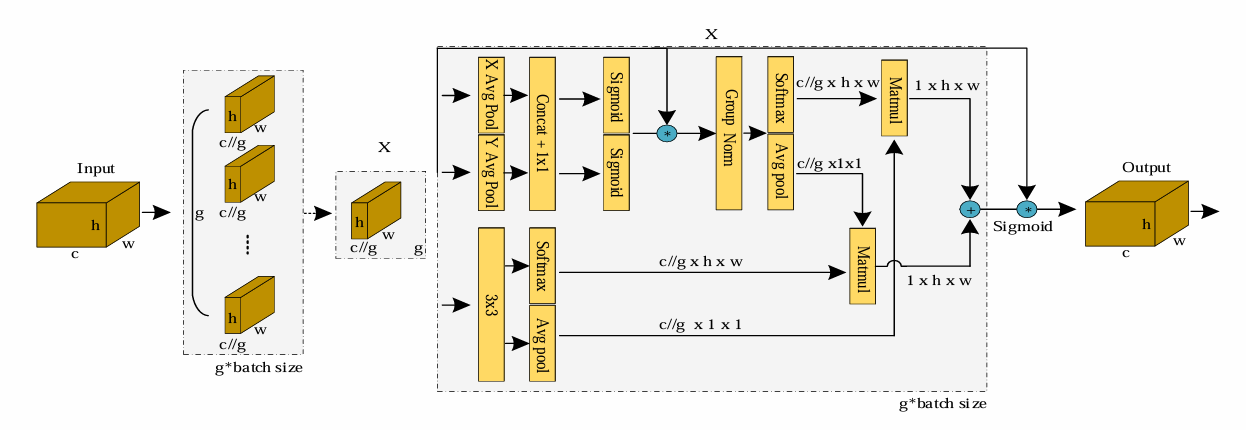
\includegraphics[width=0.85\textwidth]{Image/EMA_structure.png}
    \label{fig:ema_structure}
\end{figure}

Hình \ref{fig:ema_structure} thể hiện kiến trúc tổng quan của mô-đun EMA
(Efficient Multi-Scale Attention) \cite{ema2023}. Các mô-đun chú ý tiền nhiệm
như SE, CBAM hay CA đều sử dụng kỹ thuật giảm chiều kênh qua lớp kết nối đầy đủ
với tỉ lệ nén $r$, gây mất mát thông tin đặc trưng. EMA khắc phục hạn chế này
bằng cách xử lý theo nhóm kênh mà không giảm chiều.

Như thể hiện ở phần bên trái Hình \ref{fig:ema_structure}, bản đồ đặc trưng đầu
vào có kích thước $[C, H, W]$ --- trong đó $C$ là số kênh, $H$ là chiều cao,
$W$ là chiều rộng --- được chia thành $G$ nhóm, mỗi nhóm $C/G$ kênh.
Các nhóm được xử lý độc lập và song song; phần bên trong khung nét đứt mô tả luồng
tính toán cho một nhóm, gồm hai nhánh:

\textbf{Nhánh trên (Conv1$\times$1 + chú ý không gian):} Theo Hình
\ref{fig:ema_structure}, đầu vào $X$ đi qua hai khối gộp trung bình: X~Avg~Pool
gộp theo chiều $W$ tạo $pool\_h \in \mathbb{R}^{C/G \times H \times 1}$, và
Y~Avg~Pool gộp theo chiều $H$ tạo $pool\_w \in \mathbb{R}^{C/G \times 1 \times W}$.
Hai kết quả được ghép (Concat) thành tensor $[C/G,\; H+W,\; 1]$, đưa qua lớp tích
chập $1\times1$ rồi tách ra thành hai mặt nạ chú ý $x_h$ và $x_w$. Tiếp theo,
mỗi mặt nạ qua hàm Sigmoid rồi nhân phần tử ($\otimes$) với đầu vào $X$. Kết quả
được đưa qua khối Group~Norm để ổn định phân phối, cho ra $x_1$:
\begin{equation}
    x_1 = \text{GN}\!\left(\text{input} \cdot \sigma(x_h) \cdot \sigma(x_w)\right)
    \label{eq:ema_x1}
\end{equation}

\textbf{Nhánh dưới (Conv3$\times$3):} Như thể hiện ở nửa dưới Hình
\ref{fig:ema_structure}, đầu vào $X$ đi trực tiếp qua lớp tích chập $3\times3$ để
trích xuất đặc trưng cục bộ, cho ra $x_2$ có cùng kích thước $[C/G, H, W]$:
\begin{equation}
    x_2 = \text{Conv3}\times\text{3}(\text{input})
    \label{eq:ema_x2}
\end{equation}

\textbf{Kết hợp hai nhánh --- Học không gian chéo (Cross-spatial learning):}
Ở phần bên phải Hình \ref{fig:ema_structure}, mỗi nhánh được gộp trung bình toàn
cục (Avg~pool) xuống kích thước $[C/G, 1, 1]$, rồi áp Softmax để thu được vector
trọng số $[1, C/G]$. Vector này nhân ma trận (Matmul) với bản đồ đặc trưng đã
reshape $[C/G, H \times W]$ của nhánh còn lại, cho ra tensor $[1, H, W]$. Hai kết
quả matmul được cộng ($\oplus$):
\begin{equation}
    \text{weights} = \text{softmax}(\text{AGP}(x_1)) \cdot x_2^{\text{reshape}}
    + \text{softmax}(\text{AGP}(x_2)) \cdot x_1^{\text{reshape}}
    \;\in \mathbb{R}^{1 \times H \times W}
    \label{eq:ema_weights}
\end{equation}

Cuối cùng, tensor weights qua hàm Sigmoid rồi nhân phần tử ($\otimes$) với đầu vào
ban đầu để tạo đầu ra:
\begin{equation}
    \text{output} = \text{input} \cdot \sigma(\text{weights})
    \label{eq:ema_output}
\end{equation}
Hàm sigmoid đảm bảo trọng số nằm trong khoảng $(0, 1)$, đóng vai trò cổng chọn
lọc: vị trí có trọng số gần 1 được giữ nguyên, vị trí gần 0 bị triệt tiêu.

\section{Biểu diễn số thực dấu phẩy tĩnh (Fixed-Point Q8.8)}
Trong tính toán số trên phần cứng, có hai cách biểu diễn số thực phổ biến:
dấu phẩy động (IEEE 754) cho phạm vi rộng và độ chính xác cao nhưng đòi hỏi mạch
FPU phức tạp, tiêu tốn nhiều tài nguyên logic; dấu phẩy tĩnh biểu diễn số thực bằng
cách cố định vị trí dấu phẩy trong số nguyên nhị phân -- đơn giản hơn đáng kể,
phù hợp cho inference học sâu trên FPGA. Ký hiệu $Q_{m.n}$ mô tả định dạng với
$m$ bit phần nguyên (kể cả bit dấu) và $n$ bit phần lẻ, tổng $m+n$ bit. Giá trị
thực:
Định dạng Q8.8 được lựa chọn cho toàn bộ thiết kế: 16-bit có dấu, 8 bit phần
nguyên, 8 bit phần lẻ. Hệ số tỉ lệ là $2^8 = 256$, phạm vi biểu diễn
$[-128,\; 127{,}996]$ với độ phân giải $2^{-8} \approx 0{,}0039$.

Quy tắc tính toán trong Q8.8:
\begin{itemize}
    \item \textbf{Cộng/trừ:} Q8.8 $\pm$ Q8.8 $\to$ Q8.8, thực hiện trực tiếp trên
    số nguyên 16-bit.
    \item \textbf{Nhân:} Q8.8 $\times$ Q8.8 $\to$ Q16.16 (32-bit). Sau phép nhân
    phải dịch phải 8 bit để trở về Q8.8: $z = (a \times b) \gg 8$.
    \item \textbf{Tích lũy MAC:} Bộ tích lũy dùng 32-bit để tránh tràn số khi cộng
    nhiều tích Q8.8 liên tiếp (tối đa 144 lần trong Conv3$\times$3). Sau khi kết
    thúc vòng lặp, dịch phải 8 bit và cộng bias để ra kết quả Q8.8.
\end{itemize}

Toàn bộ tham số mô hình (weight, bias, $\gamma$, $\beta$ của GroupNorm) được lượng
tử hóa từ checkpoint PyTorch sang Q8.8 trước khi nạp vào BRAM ROM trên FPGA.

\section{Kiến trúc FSMD}
FSMD (Finite State Machine with Datapath) là kiến trúc mạch số kết hợp
hai thành phần tách biệt: một máy trạng thái hữu hạn (FSM) đóng vai trò Controller
điều phối trình tự hoạt động, và một Datapath thực hiện các phép tính số học theo
lệnh từ Controller.

\textbf{Controller (FSM)} nhận tín hiệu trạng thái từ Datapath (bộ đếm đã đến giá
trị cuối, phép chia hoàn thành, BRAM sẵn sàng) và sinh ra các tín hiệu điều khiển
(enable, load, clear, select) để điều phối Datapath. FSM được thiết kế theo mô hình
Moore (đầu ra chỉ phụ thuộc trạng thái hiện tại), đảm bảo hành vi đồng bộ và dễ
kiểm tra.

\textbf{Datapath} chứa toàn bộ logic tính toán: thanh ghi, bộ nhân, adder tree, bộ
đếm, MUX và kết nối tới BRAM. Datapath không có logic quyết định -- mọi điều kiện
rẽ nhánh đều do Controller xử lý.

Ưu điểm của FSMD: phân tách rõ ràng giữa logic điều khiển và logic tính toán giúp
dễ debug; mỗi khối con có Controller và Datapath riêng, cho phép phát triển và kiểm
tra độc lập trước khi tích hợp vào mô-đun top-level.

Trong thiết kế này, một số mô-đun sử dụng biến thể \textbf{pipeline thuần} thay vì
FSM đa trạng thái: các khối tính toán được nối thành chuỗi thanh ghi, nhận đầu vào
mới mỗi chu kỳ mà không cần chờ kết quả trước đó. FSM khi đó chỉ cần 3 giai đoạn
đơn giản: nạp pipeline, ghi kết quả, và xả pipeline. Kiến trúc
pipeline được áp dụng cho Sigmoid, Softmax, ElemMul, AddSigmoid và FinalMul.

\section{Bộ nhớ khối BRAM trên FPGA}
BRAM (Block RAM) là các khối bộ nhớ SRAM chuyên dụng tích hợp sẵn trên chip FPGA,
khác với Distributed RAM được tổng hợp từ LUT. Mỗi BRAM trên Artix-7 có dung lượng
36Kb, hỗ trợ chế độ đơn cổng (Simple Dual Port) và song cổng thực sự (True Dual
Port), với băng thông đọc/ghi độc lập trên mỗi cổng.

Trong thiết kế này, BRAM được sử dụng cho hai mục đích:
\begin{itemize}
    \item \textbf{ROM tham số:} Lưu weight và bias của Conv3$\times$3 (2304 giá trị),
    Conv1$\times$1 (256 giá trị), các hệ số $\gamma$, $\beta$ của GroupNorm, và các
    bảng LUT cho hàm exp. Các BRAM này được khởi tạo từ tệp .coe chứa tham số đã
    lượng tử hóa Q8.8, chỉ cần cổng đọc.
    \item \textbf{RAM bản đồ đặc trưng:} Lưu bản đồ đặc trưng trung gian giữa các khối tính
    toán. Dùng chế độ dual-port để cho phép đọc và ghi đồng thời ở hai cổng khác
    nhau. Nhiều BRAM được chia sẻ giữa các khối thông qua MUX điều khiển bởi FSM
    top-level.
\end{itemize}

Một đặc tính quan trọng: BRAM trên Artix-7 có độ trễ đọc (read latency) là
\textbf{2 chu kỳ clock} -- sau khi đặt địa chỉ lên cổng đọc, dữ liệu hợp lệ
xuất hiện ở đầu ra sau 2 chu kỳ. FSM trong mỗi Controller phải tính đến độ trễ
này và chèn trạng thái chờ phù hợp.

\chapter{THIẾT KẾ}
\section{Tổng quan kiến trúc thiết kế}

Mục này trình bày kiến trúc tổng thể của mô-đun EMA khi triển khai
trên phần cứng, bao gồm giao diện cổng top-level, datapath kết nối
các khối con, và máy trạng thái (FSM) điều phối toàn bộ pipeline.

\begin{figure}[h]{Mô-đun EMA tổng quan}
    \centering
    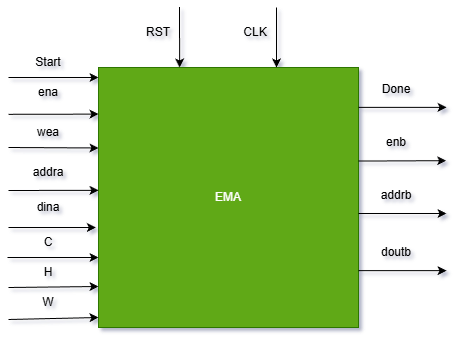
\includegraphics[width=0.7\textwidth]{Image/EMA_top_module.png}
    \label{fig:EMA_top_module_overview}
\end{figure}

Giao diện cổng của mô-đun top-level được thể hiện trong Hình \ref{fig:EMA_top_module_overview}. Mô-đun nhận hai nhóm tín hiệu đầu vào chính: nhóm điều khiển gồm \texttt{CLK}, \texttt{RST} và \texttt{Start} để đồng bộ và khởi động quá trình tính toán; nhóm giao diện BRAM cổng A gồm \texttt{ena}, \texttt{wea}, \texttt{addra} và \texttt{dina} để hệ thống bên ngoài nạp bản đồ đặc trưng đầu vào vào bộ nhớ nội bộ. Ngoài ra, ba tín hiệu \texttt{C}, \texttt{H}, \texttt{W} truyền kích thước tensor (số kênh, chiều cao, chiều rộng) vào mô-đun. Như đã trình bày ở Chương~1, phạm vi thiết kế giới hạn ở một nhóm trong $G = 32$ nhóm song song của khối đầu tiên thuộc giai đoạn 3 (ResNet50). Giai đoạn này có có 512 kênh, chia thành 32 nhóm, mỗi nhóm xử lý $C = 512/32 = 16$ kênh trên không gian $H = W = 16$; các tín hiệu \texttt{C}, \texttt{H}, \texttt{W} cho phép tham số hóa kích thước, nhưng trong thiết kế hiện tại được cố định: $C = 16$, $H = W = 16$.

Về phía đầu ra, tín hiệu \texttt{Done} báo hiệu mô-đun đã hoàn tất tính toán. Giao diện BRAM cổng B gồm \texttt{enb}, \texttt{addrb} và \texttt{doutb} cho phép hệ thống bên ngoài đọc bản đồ đặc trưng đầu ra sau khi \texttt{Done} được kéo lên mức cao. Việc tách riêng cổng ghi (Port A) và cổng đọc (Port B) theo giao thức BRAM dual-port giúp đơn giản hóa việc tích hợp mô-đun EMA vào pipeline xử lý lớn hơn mà không cần thêm logic đệm.

Toàn bộ giao tiếp nội bộ giữa các khối con - từ AvgPoolH/W, Conv1$\times$1, Conv3$\times$3, GroupNorm, Softmax đến Matmul và FinalMul - được thực hiện qua các BRAM nội bộ và tín hiệu handshake start/done cục bộ, tạo thành một pipeline kết hợp tuần tự và song song, có kiểm soát hoàn toàn bởi EMA\_controller.

\subsection{EMA Datapath}

Datapath gồm 12 khối tính toán và các BRAM trung gian kết nối theo
đúng luồng EMA (Hình~\ref{fig:EMA_datapath}). Dữ liệu đi qua hai
nhánh song song rồi hội tụ:

\begin{itemize}
    \item \textbf{Nhánh 1 (chú ý không gian)}:
    Input $\to$ AvgPoolH $\to$ AvgPoolW $\to$ ghép nối (cat) vào
    BRAM 512 $\to$ Conv1x1 $\to$ Sigmoid $\xrightarrow{\text{Split}}$
    sig\_h + sig\_w $\to$ ElemMul (với input gốc) $\to$ GroupNorm
    $\to$ x1

    \item \textbf{Nhánh 2 (conv3x3)}: Input $\to$ Conv3x3 $\to$ x2.
    Conv3x3 chạy \textbf{song song} với nhánh 1 — FSM giữ
    \texttt{Start\_Conv33 = '1'} suốt từ \texttt{S\_AvgH} đến
    \texttt{S\_GroupNorm}. Trạng thái \texttt{S\_GroupNorm} chờ cả
    \texttt{Done\_GroupNorm} và \texttt{Done\_Conv33} mới chuyển tiếp.

    \item \textbf{Cross-spatial learning}: x1 và x2 đi vào hai nhánh
    đối xứng:
    \begin{itemize}
        \item AvgPool(x1) $\to$ Softmax $\to$ Matmul(softmax,
        \textbf{x2}) $\to$ x12
        \item AvgPool(x2) $\to$ Softmax $\to$ Matmul(softmax,
        \textbf{x1}) $\to$ x21
    \end{itemize}
    Hai nhánh AvgPool, Softmax, Matmul chạy \textbf{song song}
    (cùng nhận Start, Done hội tụ bằng AND).

    \item \textbf{Kết hợp}: AddSigmoid cộng hai kết quả Matmul rồi
    áp sigmoid $\to$ weights. FinalMul nhân input gốc với weights $\to$
    output.
\end{itemize}

\begin{figure}[p]{Datapath tổng quan của mô-đun EMA}
    \centering
    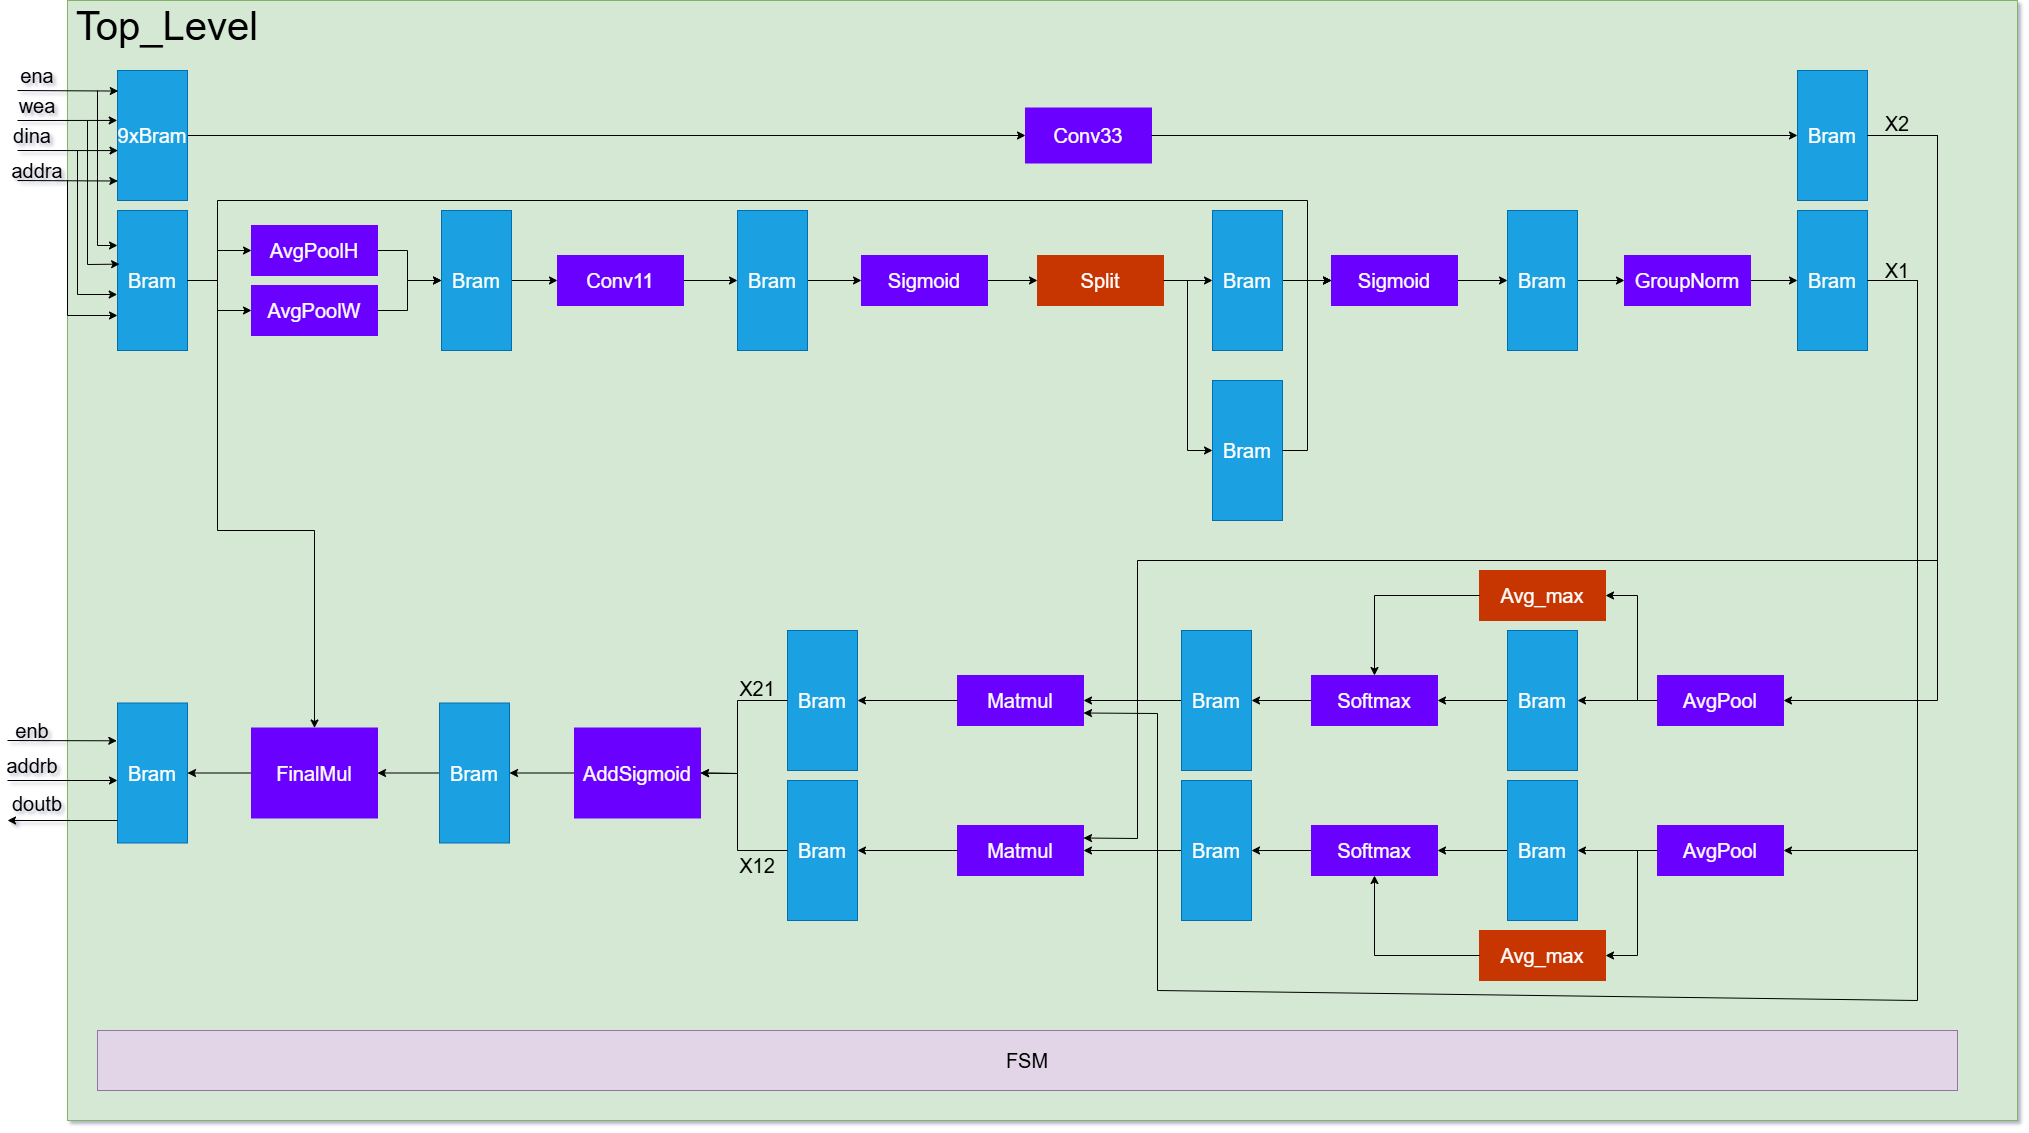
\includegraphics[width=0.95\textheight, angle=270]{Image/EMA_datapath.png}
    \label{fig:EMA_datapath}
\end{figure}

\newpage

Ngoài các khối tính toán chính, datapath còn có hai khối phụ trợ:

\begin{enumerate}
    \item \textbf{Split}
\end{enumerate}
\begin{figure}[h]{Khối Split}
    \centering
    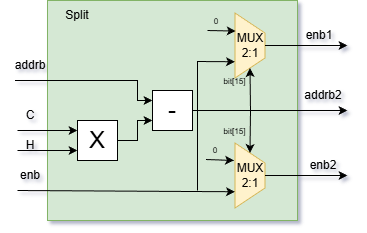
\includegraphics[width=0.45\textwidth]{Image/Split.png}
    \label{fig:Split}
\end{figure}
\begin{itemize}
    \item Đầu ra Sigmoid có kích thước $[C, H{+}W]$ (do Conv1x1 nhận
    đầu vào ghép nối pool\_h và pool\_w). Khối Split tách thành
    sig\_h $[C, H]$ và sig\_w $[C, W]$ bằng cách so sánh địa chỉ ghi
    \texttt{addra} với ngưỡng $CH$: nếu $\texttt{addra} < CH$
    thì ghi vào BRAM sig\_h (\texttt{enb1 = '1'}), ngược lại ghi vào
    BRAM sig\_w (\texttt{enb2 = '1'}) với địa chỉ đã trừ $CH$.
    Split hoàn toàn tổ hợp, không thêm trễ pipeline.
\end{itemize}

\begin{enumerate}
    \setcounter{enumi}{1}
    \item \textbf{Avg\_max}
\end{enumerate}
\begin{figure}[h]{Khối Avg\_max}
    \centering
    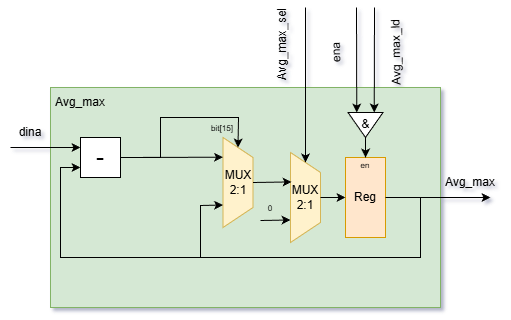
\includegraphics[width=0.5\textwidth]{Image/AvgMax.png}
    \label{fig:AvgMax}
\end{figure}
\begin{itemize}
    \item Softmax cần giá trị $x_{\max}$ để dịch đầu vào trước khi
    tính exp. Khối Avg\_max tìm giá trị lớn nhất trong đầu ra AvgPool
    \textbf{ngay trong lúc AvgPool đang ghi}: mỗi khi AvgPool ghi một
    giá trị \texttt{dina}, khối so sánh $\texttt{dina} - \texttt{Avg\_max}$
    — nếu kết quả dương (bit dấu = '0') thì cập nhật \texttt{Avg\_max}
    bằng \texttt{dina}, ngược lại giữ nguyên. MUX thứ hai reset
    \texttt{Avg\_max} về 0 khi \texttt{Avg\_max\_sel = '0'} (trước mỗi
    lượt AvgPool mới). Mỗi nhánh AvgPool có một instance Avg\_max
    riêng.
\end{itemize}

\textbf{Quản lý BRAM trung gian}: tổng cộng datapath sử dụng
10 BRAM đầu vào (9$\times$Bram4096 cho Conv3x3 và 1$\times$Bram4096 cho các khối còn lại) cùng 8 BRAM trung gian các kích thước (Bram512, Bram256,
Bram16, Bram4096). BRAM input được chia sẻ giữa
AvgPoolH, AvgPoolW, ElemMul và FinalMul thông qua MUX điều khiển bởi
tín hiệu từ FSM. Tương tự, BRAM
GroupNorm và BRAM Conv3x3 cũng được chia sẻ giữa AvgPool/Matmul.

\subsection{EMA Controller}

\begin{figure}[h]{FSM điều khiển mô-đun EMA}
    \centering
    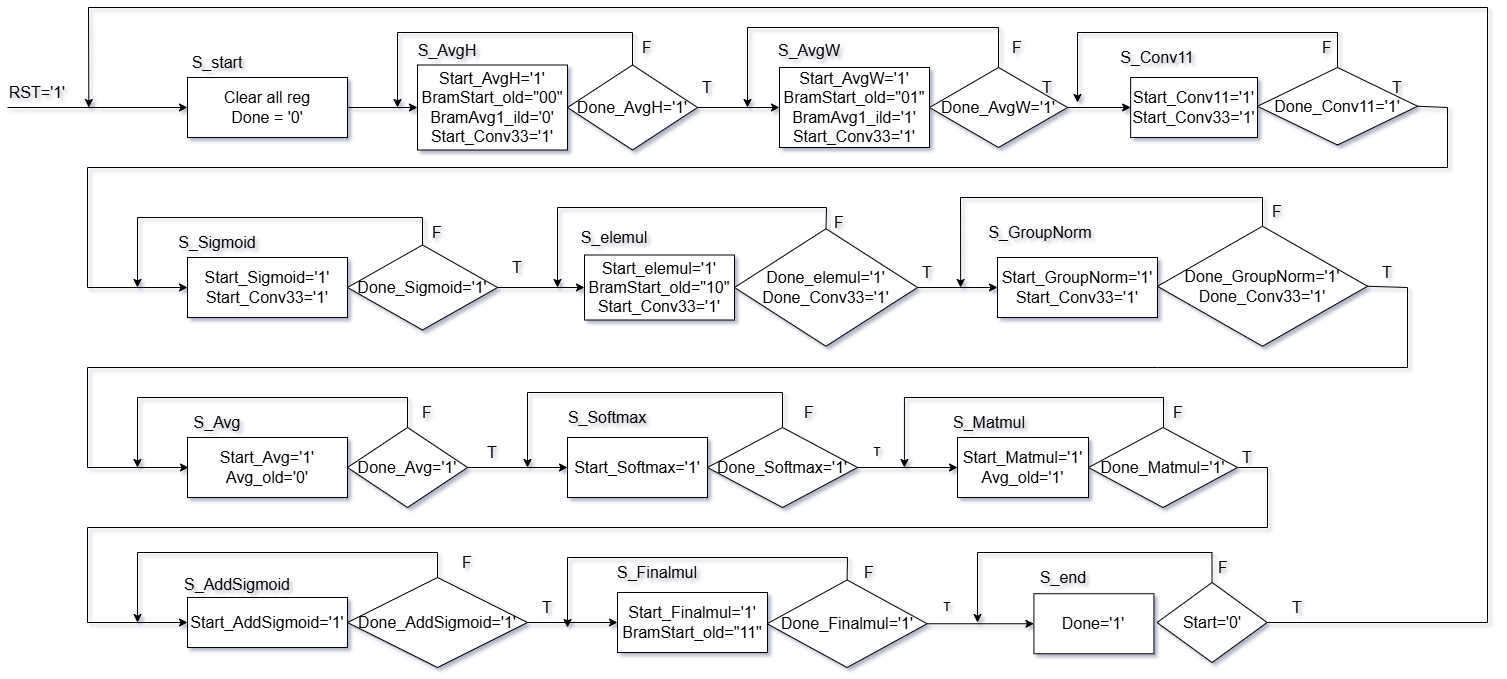
\includegraphics[width=0.75\textheight, angle = 270]{Image/EMA_controller.png}
    \label{fig:EMA_FSM}
\end{figure}
\begin{itemize}
    \item FSM gồm 14 trạng thái, mỗi trạng thái tương ứng kích hoạt
    một (hoặc nhiều) khối con:

    \item \texttt{S\_start}: chờ \texttt{Start\_i = '1'}.

    \item \texttt{S\_AvgH}: kích hoạt AvgPoolH và Conv3x3 (song song).
    \texttt{BramStart\_old = "00"} — BRAM input nối với AvgPoolH. Chờ
    \texttt{Done\_AvgH}.

    \item \texttt{S\_AvgW}: kích hoạt AvgPoolW (Conv3x3 vẫn chạy).
    \texttt{BramStart\_old = "01"} — BRAM input nối với AvgPoolW.
    \texttt{BramAvg1\_ild = '1'} — chuyển BRAM ghép nối sang ghi
    pool\_w (nối tiếp sau pool\_h). Chờ \texttt{Done\_AvgW}.

    \item \texttt{S\_Conv11}: kích hoạt Conv1x1. Chờ
    \texttt{Done\_Conv11}.

    \item \texttt{S\_Sigmoid}: kích hoạt Sigmoid (kết quả tự tách qua
    Split). Chờ \texttt{Done\_Sigmoid}.

    \item \texttt{S\_elemul}: kích hoạt ElemMul.
    \texttt{BramStart\_old = "10"} — BRAM input nối với ElemMul (đọc
    input gốc). Chờ \texttt{Done\_elemul}.

    \item \texttt{S\_GroupNorm}: kích hoạt GroupNorm (Conv3x3 vẫn chạy).
    \texttt{Avg\_max\_ld = '1'} — reset Avg\_max về 0 chuẩn bị cho
    AvgPool. Chờ \textbf{cả} \texttt{Done\_GroupNorm} và
    \texttt{Done\_Conv33}.

    \item \texttt{S\_Avg}: kích hoạt 2 instance AvgPool song song (một
    cho x1/GroupNorm, một cho x2/Conv3x3).
    \texttt{Avg\_max\_sel = '1'} — bật cập nhật Avg\_max. Chờ
    \texttt{Done\_Avg = Done\_Avg1 AND Done\_Avg2}.

    \item \texttt{S\_Softmax}: kích hoạt 2 instance Softmax song song,
    mỗi instance nhận \texttt{Avg\_max} tương ứng. Chờ
    \texttt{Done\_Softmax = Done\_Softmax1 AND Done\_Softmax2}.

    \item \texttt{S\_Matmul}: kích hoạt 2 instance Matmul song song
    (cross: softmax1$\times$x2, softmax2$\times$x1).
    \texttt{Avg\_old = '1'} — chuyển MUX BRAM GroupNorm/Conv3x3 sang
    phục vụ Matmul. Chờ
    \texttt{Done\_Matmul = Done\_Matmul1 AND Done\_Matmul2}.

    \item \texttt{S\_AddSigmoid}: kích hoạt AddSigmoid. Chờ
    \texttt{Done\_AddSigmoid}.

    \item \texttt{S\_Finalmul}: kích hoạt FinalMul.
    \texttt{BramStart\_old = "11"} — BRAM input nối với FinalMul (đọc
    input gốc lần cuối). Chờ \texttt{Done\_Finalmul}.

    \item \texttt{S\_end}: bật \texttt{Done\_o = '1'}, chờ
    \texttt{Start\_i} hạ.
\end{itemize}

Điểm đáng chú ý của FSM top-level là sự kết hợp \textbf{tuần tự và
song song}: Conv3x3 chạy song song với toàn bộ nhánh 1 (tiết kiệm
đáng kể thời gian), hai nhánh AvgPool/Softmax/Matmul chạy song song
với nhau, trong khi các bước còn lại chạy tuần tự. Tín hiệu
\texttt{BramStart\_old} và \texttt{Avg\_old} đóng vai trò bộ chuyển
mạch, cho phép nhiều khối chia sẻ cùng BRAM mà không xung đột nhờ
không bao giờ truy cập đồng thời.

\section{Các khối tính toán cơ bản}
\subsection{Bộ nhân}
Bộ nhân trong dự án được thiết kế bằng kiến trúc Booth-Wallace, nhận vào 2 số đầu vào \texttt{a}, \texttt{b} và xuất kết quả \texttt{result}.
\begin{figure}[h]{Bộ nhân}
    \centering
    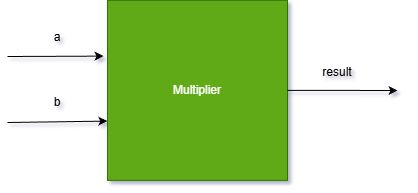
\includegraphics[width=0.7\textwidth]{Image/bonhantop.png}
    \label{Mul_top}
\end{figure}

\textbf{Phương pháp tính:}
Phép nhân hai số nhị phân $m$-bit được thực hiện bằng cách tạo $m$
tích thành phần, mỗi tích thành phần là số bị nhân $a$ dịch trái
theo vị trí bit tương ứng của số nhân $b$. Kết quả cuối cùng là tổng
của tất cả tích riêng phần, cho ra tích $2m$-bit. Tuy nhiên, cộng
trực tiếp $m$ số nhiều bit gây trễ lan truyền nhớ lớn và tốn nhiều
tài nguyên. Hai kỹ thuật được áp dụng để giải quyết vấn đề này: mã
hóa Booth Radix-4 giảm số tích riêng phần đi một nửa, và cây Wallace
nén nhiều số thành hai số bằng bộ cộng không lan truyền nhớ
\cite{booth_wallace}.

\begin{table}[h]{Bảng mã hóa Booth Radix-4}
        \centering
        \begin{tabular}{ccc|c}
            $b_{i+1}$ & $b_i$ & $b_{i-1}$ & Partial product \\ \hline
            0 & 0 & 0 & $0$   \\
            0 & 0 & 1 & $+a$  \\
            0 & 1 & 0 & $+a$  \\
            0 & 1 & 1 & $+2a$ \\
            1 & 0 & 0 & $-2a$ \\
            1 & 0 & 1 & $-a$  \\
            1 & 1 & 0 & $-a$  \\
            1 & 1 & 1 & $0$   \\
        \end{tabular}
        \label{tab:booth}
    \end{table}
\begin{itemize}
    \item \textbf{Modified Booth Encoding (Radix-4)}: Số nhân $b$ ($m$-bit) được
    mở rộng thành $(m+2)$-bit rồi chia thành
    $m/2$ nhóm 3-bit $(b_{2i+2},\, b_{2i+1},\, b_{2i})$ với
    $i = 0..\frac{m}{2}-1$. Mỗi nhóm được đưa vào một \texttt{booth\_encoder}
    để sinh ra tích thành phần $(m+2)$-bit theo Bảng \ref{tab:booth}. Từ đó,
    với đầu vào $m$-bit, ta chỉ cần $m/2$ tích thành phần thay vì $m$ như
    phương pháp thông thường. Sau khi sinh xong, mỗi tích thành phần được
    mở rộng dấu lên $2m$-bit và dịch trái theo vị trí bit tương ứng
    ($pp_i \ll 2i$) trước khi đưa vào tầng Wallace Tree.
\end{itemize}
\begin{figure}[h]{Kiến trúc Wallace Tree 4 tầng CSA}
    \centering
    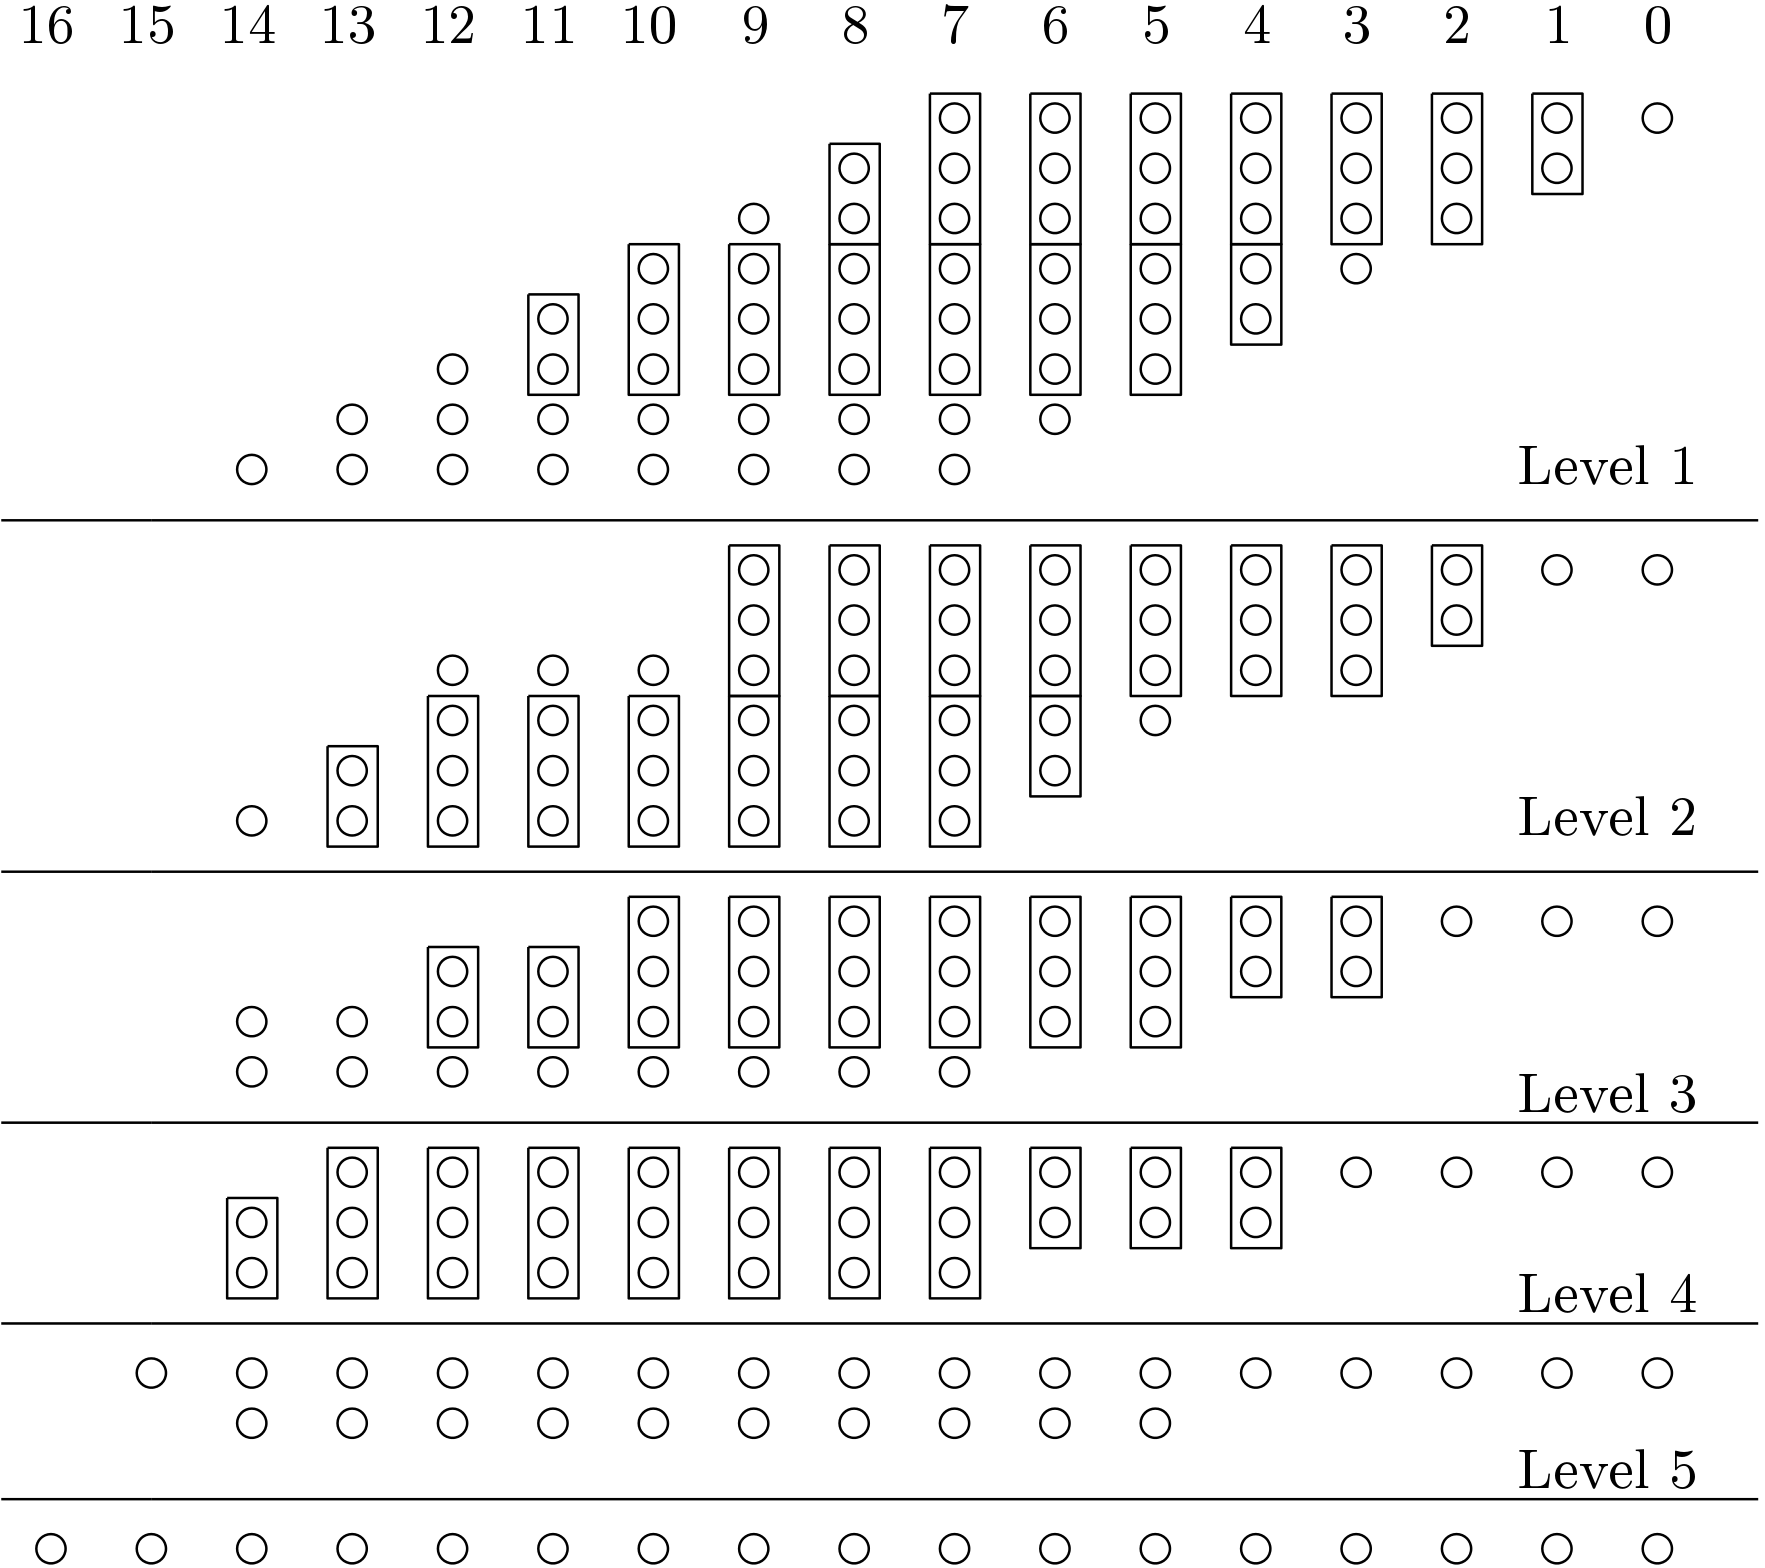
\includegraphics[width=0.7\textwidth]{Image/wallace_tree.png}
    \label{fig:wallace}
\end{figure}
\begin{itemize}
    \item  \textbf{Wallace Tree}: Nhận $m/2$ tích thành phần từ tầng
    Booth và nén xuống còn 2 số (\texttt{wsum}, \texttt{wcarry}) qua
    nhiều tầng Carry-Save Adder (CSA) song song. Mỗi CSA nhận 3 đầu
    vào $A$, $B$, $C$ và tính:
    \begin{equation}
    \begin{aligned}
        \text{sum}   &= A \oplus B \oplus C \\
        \text{carry} &= \left[(A \wedge B) \vee (B \wedge C)
                        \vee (A \wedge C)\right] \ll 1
    \end{aligned}
    \end{equation}

    Quá trình nén được minh họa bằng biểu đồ chấm (dot diagram) ở
    Hình~\ref{fig:wallace}. Mỗi cột ứng với một vị trí bit (đánh số
    0--16 từ phải sang trái), mỗi chấm tròn biểu diễn một bit tại cột
    đó. Khi 3 chấm trong cùng một cột được nhóm trong hình chữ nhật,
    chúng được đưa vào một Full Adder (3:2), sinh ra 1 bit tổng giữ
    nguyên cột và 1 bit nhớ chuyển sang cột bên trái. Các chấm không
    đủ bộ 3 truyền thẳng xuống tầng tiếp theo.

    Với $m/2 = 8$ tích thành phần, cây Wallace nén qua 4 tầng: tầng 1
    dùng 2 CSA song song nén 8 số xuống 4; tầng 2 nén xuống 3; tầng 3
    và 4 lần lượt nén xuống 2 số cuối cùng là \texttt{wsum} và
    \texttt{wcarry}. Toàn bộ các tầng hoạt động tổ hợp song song,
    không có thanh ghi trung gian, cho phép hoàn thành phép nhân trong
    một chu kỳ clock.

    Hai số \texttt{wsum} và \texttt{wcarry} được cộng lại bằng bộ cộng
    của thư viện IEEE.NUMERIC\_STD để ra tích $2m$-bit cuối cùng. Tùy
    theo định dạng $Q_{m.n}$ đang sử dụng mà lấy các bit tương ứng
    của kết quả làm đầu ra \texttt{result}.
\end{itemize}

Sau khi tính toán đầu ra, ta xử lý bão hòa bằng cách kiểm tra các bit cao, nếu tất cả đồng nhất (toàn 0 hoặc toàn 1) thì không tràn
số, ngược lại, nếu không đồng nhất thì đã tràn số và kết quả được làm tròn về tràn dương hoặc tràn âm

Trong đồ án, bộ nhân được thiết kế để hỗ trợ cả hai định dạng 16-bit và 32-bit. Đặc biệt, đối với phép nhân 32-bit, một tầng thanh ghi (register) được bổ sung vào luồng dữ liệu nhằm rút ngắn đường trễ tới hạn (critical path), đảm bảo mạch hoạt động ổn định ở tần số 100 MHz
\subsection{Bộ chia}
Bộ chia được thiết kế theo thuật toán Goldschmidt --- phương pháp chia
lặp dựa trên phép nhân \cite{goldschmidt1964}. Gọi $X$ là tử số,
$Y$ là mẫu số cần tính $X/Y$. Thuật toán nhân đồng thời cả $X_k$ và
$Y_k$ với hệ số hiệu chỉnh $F_k = 2 - Y_k$ qua mỗi vòng lặp:
\begin{equation}
    X_{k+1} = X_k \cdot F_k, \quad
    Y_{k+1} = Y_k \cdot F_k, \quad
    F_k = 2 - Y_k
\end{equation}
Do $0.5 \leq Y_0 < 1$ (sau chuẩn hóa), mỗi vòng lặp đưa $Y_k$ tiến
gần 1 hơn, khi đó $X_k$ hội tụ về thương $X/Y$.

Bộ chia được thiết kế theo kiến trúc FSMD:
\begin{enumerate}
    \item \textbf{Datapath}
\end{enumerate}
\begin{itemize}
    \item Bộ chia nhận 2 số đầu vào $X$, $Y$ với điều kiện $Y > 0$. Bit dấu
    của $X$ được kiểm tra để xác định dấu kết quả - nếu $X < 0$, datapath
    lấy $X \leftarrow -X$ trước khi tính và đảo dấu kết quả ở đầu ra.

    \item Tiếp theo, $X$ và $Y$ được chuẩn hóa về khoảng $[0.5,\; 1)$ bằng
    barrel shifter. Thiết kế kiểm tra byte cao của $Y$ để xác định hướng dịch:
    nếu $Y \geq 1$ (byte cao khác 0) thì dịch phải $X$, $Y$ một lượng $s_R$
    tra từ LUT theo các bit cao; nếu $Y < 1$ (byte cao bằng 0) thì dịch trái
    một lượng $s_L$ tra từ LUT theo các bit thấp:
    \begin{equation}
        (X_{norm},\; Y_{norm}) =
        \begin{cases}
            (X \gg s_R,\; Y \gg s_R) & \text{nếu } Y \geq 1 \\
            (X \ll s_L,\; Y \ll s_L) & \text{nếu } Y < 1
        \end{cases}
        \quad \text{sao cho } 0.5 \leq Y_{norm} < 1
    \end{equation}

    \item Cuối cùng, thuật toán Goldschmidt được lặp $k$ lần. Sau $k$ vòng lặp, $Y_k \to 1$ và $X_k \to X/Y$. Với định dạng 16-bit,
    $k = 3$ là đủ để đảm bảo sai số nhỏ hơn $2^{-7}$.
\end{itemize}

\newpage

\begin{figure}[h]{Datapath bộ chia}
    \centering
    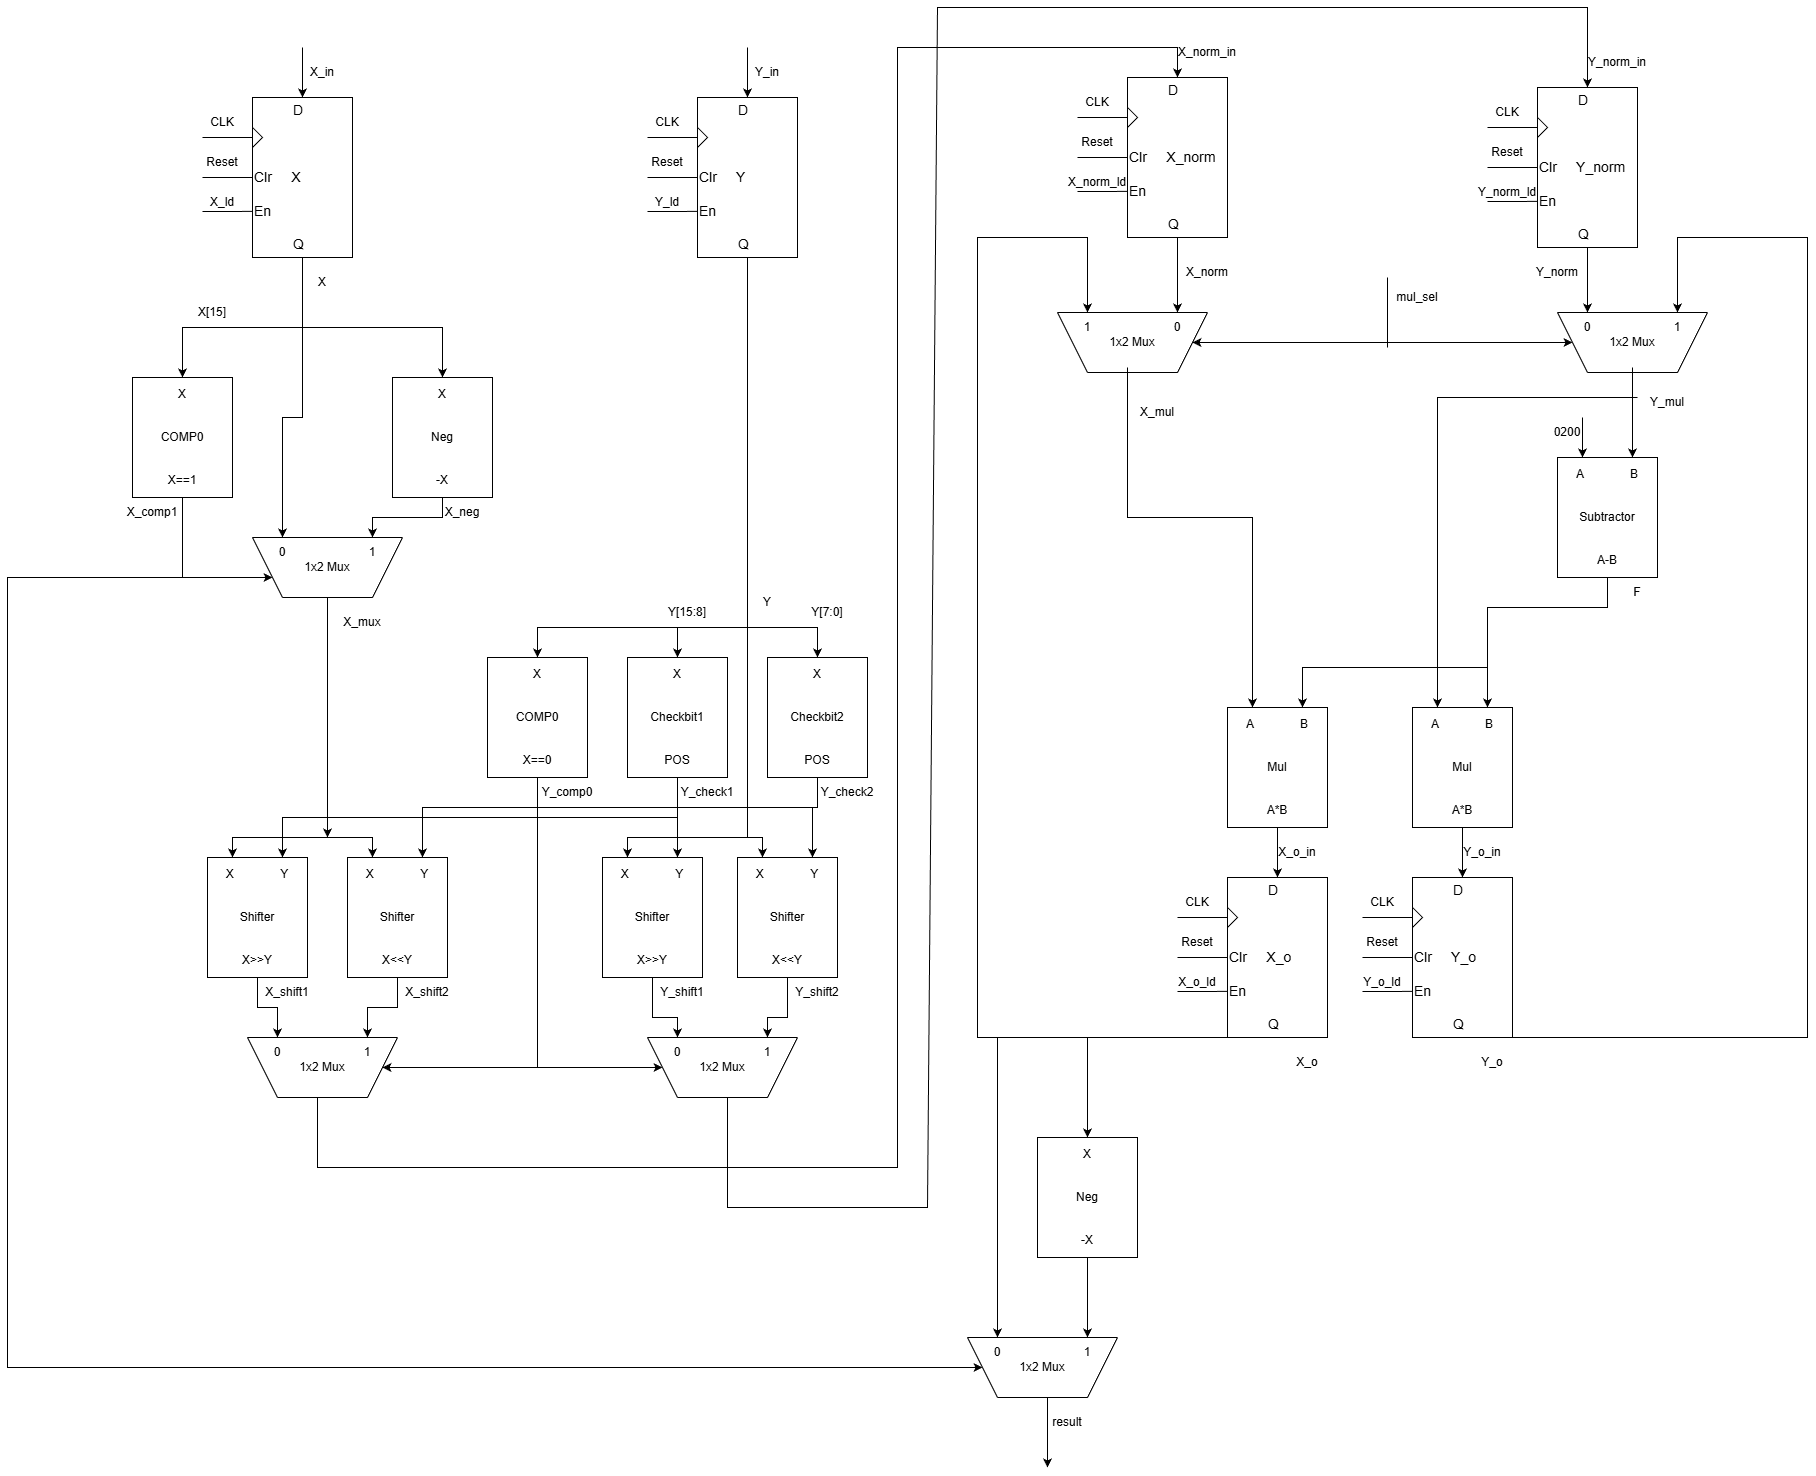
\includegraphics[width=0.7\textheight, angle = 270]{Image/Div_datapath.png}
    \label{fig:Div_datapath}
\end{figure}

\begin{enumerate}
    \setcounter{enumi}{1}
    \item \textbf{FSM}
\end{enumerate}

\begin{itemize}
    \item FSM gồm 11 trạng thái (S0 -- S10). S1 chờ \texttt{Start\_i}.
    S2 nạp đầu vào, S3 chuẩn hóa $X$, $Y$ về khoảng $[0.5,\;1)$.

    \item Ba cặp trạng thái S4--S5, S6--S7, S8--S9 thực hiện ba vòng lặp
    Goldschmidt: trạng thái lẻ tính $F_k = 2 - Y_k$, trạng thái chẵn
    cập nhật $X_{k+1} = X_k \cdot F_k$, $Y_{k+1} = Y_k \cdot F_k$.

    \item S9 bật \texttt{Done\_o}. S10 giữ kết quả đến khi \texttt{Start\_i}
    hạ xuống '0'.
\end{itemize}

\newpage

\begin{figure}[h]{FSM bộ chia}
    \centering
    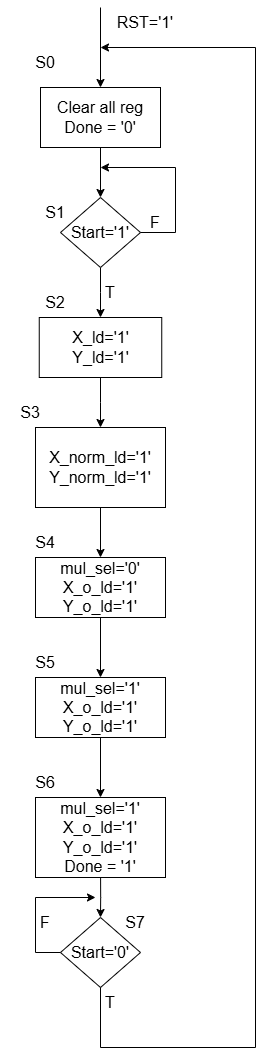
\includegraphics[width=0.25\textwidth]{Image/Division_FSM.png}
    \label{fig:Div_FSM}
\end{figure}

Để áp dụng kiến trúc đường ống (pipeline) cho bộ chia nhằm tăng thông lượng, thiết kế tiến hành ghép nối tuần tự nhiều khối Goldschmidt. Đồng thời, khi xử lý toán hạng 32-bit, hệ thống máy trạng thái (FSM) tự động tính toán độ trễ chu kỳ của bộ nhân để chèn các trạng thái chờ một cách đồng bộ
\subsection{Bộ căn bậc hai}
Bộ căn bậc 2 tính theo thuật toán Newton-Raphson \cite{korzilius2023}. Xuất phát từ một giá trị khởi tạo $x_0$, thuật toán lặp
\begin{equation}
    x_{k+1} = \frac{x_k + \dfrac{S}{x_k}}{2}
\end{equation}
trong đó $S$ là số cần tính căn. Sau $k$ vòng lặp, $x_k$ hội tụ về
$\sqrt{S}$. Với định dạng Q8.8 (16-bit), 4 vòng lặp là đủ để đảm bảo sai
số nhỏ hơn $2^{-7}$.

Bộ căn bậc hai được thiết kế theo phương pháp FSMD:

\begin{enumerate}
    \item \textbf{Datapath}
\end{enumerate}
\begin{figure}[h]{Datapath bộ căn bậc hai}
    \centering
    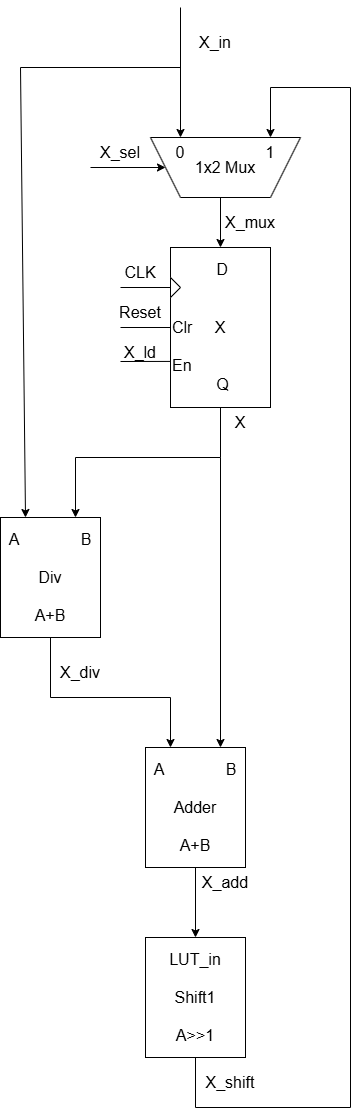
\includegraphics[width=0.35\textwidth]{Image/SQRT_datapath.png}
    \label{fig:SQRT_datapath}
\end{figure}
\begin{itemize}
    \item Giá trị khởi tạo $x_0 = S$ (chính là đầu vào \texttt{X\_in}).
    Một MUX chọn giữa $x_0$ (vòng đầu) và kết quả vòng lặp trước đó.

    \item Mỗi vòng lặp thực hiện 3 bước tuần tự:
    \begin{itemize}
        \item[$-$] Chia: gọi bộ \texttt{Div\_16bit} tính $X_{div} = S / x_k$
        \item[$-$] Cộng: $X_{add} = x_k + X_{div}$
        \item[$-$] Dịch phải 1 bit: $x_{k+1} = X_{add} \gg 1$ (tương đương chia 2)
    \end{itemize}

    \item Kết quả $x_{k+1}$ được nạp lại vào thanh ghi \texttt{X} qua MUX
    để chuẩn bị cho vòng lặp tiếp theo. Sau 4 vòng, giá trị trong thanh ghi
    chính là $\sqrt{S}$ ở định dạng Q8.8.
\end{itemize}
\begin{enumerate}
    \setcounter{enumi}{1}
    \item \textbf{FSM}
\end{enumerate}
\begin{figure}[h]{FSM bộ căn bậc hai}
    \centering
    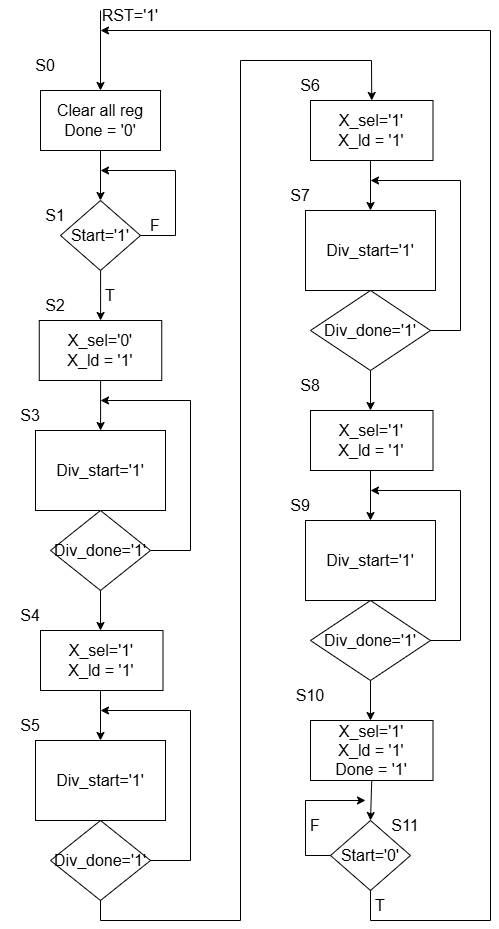
\includegraphics[width=0.5\textwidth]{Image/SQRT_FSM.png}
    \label{fig:SQRT_FSM}
\end{figure}
\begin{itemize}
    \item FSM gồm 12 trạng thái (S0 -- S11). S1 chờ tín hiệu
    \texttt{Start\_i}. Mỗi vòng lặp Newton-Raphson chiếm 2 trạng thái:
    một trạng thái nạp giá trị mới vào thanh ghi (S2, S4, S6, S8) và một
    trạng thái kích hoạt bộ chia rồi chờ \texttt{Div\_done} (S3, S5, S7, S9).

    \item S10 nạp kết quả vòng lặp cuối và bật \texttt{Done\_o}. S11 giữ
    kết quả cho đến khi \texttt{Start\_i} được hạ xuống '0'.
\end{itemize}
\subsection{Bộ e mũ}

Bộ tính $e^x$ được thiết kế theo phương pháp tra bảng LUT kết hợp
nhân pipeline, xử lý cả đầu vào dương lẫn âm theo định dạng Q8.8.

Ý tưởng phân tách:
\begin{equation}
    e^x = C \times e^{x_{int}} \times e^{x_{frac\_high}}
          \times e^{x_{frac\_low}}
\end{equation}
trong đó $x_{int}$ lấy từ bit [11:8], $x_{frac\_high}$ từ bit [7:4]
và $x_{frac\_low}$ từ bit [3:0] của $|x|$. Hệ số $C = 1{,}0$ khi
$|x| \leq 15$ (dải LUT hợp lệ), bằng $0$ khi vượt dải để tránh tràn số.

\begin{figure}[h]{Datapath bộ e mũ}
    \centering
    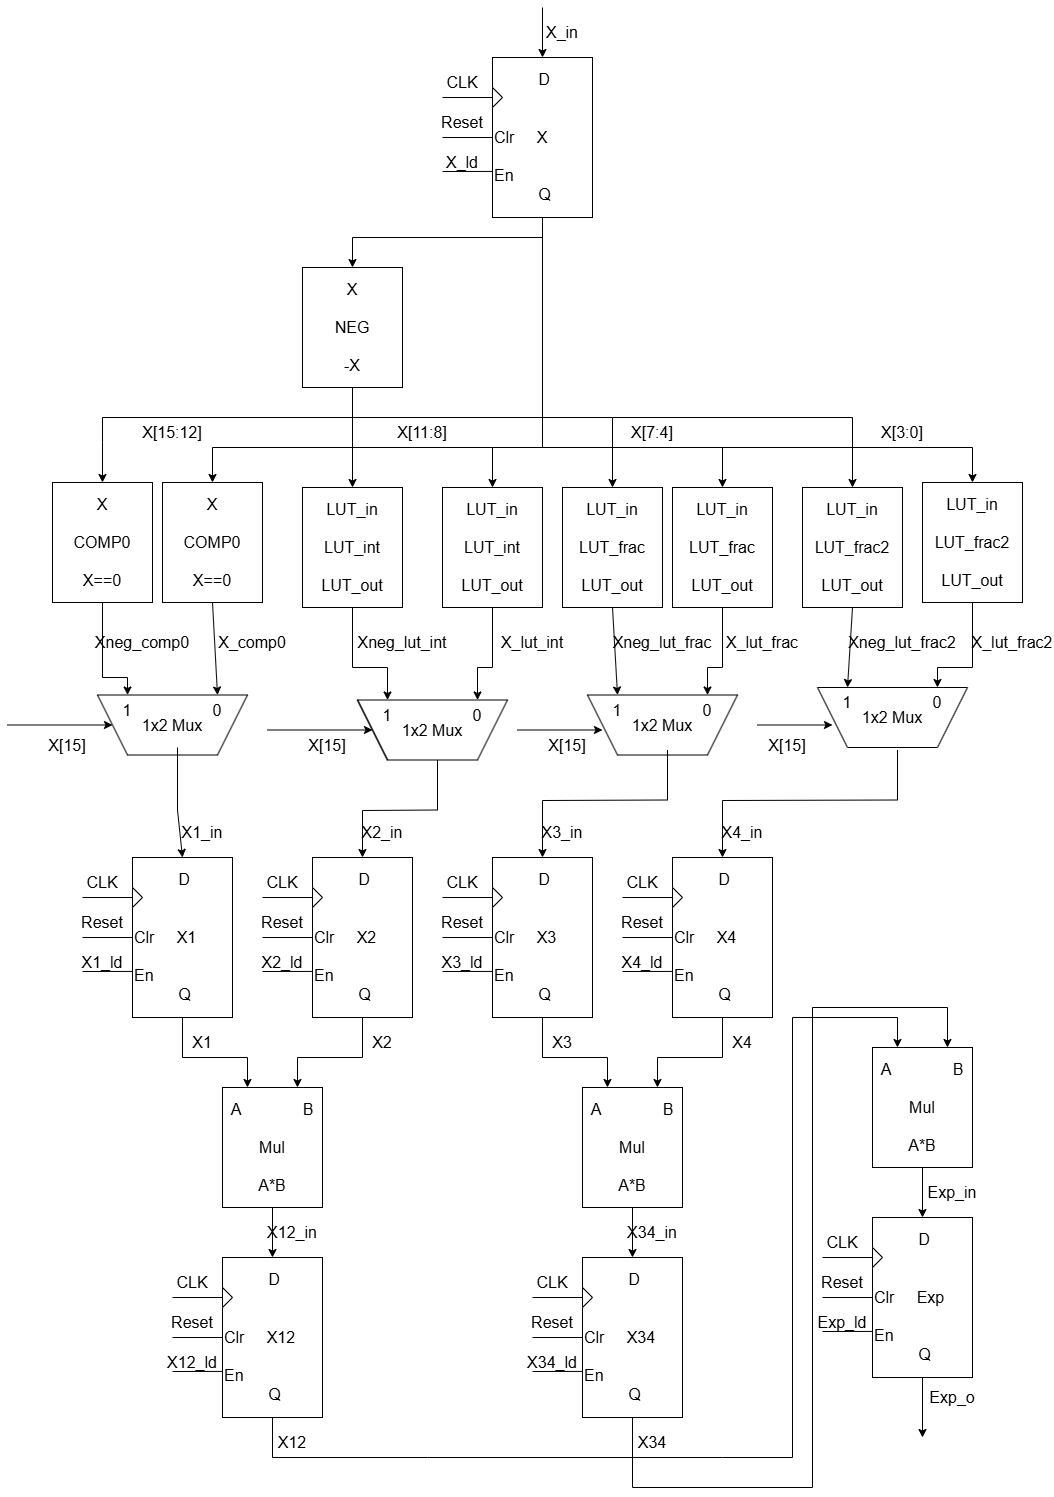
\includegraphics[width=0.75\textwidth]{Image/Exp_datapath.png}
    \label{fig:Exp_datapath}
\end{figure}

Bộ này được thiết kế để pipeline nên không có FSM mà chỉ có datapath, latency cố định \textbf{4 chu kỳ clock}:

\begin{itemize}
    \item \textbf{Chu kỳ 1}: Nạp \texttt{X\_in} → thanh ghi $X$,
    tính $-X$ nếu $x<0$ vì số dương nhị phân dễ xử lý hơn.

    \item \textbf{Chu kỳ 2}: Tra song song hai bộ LUT kép —
    \texttt{exp\_lut\_*} (địa chỉ từ $X$) và \texttt{expneg\_lut\_*}
    (địa chỉ từ $-X$). Bốn MUX 2-1 chọn kết quả theo bit dấu
    \texttt{X[15]}: nếu $x \geq 0$ dùng LUT dương, ngược lại dùng
    LUT âm. Nạp $X_1$, $X_2$, $X_3$, $X_4$.

    \item \textbf{Chu kỳ 3}: Hai bộ nhân Booth-Wallace chạy song song:
    $X_{12} = X_1 \times X_2$, $\; X_{34} = X_3 \times X_4$.

    \item \textbf{Chu kỳ 4}: $e^x = X_{12} \times X_{34}$, kết quả
    ra \texttt{Exp\_o}.
\end{itemize}
\subsection{Bộ lặp}
Bộ lặp là thành phần dùng chung trong nhiều mô-đun (Conv3x3, AvgPoolH,
AvgPoolW, ...) để tạo ra các chỉ số vòng lặp đa chiều. Mỗi chiều gồm
một bộ đếm độc lập có cấu trúc giống nhau như Hình \ref{fig:Counter}.

\begin{figure}[h]{Cấu trúc bộ lặp}
    \centering
    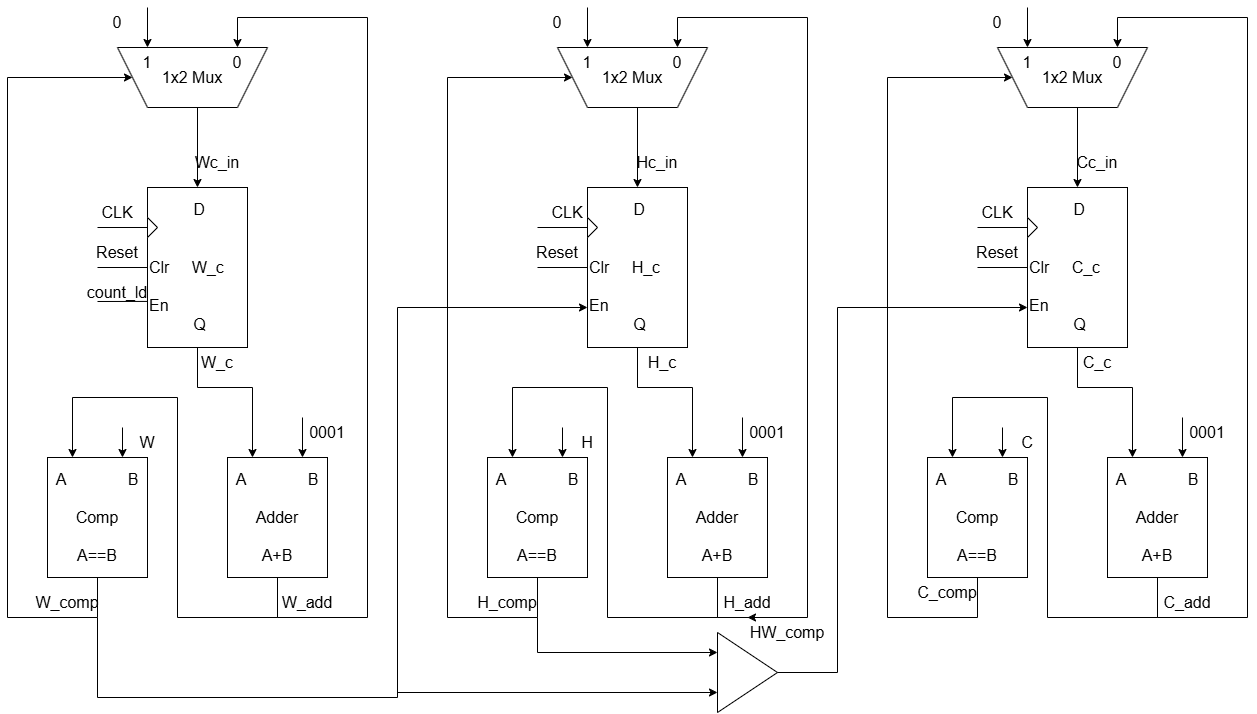
\includegraphics[width=\textwidth]{Image/Counter.png}
    \label{fig:Counter}
\end{figure}

Mỗi bộ đếm gồm ba khối:
\begin{itemize}
    \item \textbf{Adder}: tính $count + 1$ ở mỗi chu kỳ.
    \item \textbf{Comp}: so sánh giá trị hiện tại với ngưỡng
    tối đa (W, H hoặc C). Khi bằng nhau, tín hiệu \texttt{comp = '1'}.
    \item \textbf{MUX + Register}: MUX chọn giữa $0$ (khi
    \texttt{comp = '1'}, reset về đầu) và $count + 1$ (khi chưa đạt
    ngưỡng). Kết quả được nạp vào thanh ghi qua tín hiệu
    \texttt{count\_ld}.
\end{itemize}

Các bộ đếm được ghép tầng theo thứ tự từ trong ra ngoài. Tín hiệu
\texttt{comp} của bộ đếm trong làm tín hiệu \texttt{En} cho bộ đếm
ngoài, tức bộ đếm ngoài chỉ tăng khi bộ đếm trong vừa tràn.
Ví dụ trong AvgPoolH:

\begin{Verbatim}[frame=single]
  for C_c = 0 to C-1:
    for H_c = 0 to H-1:
      for W_c = 0 to W-1:
        xử lý phần tử (C_c, H_c, W_c)
\end{Verbatim}

Tín hiệu \texttt{CHW\_comp = HW\_comp AND C\_comp} báo hiệu toàn bộ
vòng lặp hoàn thành, được thanh ghi hóa để đồng bộ với FSM.

\section{Các bộ gộp}
\subsection{AvgPoolH và AvgPoolW}
AvgPoolH tính trung bình cộng theo chiều W của bản đồ đặc trưng, cho ra
đầu ra kích thước $[C, H, 1]$:
\begin{equation}
    \text{out}[c][h] = \frac{1}{W}\sum_{w=0}^{W-1} \text{input}[c][h][w]
\end{equation}
AvgPoolW tính trung bình cộng theo chiều H, cho ra $[C, 1, W]$:
\begin{equation}
    \text{out}[c][w] = \frac{1}{H}\sum_{h=0}^{H-1} \text{input}[c][h][w]
\end{equation}

Hai mô-đun có cấu trúc FSMD giống hệt nhau, chỉ khác chiều lặp bên
trong (W với AvgPoolH, H với AvgPoolW) và số chia (W hoặc H).

Mã giả:
\begin{Verbatim}[frame=single]
Input:
    input[C × H × W]
    C, H, W

Output:
    output[C × H]

HW = H × W

For C_c = 0 to C - 1:
    For H_c = 0 to H - 1:

        X_add = 0

        For W_c = 0 to W - 1:

            addrb = C_c × HW + H_c × W + W_c
            doutb = input[addrb]

            X_add = X_add + doutb

        Div_out = X_add / W

        dina = Div_out
        addra = C_c × H + H_c

        output[addra] = dina

Return output
\end{Verbatim}

\begin{enumerate}
    \item \textbf{Datapath}
\end{enumerate}

\begin{itemize}
    \item Tín hiệu kết thúc: \texttt{W\_comp} báo hết vòng W, kích tăng
    \texttt{H\_c}; \texttt{CHW\_comp = HW\_comp AND C\_comp} báo kết
    thúc toàn bộ. AvgPoolW tương tự, hoán đổi vai trò H và W.

    \item Địa chỉ đọc BRAM đầu vào:
    $\texttt{addrb} = \texttt{C\_c} \times HW + \texttt{H\_c} \times W + \texttt{W\_c}$.
    Địa chỉ ghi đầu ra:
    $\texttt{addra} = \texttt{C\_c} \times H + \texttt{H\_c}$ (AvgPoolH) hoặc
    $\texttt{C\_c} \times W + \texttt{W\_c}$ (AvgPoolW).

    \item Thanh ghi tích lũy cộng dồn từng giá trị \texttt{doutb}
    đọc từ BRAM. MUX 2:1 reset về 0 đầu mỗi hàng/cột mới.

    \item Bộ chia \texttt{Div\_16bit} chia tổng cho $W$ (AvgPoolH)
    hoặc $H$ (AvgPoolW), số chia đã dịch trái 8 bit sang định dạng
    Q8.8. Thương \texttt{dina} ghi vào BRAM đầu ra.
\end{itemize}

\begin{figure}[h]{Datapath của AvgPoolH và AvgPoolW}
    \centering
    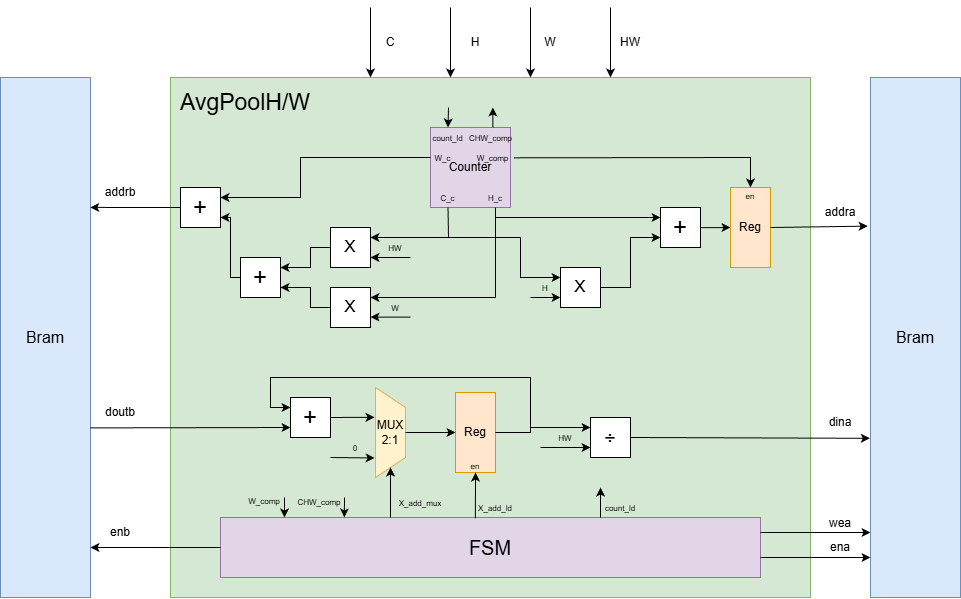
\includegraphics[width=\textwidth]{Image/AvgHW_datapath.png}
    \label{fig:AvgHW_datapath}
\end{figure}

\newpage

\begin{enumerate}
    \setcounter{enumi}{1}
    \item \textbf{FSM}
\end{enumerate}
\begin{figure}[h]{FSM của AvgPoolH và AvgPoolW}
    \centering
    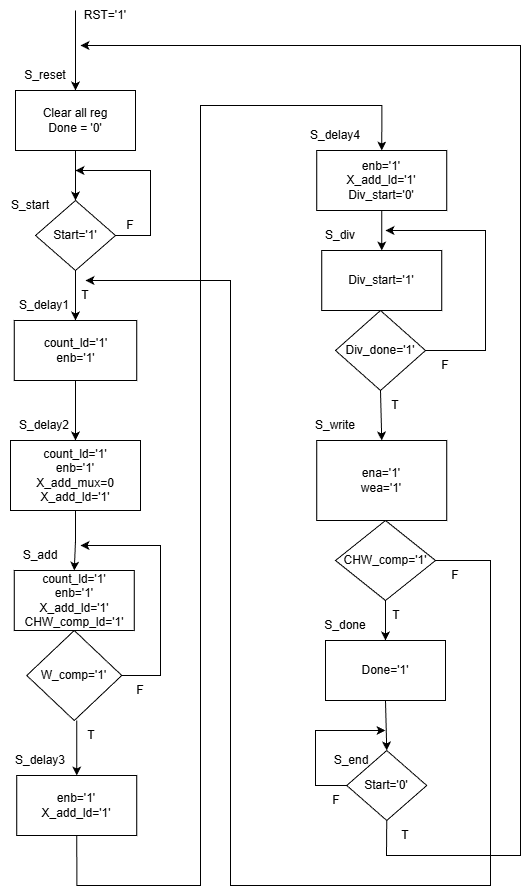
\includegraphics[width=0.55\textwidth]{Image/AvgPoolHW_controller.png}
    \label{fig:AvgPoolHW_FSM}
\end{figure}
\begin{itemize}
    \item FSM gồm 11 trạng thái. \texttt{S\_start} chờ \texttt{Start\_i}.

    \item \texttt{S\_delay1}, \texttt{S\_delay2}: 2 chu kỳ chờ BRAM
    đọc dữ liệu đầu tiên; \texttt{S\_delay2} reset \texttt{X\_add} về 0.

    \item \texttt{S\_add}: cộng dồn từng phần tử, lặp đến khi
    \texttt{W\_comp} (hoặc \texttt{H\_comp}) = '1'.

    \item \texttt{S\_delay3}, \texttt{S\_delay4}: chốt tổng cuối vào
    \texttt{X\_add}, chuẩn bị kích bộ chia.

    \item \texttt{S\_div}: chờ \texttt{Div\_done}. \texttt{S\_write}:
    ghi kết quả, kiểm tra \texttt{CHW\_comp} — nếu chưa xong quay về
    \texttt{S\_delay1} xử lý pixel tiếp theo.

    \item \texttt{S\_done}, \texttt{S\_end}: bật \texttt{Done\_o},
    chờ \texttt{Start\_i} hạ.
\end{itemize}

\newpage

\subsection{AvgPool}
AvgPool tính trung bình cộng toàn bộ mặt phẳng không gian $H \times W$
của mỗi kênh, cho ra đầu ra kích thước $[C, 1, 1]$:
\begin{equation}
    \text{out}[c] = \frac{1}{H \times W}
    \sum_{h=0}^{H-1}\sum_{w=0}^{W-1} \text{input}[c][h][w]
\end{equation}

Cấu trúc FSMD tương tự AvgPoolH/W, với một số điểm khác biệt:

\newpage

Mã giả:
\begin{Verbatim}[frame=single]
Input:
    input[C × H × W]
    C, H, W

Output:
    output[C]

HW = H × W

For C_c = 0 to C - 1:

    X_add = 0

    For H_c = 0 to H - 1:
        For W_c = 0 to W - 1:

            addrb = C_c × HW + H_c × W + W_c
            doutb = input[addrb]

            X_add = X_add + doutb

    Div_out = X_add / HW

    dina = Div_out
    addra = C_c

    output[addra] = dina

Return output
\end{Verbatim}

\newpage

\begin{enumerate}
    \item \textbf{Datapath}
\end{enumerate}

\begin{itemize}
    \item Tín hiệu kết thúc: \texttt{HW\_comp = W\_comp AND H\_comp} báo
    hết một mặt phẳng $H \times W$;
    \texttt{CHW\_comp = HW\_comp AND C\_comp} báo kết thúc toàn bộ.

    \item Thanh ghi tích lũy mở rộng lên \textbf{32-bit} để tránh
    tràn số khi cộng dồn $H \times W$ giá trị Q8.8.

    \item Bộ chia dùng \texttt{Div\_32bit}, số chia là
    $HW \times 256$ (tức $HW \ll 8$) để giữ đúng định dạng Q8.8 ở
    đầu ra. Địa chỉ ghi $\texttt{addra} = \texttt{C\_c}$.
\end{itemize}

\begin{figure}[h]{Datapath của AvgPool}
    \centering
    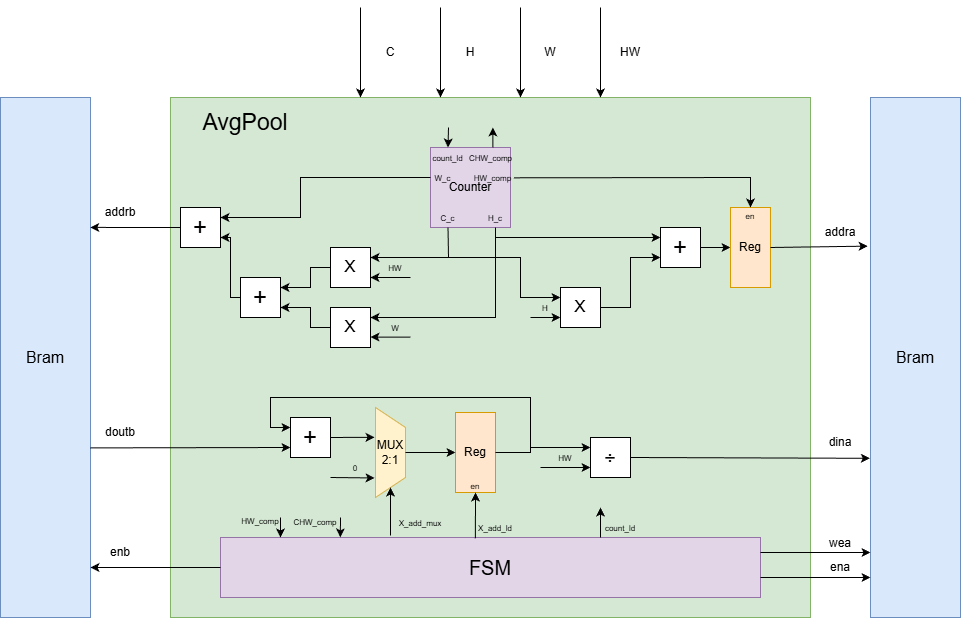
\includegraphics[width=\textwidth]{Image/AvgPool_datapath.png}
    \label{fig:AvgPool_datapath}
\end{figure}

\newpage

\begin{enumerate}
    \setcounter{enumi}{1}
    \item \textbf{FSM}
\end{enumerate}
\begin{figure}[h]{FSM của AvgPool}
    \centering
    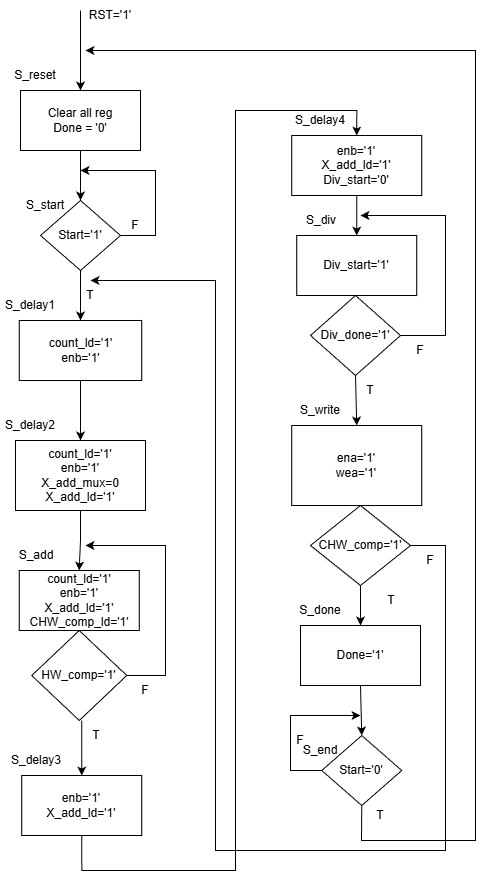
\includegraphics[width=0.55\textwidth]{Image/AvgPool_controller.png}
    \label{fig:AvgPool_FSM}
\end{figure}
\begin{itemize}
    \item FSM có cấu trúc 11 trạng thái giống hệt AvgPoolH/W
    (Hình \ref{fig:AvgPoolHW_FSM}), chỉ thay điều kiện thoát
    \texttt{S\_add} từ \texttt{W\_comp}/\texttt{H\_comp} thành
    \texttt{HW\_comp} — tức vòng lặp trong kết thúc khi cả hai chiều
    H và W đều đã được duyệt hết.
\end{itemize}

\newpage

\section{Các bộ tích chập}
\subsection{Conv1x1}
Bộ tích chập $1\times1$ thực hiện phép biến đổi tuyến tính theo chiều
kênh, không có kernel không gian. Với đầu vào kích thước $[C, N, 1]$
(trong đó $N = H + W$, là kết quả ghép nối pool\_h và pool\_w), mỗi
điểm đầu ra được tính:
\begin{equation}
    \text{out}[oc][n] = \text{bias}[oc] +
    \sum_{ic=0}^{C-1} \text{weight}[oc][ic] \times \text{input}[ic][n]
\end{equation}

Trong đó $oc = 0..C{-}1$ là kênh đầu ra, $ic = 0..C{-}1$ là kênh đầu
vào, $n = 0..N{-}1$ là chỉ số không gian.

Trong thiết kế của nhóm 3: $C = 16$, $H = W = 16$, $N = 32$. Bộ trọng số
gồm $16 \times 16 = 256$ giá trị Q8.8 lưu trong BRAM ROM
(\texttt{bram\_conv1x1\_weight}), bias gồm 16 giá trị
(\texttt{bram\_conv1x1\_bias}).

Mã giả:
\begin{Verbatim}[frame=single]
Input:
    input[C × N]
    weight[C × C]
    bias[C]
    C, H, W

Output:
    output[C × N]

N = H + W

For oc_c = 0 to C - 1:
    For N_c = 0 to N - 1:

        X_add = 0

        For ic_c = 0 to C - 1:

            addrb = ic_c × N + N_c
            doutb = input[addrb]

            weightaddr = oc_c × C + ic_c
            weight_dout = weight[weightaddr]

            Mul_out = doutb × weight_dout

            X_add = X_add + Mul_out

        biasaddr = oc_c
        bias_dout = bias[biasaddr]

        dina = X_add + bias_dout

        addra = oc_c × N + N_c
        output[addra] = dina

Return output
\end{Verbatim}

\begin{enumerate}
    \item \textbf{Datapath}
\end{enumerate}

\begin{figure}[h]{Datapath của Conv1x1}
    \centering
    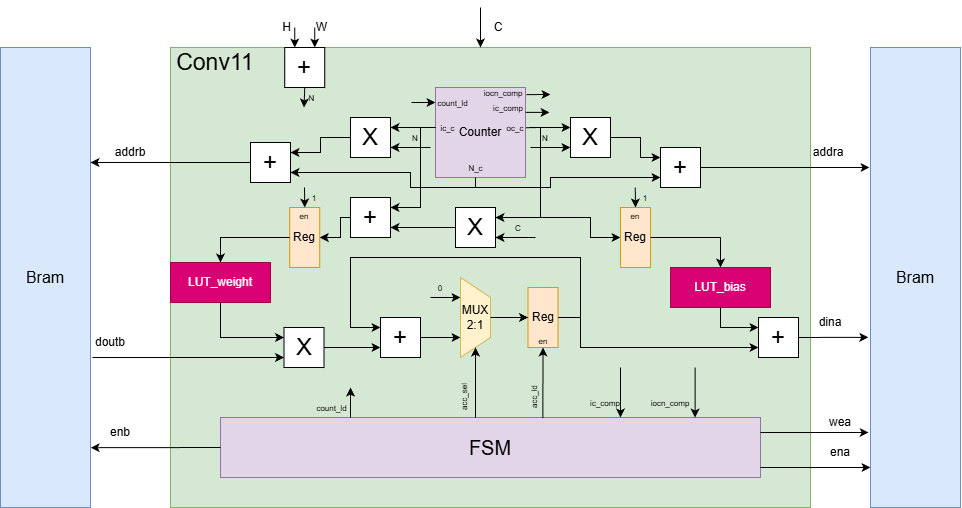
\includegraphics[width=\textwidth]{Image/Conv11_datapath.png}
    \label{fig:Conv11_datapath}
\end{figure}
\begin{itemize}
    \item Tín hiệu kết thúc: \texttt{ic\_comp} báo hết vòng ic, kích tăng
    \texttt{n\_c}; \texttt{iocn\_comp = ic\_comp AND n\_comp AND
    oc\_comp} báo kết thúc toàn bộ.

    \item Địa chỉ đọc BRAM đầu vào:
    $\texttt{addrb} = \texttt{ic\_c} \times N + \texttt{n\_c}$, trong đó $N = H + W$.
    Địa chỉ đọc trọng số:
    $\texttt{weightaddr} = \texttt{oc\_c} \times C + \texttt{ic\_c}$.

    \item Bộ tích lũy MAC 32-bit: bộ nhân \texttt{mul\_16\_noclip}
    nhân \texttt{doutb} với \texttt{weight} ra tích 32-bit, cộng dồn
    vào bộ tích lũy. MUX 2:1 xóa bộ tích lũy về 0 đầu mỗi điểm
    đầu ra.

    \item Kết quả cuối: cắt lấy 16 bit giữa của bộ tích lũy
    (dịch phải 8 bit từ Q16.16 về Q8.8), cộng bias ra \texttt{dina}
    ghi vào BRAM đầu ra.

    \item Địa chỉ ghi đầu ra:
    $\texttt{addra} = \texttt{oc\_c} \times N + \texttt{n\_c}$, được chốt vào thanh ghi
    khi \texttt{ic\_comp = '1'} (kết thúc tích lũy một điểm).

    \item Địa chỉ đọc bias: \texttt{biasaddr} được nạp từ \texttt{oc\_c}
    khi kết thúc tích lũy một điểm, đảm bảo bias sẵn sàng đúng lúc
    ghi kết quả.
\end{itemize}

\begin{enumerate}
    \setcounter{enumi}{1}
    \item \textbf{FSM}
\end{enumerate}
\begin{figure}[h]{FSM của Conv1x1}
    \centering
    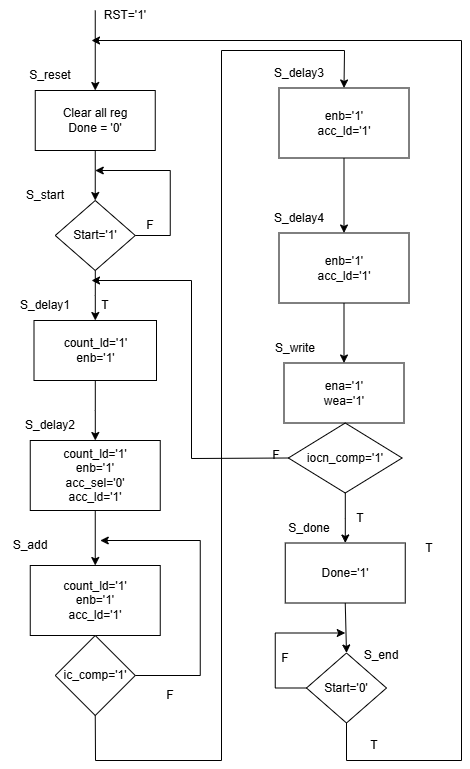
\includegraphics[width=0.55\textwidth]{Image/Conv11_controller.png}
    \label{fig:Conv11_FSM}
\end{figure}
\begin{itemize}
    \item FSM gồm 10 trạng thái. \texttt{S\_start} chờ
    \texttt{Start\_i = '1'}.

    \item \texttt{S\_delay1}, \texttt{S\_delay2}: 2 chu kỳ chờ BRAM
    trả dữ liệu. \texttt{S\_delay2} xóa bộ tích lũy về 0
    (\texttt{acc\_sel = '0'}).

    \item \texttt{S\_add}: cộng dồn tích $\text{weight} \times
    \text{input}$ vào bộ tích lũy, lặp đến khi \texttt{ic\_comp = '1'}
    (hết $C$ kênh đầu vào).

    \item \texttt{S\_delay3}, \texttt{S\_delay4}: 2 chu kỳ chốt giá trị
    tích lũy cuối cùng vào bộ tích lũy (do BRAM và bộ nhân có trễ
    pipeline).

    \item \texttt{S\_write}: bật \texttt{ena}, \texttt{wea} ghi kết quả
    ra BRAM đầu ra, đồng thời nạp \texttt{bias\_ld}. Kiểm tra
    \texttt{iocn\_comp}: nếu chưa xong quay về \texttt{S\_delay1}
    tính điểm tiếp theo; nếu xong chuyển sang \texttt{S\_done}.

    \item \texttt{S\_done}, \texttt{S\_end}: bật \texttt{Done\_o = '1'},
    chờ \texttt{Start\_i} hạ xuống '0' rồi quay về \texttt{S\_reset}.
\end{itemize}

So với các bộ AvgPool, Conv1x1 không cần bộ chia vì phép tích chập
$1\times1$ chỉ gồm nhân--tích lũy--cộng bias, nên FSM đơn giản hơn
(không có trạng thái \texttt{S\_div}).

\subsection{Conv3x3}
Bộ tích chập $3\times3$ là thành phần tính toán nặng nhất trong mô-đun
EMA. Với kernel $3\times3$ và padding ``same'', mỗi điểm đầu ra được
tính:
\begin{equation}
    \text{out}[oc][oh][ow] = \text{bias}[oc] +
    \sum_{ic=0}^{C-1}\sum_{ky=0}^{2}\sum_{kx=0}^{2}
    \text{weight}[oc][ic][ky][kx] \times \text{input}[ic][oh{+}ky{-}1][ow{+}kx{-}1]
\end{equation}

Trong đó $oc = 0..C{-}1$ là kênh đầu ra, $oh = 0..H{-}1$ và
$ow = 0..W{-}1$ là tọa độ không gian, $ic = 0..C{-}1$ là kênh đầu
vào, $ky, kx = 0..2$ là vị trí kernel.

Tại giai đoạn 3: $C = 16$, $H = W = 16$. Bộ trọng số gồm
$16 \times 16 \times 3 \times 3 = 2304$ giá trị Q8.8 lưu trong 9 bản
sao BRAM ROM (\texttt{bram\_conv3x3\_weight}), bias gồm 16 giá trị
(\texttt{bram\_conv3x3\_bias}).

Datapath của Conv3x3 được chia thành hai khối chức năng:
\textbf{Conv33\_address} (tính địa chỉ và padding) và
\textbf{Conv33\_calc} (nhân--cộng--tích lũy).

Mã giả:
\begin{Verbatim}[frame=single]
Input:
    input[C * H * W]
    weight[C * C * 9]
    bias[C]
    C, H, W

Output:
    output[C * H * W]

HW = H * W

For oc_c = 0 to C - 1:

    biasaddr = oc_c
    bias_dout = bias[biasaddr]

    For oh_c = 0 to H - 1:
        For ow_c = 0 to W - 1:

            X_add = 0

            For ic_c = 0 to C - 1:

                base = ic_c * HW + oh_c * W + ow_c

                addrb0 = base - W - 1
                addrb1 = base - W
                addrb2 = base - W + 1
                addrb3 = base - 1
                addrb4 = base
                addrb5 = base + 1
                addrb6 = base + W - 1
                addrb7 = base + W
                addrb8 = base + W + 1

                If oh_c == 0 or ow_c == 0:
                    doutb0 = 0
                Else:
                    doutb0 = input[addrb0]

                If oh_c == 0:
                    doutb1 = 0
                Else:
                    doutb1 = input[addrb1]

                If oh_c == 0 or ow_c == W - 1:
                    doutb2 = 0
                Else:
                    doutb2 = input[addrb2]

                If ow_c == 0:
                    doutb3 = 0
                Else:
                    doutb3 = input[addrb3]

                doutb4 = input[addrb4]

                If ow_c == W - 1:
                    doutb5 = 0
                Else:
                    doutb5 = input[addrb5]

                If oh_c == H - 1 or ow_c == 0:
                    doutb6 = 0
                Else:
                    doutb6 = input[addrb6]

                If oh_c == H - 1:
                    doutb7 = 0
                Else:
                    doutb7 = input[addrb7]

                If oh_c == H - 1 or ow_c == W - 1:
                    doutb8 = 0
                Else:
                    doutb8 = input[addrb8]

                weightaddr_base = oc_c * C * 9 + ic_c * 9

                weightaddr0 = weightaddr_base + 0
                weightaddr1 = weightaddr_base + 1
                weightaddr2 = weightaddr_base + 2
                weightaddr3 = weightaddr_base + 3
                weightaddr4 = weightaddr_base + 4
                weightaddr5 = weightaddr_base + 5
                weightaddr6 = weightaddr_base + 6
                weightaddr7 = weightaddr_base + 7
                weightaddr8 = weightaddr_base + 8

                Mul_out0 = doutb0 * weight[weightaddr0]
                Mul_out1 = doutb1 * weight[weightaddr1]
                Mul_out2 = doutb2 * weight[weightaddr2]
                Mul_out3 = doutb3 * weight[weightaddr3]
                Mul_out4 = doutb4 * weight[weightaddr4]
                Mul_out5 = doutb5 * weight[weightaddr5]
                Mul_out6 = doutb6 * weight[weightaddr6]
                Mul_out7 = doutb7 * weight[weightaddr7]
                Mul_out8 = doutb8 * weight[weightaddr8]

                X_add = X_add
                      + Mul_out0 + Mul_out1 + Mul_out2
                      + Mul_out3 + Mul_out4 + Mul_out5
                      + Mul_out6 + Mul_out7 + Mul_out8

            dina = X_add + bias_dout

            addra = oc_c * HW + oh_c * W + ow_c
            output[addra] = dina

Return output
\end{Verbatim}

\begin{enumerate}
    \item \textbf{Datapath tổng quan}
\end{enumerate}

\begin{itemize}
    \item Đầu vào được lưu trong \textbf{9 BRAM} chứa cùng một bản
    dữ liệu, mỗi BRAM cung cấp một giá trị \texttt{doutb0..8}
    tương ứng với 9 vị trí láng giềng. Khối \texttt{Conv33\_address}
    sinh ra 9 địa chỉ đọc \texttt{addrb0..8} và 9 địa chỉ trọng số
    \texttt{weightaddr0..8} cùng lúc, đồng thời xuất vector
    \texttt{cond[8:0]} cho biết vị trí nào nằm ngoài biên (cần
    zero-padding).

    \item \textbf{9 bản sao} \texttt{bram\_conv3x3\_weight} nhận
    \texttt{weightaddr0..8}, trả về 9 trọng số song song.
    \texttt{LUT\_bias} cung cấp bias theo \texttt{biasaddr}.

    \item Khối \texttt{Conv33\_calc} nhận 9 cặp
    $(\text{doutb}, \text{weight})$, thực hiện nhân--cộng--tích lũy
    rồi xuất \texttt{dina} ghi vào BRAM đầu ra qua cổng
    \texttt{addra}.

    \item FSM điều khiển chung các tín hiệu nạp bộ đếm, reset
    bộ tích lũy, cho phép đọc/ghi BRAM cho cả hai khối.
\end{itemize}

\begin{figure}[h]{Cấu trúc top-level của Conv3x3}
    \centering
    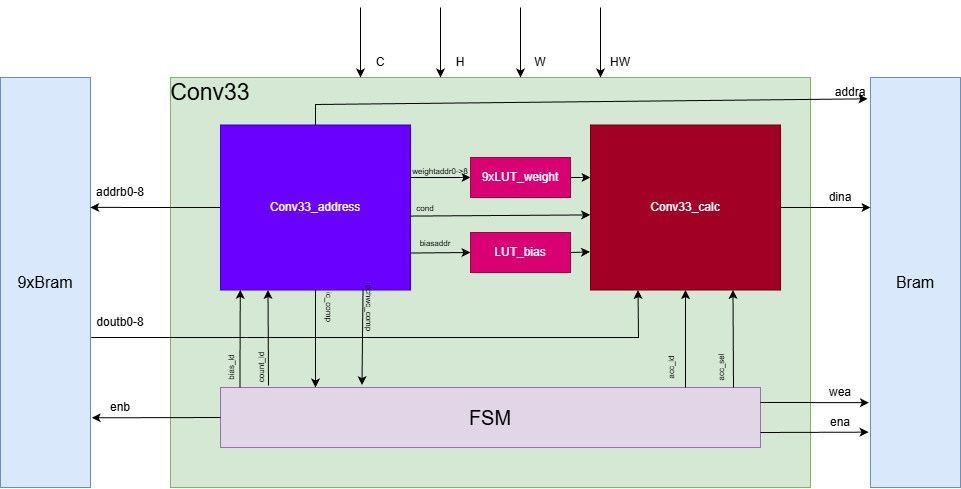
\includegraphics[width=0.9\textwidth]{Image/Conv33_top.png}
    \label{fig:Conv33_top}
\end{figure}

\newpage

\begin{enumerate}
    \setcounter{enumi}{1}
    \item \textbf{Khối Conv33\_address}
\end{enumerate}
\begin{figure}[h]{Datapath khối tính địa chỉ Conv33\_address}
    \centering
    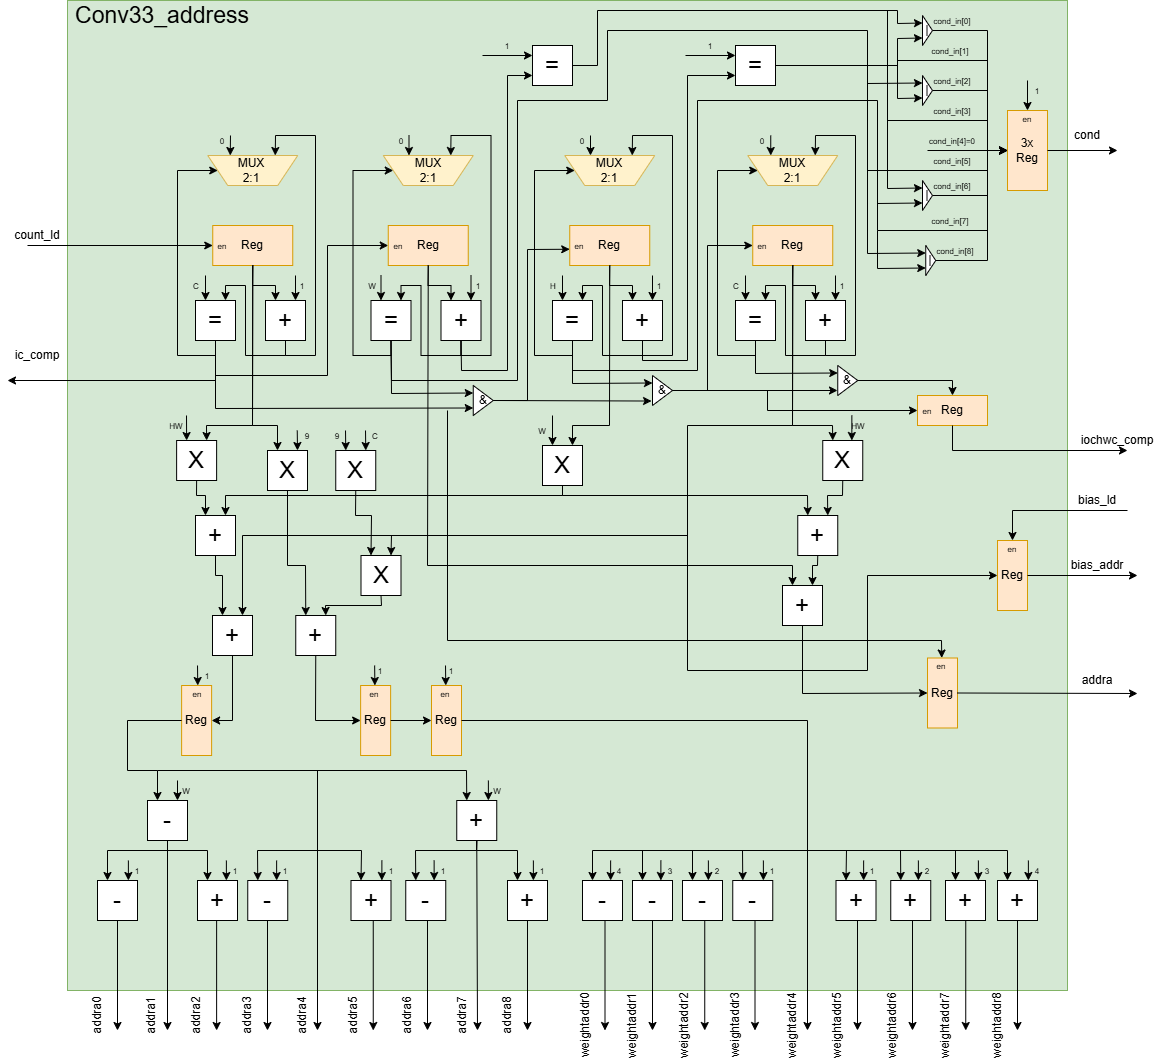
\includegraphics[width=\textwidth]{Image/Conv33_address.png}
    \label{fig:Conv33_address}
\end{figure}
\begin{itemize}
    \item Tín hiệu kết thúc: \texttt{ic\_comp} báo hết vòng ic, kích tăng
    \texttt{ow\_c}; \texttt{icowhc\_comp = ic\_comp AND ow\_comp AND
    oh\_comp AND oc\_comp} báo kết thúc toàn bộ.

    \item Địa chỉ trung tâm (vị trí kernel $(1,1)$):
    $\texttt{ic\_c} \times HW + \texttt{oh\_c} \times W + \texttt{ow\_c}$, được
    chốt qua thanh ghi. Từ địa chỉ trung tâm, tính thêm $\pm W$
    (hàng trên/dưới). Chín địa chỉ đầu vào được tính đồng thời bằng
    $\pm 1$ từ ba giá trị gốc:
    \begin{equation}
    \begin{bmatrix}
        \text{sub}{-}1 & \text{sub} & \text{sub}{+}1 \\
        \text{base}{-}1 & \text{base} & \text{base}{+}1 \\
        \text{add}{-}1 & \text{add} & \text{add}{+}1
    \end{bmatrix}
    \end{equation}

    \item Địa chỉ trọng số:
    $\texttt{weightaddr} = \texttt{oc\_c} \times C \times 9 + \texttt{ic\_c} \times 9$,
    qua \textbf{2 thanh ghi} pipeline trước khi vào BRAM để đồng bộ
    với trễ đọc. Chín địa chỉ weight tính bằng cách cộng offset
    $0..8$ vào \texttt{weightaddr}.

    \item \textbf{Zero-padding}: vector \texttt{cond[8:0]} xác định
    vị trí nào nằm ngoài biên. Mỗi bit được tính tổ hợp từ các tín
    hiệu biên của \texttt{ow\_c} và \texttt{oh\_c} (so sánh với 0 và
    giá trị max). Vector \texttt{cond} đi qua \textbf{3 thanh ghi}
    pipeline để đồng bộ chính xác với dữ liệu \texttt{doutb} từ BRAM.

    \item Địa chỉ ghi đầu ra:
    $\texttt{addra} = \texttt{oc\_c} \times HW + \texttt{oh\_c} \times W + \texttt{ow\_c}$,
    chốt vào thanh ghi khi \texttt{ic\_comp = '1'}.

    \item Địa chỉ bias: \texttt{biasaddr} nạp từ \texttt{oc\_c} khi
    kết thúc tích lũy một pixel.
\end{itemize}

\begin{enumerate}
    \setcounter{enumi}{2}
    \item \textbf{Khối Conv33\_calc}
\end{enumerate}

\begin{figure}[h]{Datapath khối tính toán Conv33\_calc}
    \centering
    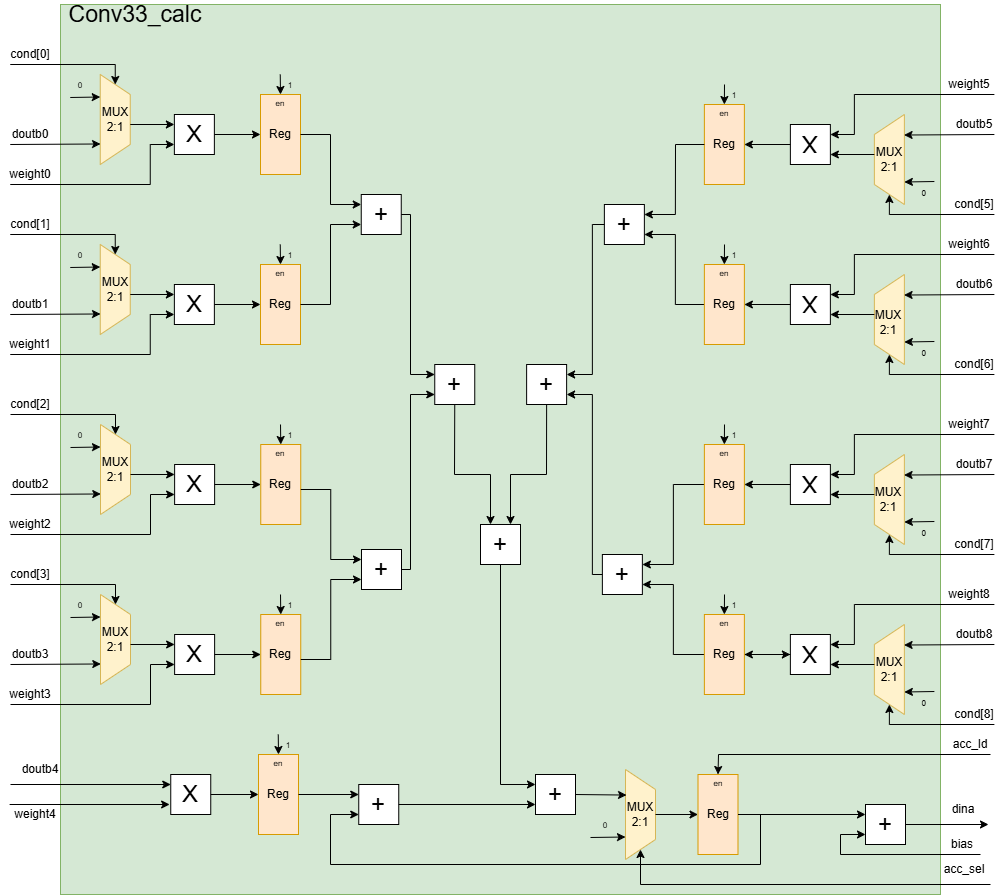
\includegraphics[width=\textwidth]{Image/Conv33_calc.png}
    \label{fig:Conv33_calc}
\end{figure}

\begin{itemize}
    \item Với 8 vị trí biên (0--3 và 5--8), MUX 2:1 chọn giữa
    \texttt{doutb} thật và $0$ dựa trên \texttt{cond[i]}: nếu
    \texttt{cond[i] = '1'} (ngoài biên), đầu vào nhân bị ép về 0.
    Vị trí trung tâm (4) luôn hợp lệ, không cần MUX.

    \item \textbf{9 bộ nhân} \texttt{mul\_16\_noclip} thực hiện song
    song: $\text{Mul}_i = \texttt{doutb}_i \times \texttt{weight}_i$
    ($i = 0..8$), kết quả 32-bit, chốt qua thanh ghi.

    \item \textbf{Cây cộng 4 tầng} gộp 9 tích thành một tổng duy nhất.
    Tầng 1 gộp thành 4 cặp, tầng 2 gộp thành 2, tầng 3--4 cộng nốt
    với giá trị bộ tích lũy cũ. Tổng 9 tích cộng luôn với bộ tích lũy
    trong cùng chu kỳ, nên mỗi bước \texttt{ic\_c} hoàn thành
    $9$ phép MAC.

    \item \textbf{Thanh ghi tích lũy} (32-bit): MUX 2:1 reset về
    $0$ đầu mỗi pixel đầu ra. Sau khi lặp hết $C$ kênh đầu vào,
    bộ tích lũy chứa tổng $C \times 9 = 144$ phép MAC.

    \item Kết quả cuối: cắt lấy 16 bit giữa của bộ tích lũy (dịch
    phải 8 bit từ Q16.16 về Q8.8) cộng bias ra \texttt{dina}.
\end{itemize}

\newpage

\begin{enumerate}
    \setcounter{enumi}{3}
    \item \textbf{FSM}
\end{enumerate}

\begin{figure}[h]{FSM của Conv3x3}
    \centering
    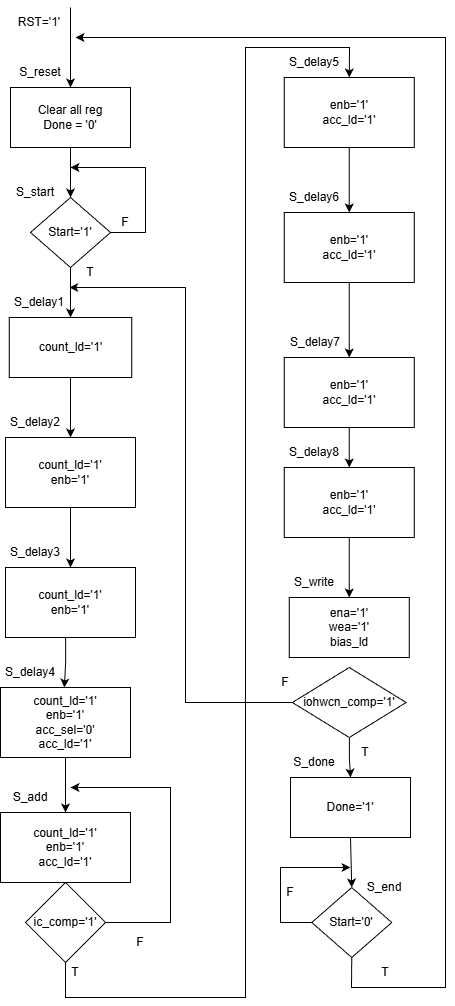
\includegraphics[width=0.45\textwidth]{Image/Conv33_controller.png}
    \label{fig:Conv33_FSM}
\end{figure}
\begin{itemize}
    \item FSM gồm 14 trạng thái. \texttt{S\_start} chờ
    \texttt{Start\_i = '1'}.

    \item \texttt{S\_delay1} $\to$ \texttt{S\_delay4}: 4 chu kỳ
    khởi tạo pipeline — bao gồm 2 chu kỳ trễ đọc BRAM, 1 chu kỳ
    pipeline thanh ghi bộ nhân, và 1 chu kỳ cho vector
    \texttt{pad\_mask} ổn định (3 tầng thanh ghi). Tại
    \texttt{S\_delay4}, bộ tích lũy được reset về 0
    (\texttt{acc\_sel = '0'}).

    \item \texttt{S\_add}: cộng dồn 9 tích vào bộ tích lũy mỗi chu kỳ,
    lặp đến khi \texttt{ic\_comp = '1'} (hết $C$ kênh đầu vào).

    \item \texttt{S\_delay5} $\to$ \texttt{S\_delay8}: 4 chu kỳ
    ``xả pipeline'' — các tích và tổng còn nằm trong thanh ghi pipeline
    cần thời gian truyền qua cây cộng và chốt vào bộ tích lũy.

    \item \texttt{S\_write}: bật \texttt{ena}, \texttt{wea},
    \texttt{bias\_ld}; ghi kết quả ra BRAM đầu ra. Kiểm tra
    \texttt{icowhc\_comp}: nếu chưa xong quay về \texttt{S\_delay1}
    tính pixel tiếp; nếu xong chuyển sang \texttt{S\_done}.

    \item \texttt{S\_done}, \texttt{S\_end}: bật \texttt{Done\_o = '1'},
    chờ \texttt{Start\_i} hạ.
\end{itemize}

So với Conv1x1, Conv3x3 có ba điểm khác biệt chính: (1) vòng lặp bốn
tầng thay vì ba tầng (thêm chiều oh, ow); (2) 9 bộ nhân và 9 BRAM song
song thay vì 1; (3) pipeline sâu hơn (4 chu kỳ delay thay vì 2) do
thêm thanh ghi cho trọng số và vector padding.

\section{Chuẩn hóa và kích hoạt}
\subsection{GroupNorm}
Group Normalization chuẩn hóa từng kênh trên toàn bộ mặt phẳng không
gian $H \times W$. Với mỗi kênh $c$, phép tính gồm bốn bước:
\begin{equation}
    \mu_c = \frac{1}{HW}\sum_{h,w} x[c][h][w], \qquad
    \sigma^2_c = \frac{1}{HW}\sum_{h,w} (x[c][h][w] - \mu_c)^2
\end{equation}
\begin{equation}
    \hat{x}[c][h][w] = \frac{x[c][h][w] - \mu_c}{\sqrt{\sigma^2_c + \varepsilon}},
    \qquad
    y[c][h][w] = \gamma_c \cdot \hat{x}[c][h][w] + \beta_c
\end{equation}

Tại giai đoạn 3: $C = 16$, $H = W = 16$, $HW = 256$, $\varepsilon = 1$
(dưới dạng Q8.8, giá trị nhỏ tránh chia cho 0). Tham số $\gamma$ và
$\beta$ (mỗi loại 16 giá trị Q8.8) lưu trong \texttt{bram\_gn\_weight}
và \texttt{bram\_gn\_bias}.

Khác với các mô-đun trước, GroupNorm xử lý \textbf{tuần tự theo từng
kênh}: hoàn thành cả 4 bước cho kênh $c$ rồi mới chuyển sang kênh
$c{+}1$:

Mã giả
\begin{Verbatim}[frame=single]
Input:
    input[C * H * W]
    gamma[C]
    beta[C]
    C, H, W

Output:
    output[C * H * W]

HW = H * W
eps = b00000001

For C_c = 0 to C - 1:

    X_add = 0

    For H_c = 0 to H - 1:
        For W_c = 0 to W - 1:

            addrb = C_c * HW + H_c * W + W_c
            doutb = input[addrb]

            X_add = X_add + doutb

    mean = X_add / HW


    X_square_add = 0

    For H_c = 0 to H - 1:
        For W_c = 0 to W - 1:

            addrb = C_c * HW + H_c * W + W_c
            doutb = input[addrb]

            X_sub = doutb - mean
            Mul_out = X_sub * X_sub

            X_square_add = X_square_add + Mul_out

    variance = X_square_add / HW


    Sqrt_in = variance + eps
    Sqrt_out = sqrt(Sqrt_in)

    Inv_std = 0x0100 / Sqrt_out


    gammaaddr = C_c
    betaaddr = C_c

    gamma_dout = gamma[gammaaddr]
    beta_dout = beta[betaaddr]

    For H_c = 0 to H - 1:
        For W_c = 0 to W - 1:

            addrb = C_c * HW + H_c * W + W_c
            doutb = input[addrb]

            X_sub = doutb - mean
            X_norm = X_sub * Inv_std

            Mul_out = X_norm * gamma_dout
            dina = Mul_out + beta_dout

            addra = C_c * HW + H_c * W + W_c
            output[addra] = dina

Return output
\end{Verbatim}

\begin{enumerate}
    \item \textbf{Datapath}
\end{enumerate}

\begin{figure}[h]{Datapath của GroupNorm}
    \centering
    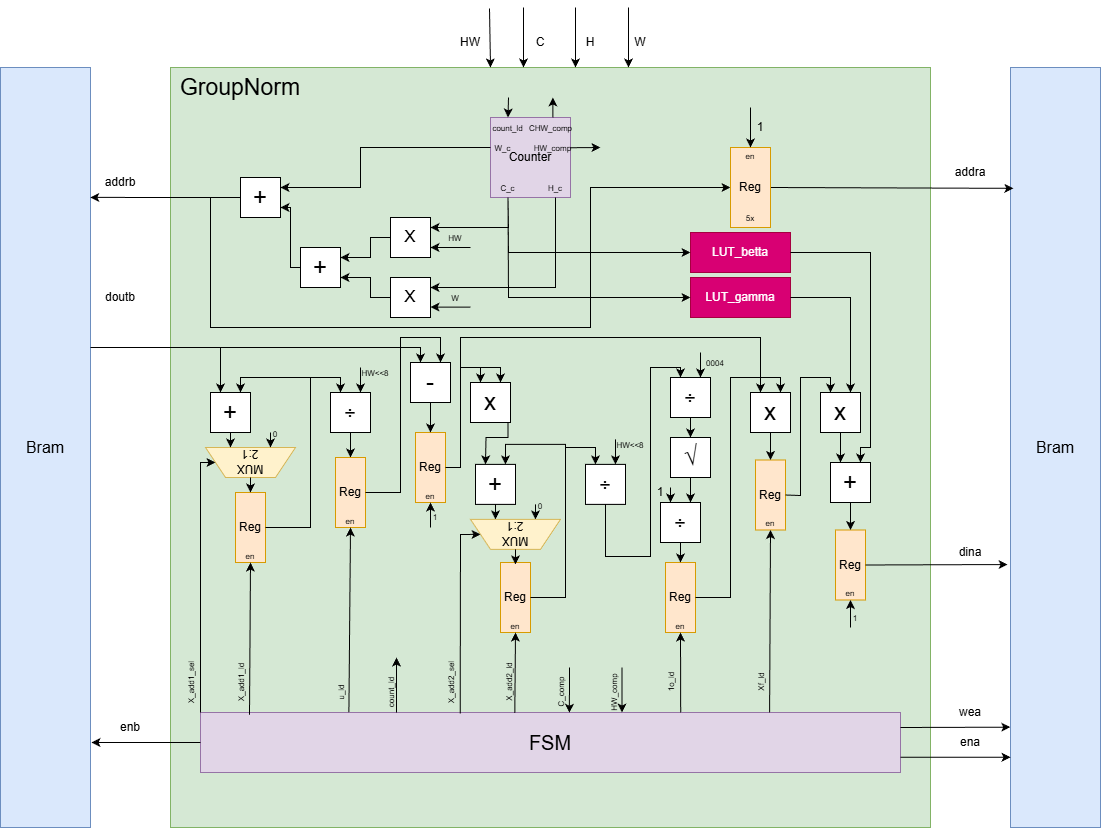
\includegraphics[width=0.9\textwidth]{Image/GroupNorm_datapath.png}
    \label{fig:GroupNorm_datapath}
\end{figure}

\begin{itemize}
    \item \textbf{Khối tính địa chỉ}: dùng chung cho cả đọc và ghi.
    $\texttt{addrb} = \texttt{C\_c} \times HW + \texttt{H\_c} \times W + \texttt{W\_c}$.
    Địa chỉ ghi \texttt{addra} đi qua \textbf{5 thanh ghi} pipeline
    để đồng bộ với trễ tính toán affine. Hai bảng LUT đọc
    $\gamma_c$, $\beta_c$ theo \texttt{C\_c}.

    \item \textbf{Tính mean ($\mu$)}: thanh ghi tích lũy 32-bit cộng
    dồn \texttt{doutb} (mở rộng dấu lên 32-bit) qua $HW$ phần tử.
    MUX 2:1 reset về 0 đầu mỗi kênh. Sau khi cộng xong, bộ chia
    \texttt{Div\_32bit} chia tổng cho $HW \times 256$ (tức $HW \ll 8$)
    ra giá trị $\mu$ (Q8.8), chốt vào thanh ghi.

    \item \textbf{Tính variance ($\sigma^2$)}: duyệt lại $HW$ phần tử
    lần thứ hai. Mỗi phần tử tính $(\texttt{doutb} - \mu)$, rồi bình
    phương bằng bộ nhân (nhân chính nó với chính nó). Thanh ghi tích
    lũy 32-bit cộng dồn các tích. Bộ chia \texttt{Div\_32bit} thứ hai
    chia tổng cho $HW \ll 8$ ra $\sigma^2$ (Q8.8).

    \item \textbf{Tính inv\_std ($1/\sigma$)}: cộng $\varepsilon = 1$
    vào $\sigma^2$ ra $\sigma^2 + \varepsilon$. Bộ \texttt{SQRT} tính
    $\sigma = \sqrt{\sigma^2 + \varepsilon}$. Bộ chia
    \texttt{Div\_16bit} chia $1.0$ (= \texttt{0x0100} trong Q8.8) cho
    $\sigma$ ra nghịch đảo độ lệch chuẩn $1/\sigma$, chốt vào
    thanh ghi.

    \item \textbf{Affine transform}: duyệt $HW$ phần tử lần thứ ba.
    Mỗi phần tử tính:
    \begin{itemize}
        \item $\hat{x} = (x - \mu) \times (1/\sigma)$ — bộ nhân
        Booth--Wallace thứ nhất
        \item $y = \hat{x} \times \gamma + \beta$ — bộ nhân
        Booth--Wallace thứ hai, cộng $\beta$ rồi ghi vào BRAM đầu ra
    \end{itemize}
\end{itemize}

\begin{enumerate}
    \setcounter{enumi}{1}
    \item \textbf{FSM}
\end{enumerate}
\begin{itemize}
    \item FSM gồm 32 trạng thái, chia thành 5 giai đoạn chính cho mỗi
    kênh:

    \item \textbf{Giai đoạn 1 — Tính mean}: \texttt{S\_delay1},
    \texttt{S\_delay2} khởi tạo pipeline và reset \texttt{X\_add1} về
    0. \texttt{S\_add1} cộng dồn đến khi \texttt{HW\_comp = '1'}.
    \texttt{S\_delay3}, \texttt{S\_delay4} chốt giá trị cuối.
    \texttt{S\_div1} chờ \texttt{Div\_done1}. \texttt{S\_delay5} chốt
    $\mu$ vào thanh ghi $u$.

    \item \textbf{Giai đoạn 2 — Tính variance}:
    \texttt{S\_delay6..S\_delay6b} (3 chu kỳ) khởi động lại bộ đếm và
    pipeline cho lượt duyệt thứ hai. \texttt{S\_delay7} reset
    \texttt{X\_add2} về 0. \texttt{S\_add2} cộng dồn $(x - \mu)^2$.
    \texttt{S\_delay8..S\_delay10} (5 chu kỳ) xả pipeline. \texttt{S\_div2}
    chờ bộ chia variance.

    \item \textbf{Giai đoạn 3 — Tính inv\_std}: \texttt{S\_sqrt} chờ
    $\sqrt{\sigma^2 + \varepsilon}$. \texttt{S\_div3} chờ phép chia
    $1/\sigma$. \texttt{S\_delay11} chốt $ro = 1/\sigma$.

    \item \textbf{Giai đoạn 4 — Affine transform}:
    \texttt{S\_delay12..S\_delay15} (4 chu kỳ) khởi động pipeline lượt
    duyệt thứ ba. \texttt{S\_write} ghi kết quả affine ra BRAM đầu ra,
    bật \texttt{ena} và \texttt{wea}, lặp đến khi \texttt{HW\_comp = '1'}.

    \item \textbf{Giai đoạn 5 — Xả pipeline ghi}:
    \texttt{S\_delay16..S\_delay20} (5 chu kỳ) tiếp tục ghi các giá trị
    còn trong pipeline, \texttt{ena} và \texttt{wea} vẫn bật. Tại
    \texttt{S\_delay20}, kiểm tra \texttt{C\_comp}: nếu chưa hết $C$
    kênh, tăng \texttt{C\_c} và quay về \texttt{S\_delay1}; nếu xong
    chuyển sang \texttt{S\_done}.

    \item \texttt{S\_done}, \texttt{S\_end}: bật \texttt{Done\_o = '1'},
    chờ \texttt{Start\_i} hạ.
\end{itemize}

\begin{figure}[h]{FSM của GroupNorm}
    \centering
    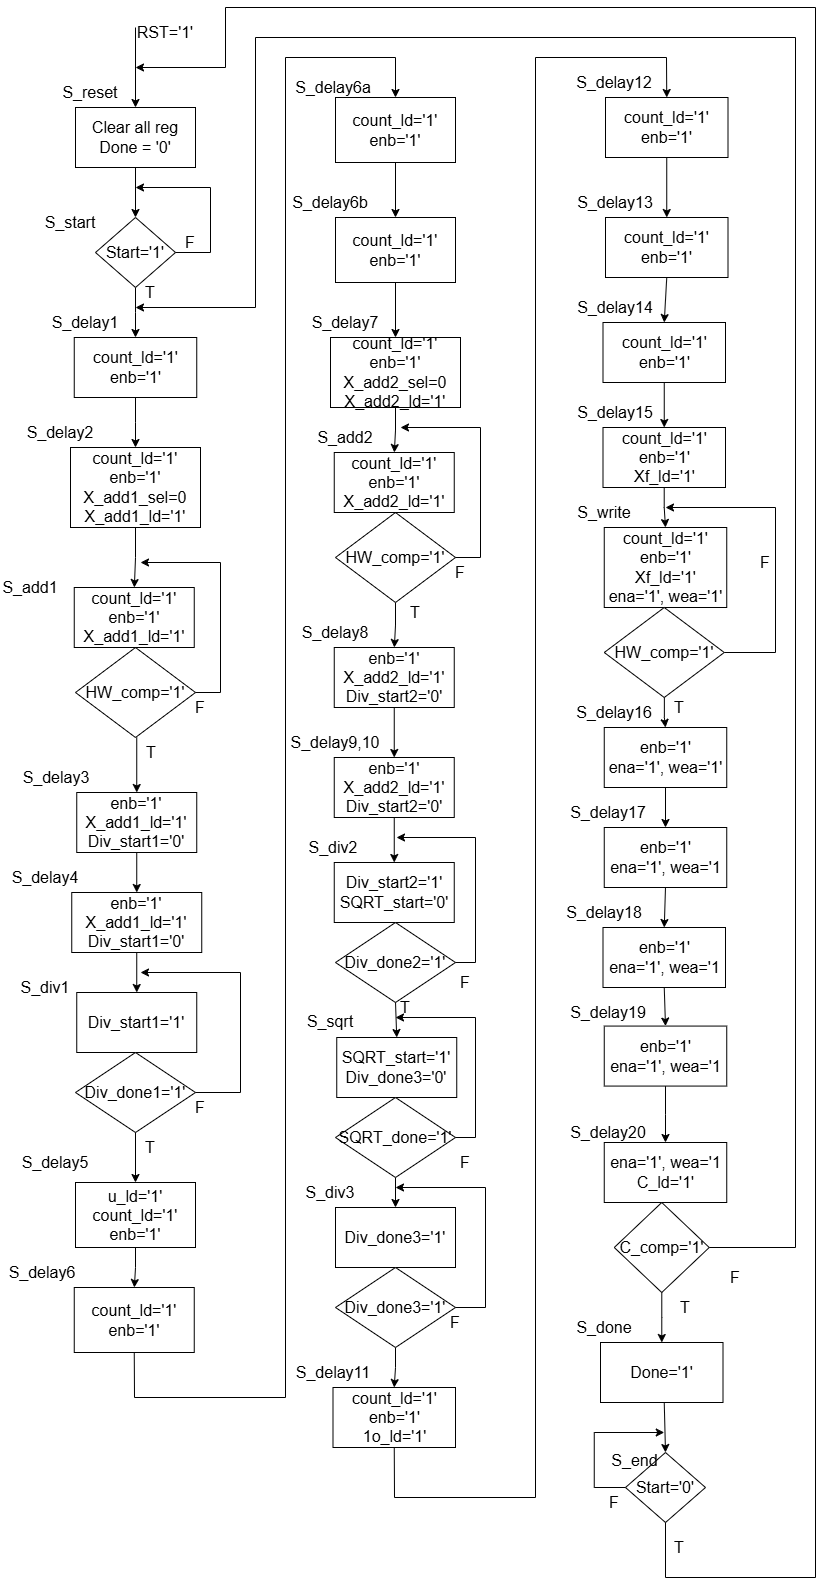
\includegraphics[width=0.55\textwidth]{Image/GroupNorm_controller.png}
    \label{fig:GroupNorm_FSM}
\end{figure}

GroupNorm là mô-đun phức tạp nhất trong thiết kế: mỗi kênh cần duyệt
dữ liệu 3 lượt (mean, variance, affine) và gọi 3 bộ chia cùng 1 bộ
SQRT tuần tự. Tổng thời gian xử lý mỗi kênh phụ thuộc chủ yếu vào
$HW$ và độ trễ của các bộ chia/SQRT.

\subsection{Sigmoid}
Sigmoid áp hàm sigmoid lên toàn bộ bản đồ đặc trưng kích thước
$[C, H, W]$, xử lý từng phần tử:
\begin{equation}
    y[c][h][w] = \sigma\bigl(x[c][h][w]\bigr)
    = \frac{1}{1 + e^{-x}}
\end{equation}

Khác với các mô-đun trước sử dụng FSM đa trạng thái với các bước tuần
tự, Sigmoid áp dụng kiến trúc \textbf{pipeline hoàn toàn}: bộ
\texttt{exp\_continuos} và \texttt{Div\_16bit\_continuos} đều là các
khối tổ hợp nhiều tầng thanh ghi, có thể nhận đầu vào mới mỗi chu kỳ
mà không cần chờ kết quả trước đó. Nhờ vậy, sau giai đoạn khởi tạo
ban đầu, mô-đun xuất một kết quả sigmoid mỗi chu kỳ xung nhịp.

Tại giai đoạn 3: $C = 16$, $H = W = 16$, tổng $C \times N = C \times (H + W)
= 512$ phần tử.

Mã giả:
\begin{Verbatim}[frame=single]
Input:
    input[C * N]
    C, H, W

Output:
    output[C * N]

N = H + W

For C_c = 0 to C - 1:
    For N_c = 0 to N - 1:

        addrb = C_c * N + N_c
        doutb = input[addrb]

        Exp_out = exp(-doutb)

        Div_in = 1 + Exp_out
        Div_out = 1 / Div_in

        dina = Div_out
        addra = C_c * N + N_c

        output[addra] = dina

Return output
\end{Verbatim}

\begin{enumerate}
    \item \textbf{Datapath}
\end{enumerate}
\begin{figure}[h]{Datapath của Sigmoid}
    \centering
    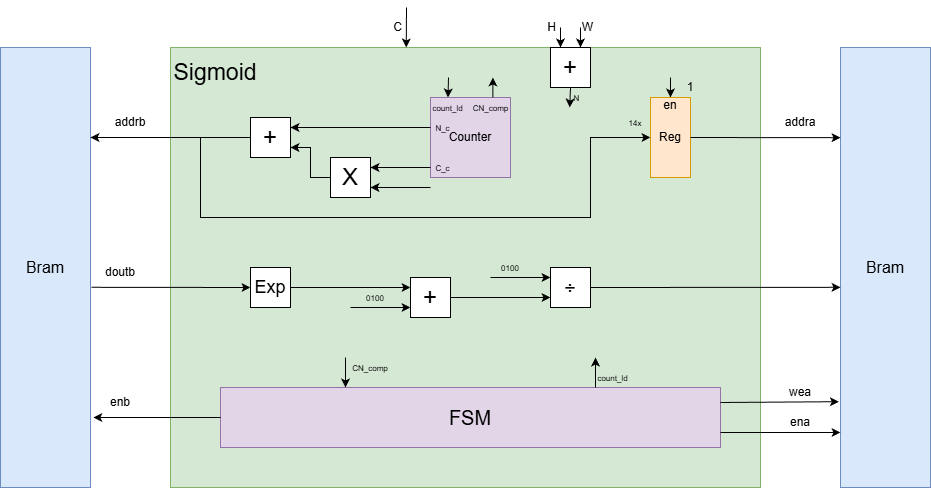
\includegraphics[width=\textwidth]{Image/Sigmoid_datapath.png}
    \label{fig:Sigmoid_datapath}
\end{figure}
\begin{itemize}
    \item Tín hiệu kết thúc: \texttt{CN\_comp = N\_comp AND C\_comp}.
    Bộ đếm chạy liên tục, mỗi chu kỳ tăng \texttt{N\_c} lên 1.

    \item \textbf{Địa chỉ đọc}: $\texttt{addrb} = \texttt{C\_c} \times N + \texttt{N\_c}$,
    dùng bộ nhân và bộ cộng. Dữ liệu \texttt{doutb}
    có sẵn sau 2 chu kỳ trễ BRAM.
    \item \textbf{Pipeline tính toán} gồm hai tầng nối tiếp:
    \begin{itemize}
        \item \texttt{exp\_continuos}: tính $e^x$ qua 3 bảng LUT
        (phần nguyên, phần thập phân cao, phần thập phân thấp), chọn
        giữa LUT dương/âm theo bit dấu, rồi nhân 3 tầng
        Booth--Wallace pipeline.
        Tổng trễ: \textbf{4 chu kỳ} (1 thanh ghi đầu vào + 1 thanh
        ghi LUT + 2 thanh ghi nhân).

        \item Phép cộng $1 + e^{-x}$: tổ hợp thuần, cộng
        \texttt{0x0100} (= 1.0 trong Q8.8) vào kết quả exp.

        \item \texttt{Div\_16bit\_continuos}: chia $1.0$ cho
        $(1 + e^{-x})$ bằng thuật toán Goldschmidt pipeline —
        chuẩn hóa số chia qua barrel shifter, sau đó 3 vòng lặp
        Goldschmidt (mỗi vòng gồm 1 phép trừ + 2 phép nhân
        Booth--Wallace), tất cả xếp thành pipeline với thanh ghi
        xen giữa. Tổng trễ: \textbf{8 chu kỳ}.
    \end{itemize}
    Tổng trễ pipeline từ \texttt{addrb} đến \texttt{dina}:
    $2\ (\text{BRAM}) + 4\ (\text{Exp}) + 8\ (\text{Div})
    = 14$ chu kỳ.

    \item \textbf{Địa chỉ ghi}: \texttt{addra} đi qua chuỗi
    \textbf{14 thanh ghi} pipeline (ký hiệu ``14x'' trên sơ đồ) để
    đồng bộ chính xác với trễ tính toán.
\end{itemize}

\newpage

\begin{enumerate}
    \setcounter{enumi}{1}
    \item \textbf{FSM}
\end{enumerate}
\begin{figure}[h]{FSM của Sigmoid}
    \centering
    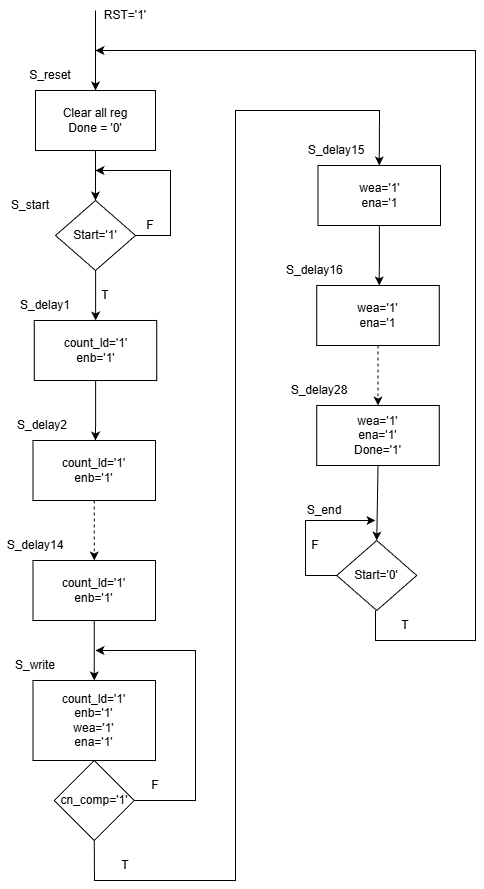
\includegraphics[width=0.5\textwidth]{Image/Sigmoid_controller.png}
    \label{fig:Sigmoid_FSM}
\end{figure}
\begin{itemize}
    \item FSM gồm 31 trạng thái nhưng cấu trúc rất đơn giản, chia
    thành 3 giai đoạn:

    \item \textbf{Nạp pipeline} (\texttt{S\_delay1..S\_delay14}):
    14 chu kỳ liên tục đọc dữ liệu từ BRAM và đẩy vào pipeline.
    \texttt{count\_ld} và \texttt{enb} đều bật. Kết quả đầu tiên
    chưa sẵn sàng ở đầu ra.

    \item \textbf{Ghi kết quả} (\texttt{S\_write}): từ chu kỳ thứ 15,
    kết quả sigmoid bắt đầu xuất hiện ở \texttt{dina}. FSM bật thêm
    \texttt{ena} và \texttt{wea} để ghi ra BRAM đầu ra, đồng thời
    tiếp tục đọc dữ liệu mới. Trạng thái này lặp cho đến khi
    \texttt{cn\_comp = '1'} — tức bộ đếm đã duyệt hết $C \times N$
    phần tử.

    \item \textbf{Xả pipeline} (\texttt{S\_delay15..S\_delay28}):
    14 chu kỳ tiếp tục ghi các kết quả còn nằm trong pipeline ra BRAM
    (\texttt{ena}, \texttt{wea} vẫn bật), không đọc thêm dữ liệu mới.
    Tại \texttt{S\_delay28}, bật \texttt{Done\_o = '1'}.

    \item \texttt{S\_end}: chờ \texttt{Start\_i} hạ rồi quay về
    \texttt{S\_reset}.
\end{itemize}

Nhờ kiến trúc pipeline, Sigmoid đạt throughput 1 phần tử/chu kỳ
trong giai đoạn \texttt{S\_write}. Tổng thời gian xử lý $C \times N$
phần tử là $C \times N + 28$ chu kỳ (gồm 14 chu kỳ nạp và 14 chu kỳ
xả pipeline).

\subsection{Softmax}
Softmax chuẩn hóa vector $[1, C]$ (đầu ra của AvgPool) thành phân phối
xác suất:
\begin{equation}
    y[i] = \frac{e^{x[i] - x_{\max}}}{\displaystyle\sum_{j=0}^{C-1}
    e^{x[j] - x_{\max}}}, \qquad i = 0, \ldots, C{-}1
\end{equation}
trong đó $x_{\max} = \max_j x[j]$ được cung cấp từ bên ngoài, dùng để
dịch đầu vào về miền không dương trước khi tính exp nhằm tránh tràn
số.

Tại giai đoạn 3: $C = 16$. Khác với Sigmoid xử lý bản đồ đặc trưng 2D lớn,
Softmax chỉ làm việc trên vector 1 chiều 16 phần tử nhưng cần
\textbf{hai lượt duyệt}: lượt 1 tính tổng $\sum e^{x_i - x_{\max}}$,
lượt 2 chia từng $e^{x_i - x_{\max}}$ cho tổng đó.

Mã giả:
\begin{Verbatim}[frame=single]
Input:
    input[C]
    X_max
    C

Output:
    output[C]

X_add = 0

For C_c = 0 to C - 1:

    addrb = C_c
    doutb = input[addrb]

    X_sub = doutb - X_max
    Exp_out = exp(X_sub)

    X_add = X_add + Exp_out


For C_c = 0 to C - 1:

    addrb = C_c
    doutb = input[addrb]

    X_sub = doutb - X_max
    Exp_out = exp(X_sub)

    Div_out = Exp_out / X_add

    dina = Div_out
    addra = C_c

    output[addra] = dina

Return output
\end{Verbatim}

\begin{enumerate}
    \item \textbf{Datapath}
\end{enumerate}
\begin{figure}[h]{Datapath của Softmax}
    \centering
    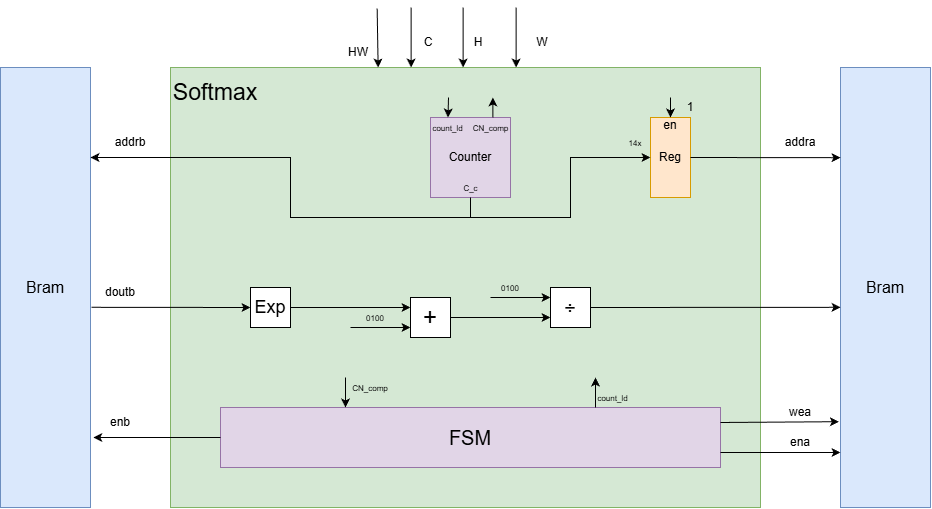
\includegraphics[width=\textwidth]{Image/Softmax_datapath.png}
    \label{fig:Softmax_datapath}
\end{figure}
\begin{itemize}
    \item Tín hiệu kết thúc: \texttt{C\_comp}.

    \item \textbf{Địa chỉ đọc}: $\texttt{addrb} = \texttt{C\_c}$ — truy cập
    trực tiếp vì đầu vào là vector 1 chiều.

    \item \textbf{Phép trừ}: tính $\texttt{doutb} - x_{\max}$, đưa
    mọi giá trị về $\leq 0$.

    \item \textbf{Bộ exp}: \texttt{exp\_softmax} là phiên bản đơn giản
    hóa của \texttt{exp\_continuos} — chỉ dùng LUT dương
    (\texttt{exp\_lut\_int/frac/frac2}) vì đầu vào sau khi lấy đối
    luôn $\geq 0$. Cấu trúc pipeline 4 chu kỳ tương tự:
    1 thanh ghi đầu vào + 1 thanh ghi LUT + 2 thanh ghi nhân
    Booth--Wallace.

    \item \textbf{Tích lũy tổng}: cộng dồn $e^{x_i - x_{\max}}$
    qua $C$ phần tử ở lượt 1. MUX 2:1 reset thanh ghi tích lũy về 0
    đầu lượt 1. Sau khi cộng xong, tổng
    $\sum e^{x_j - x_{\max}}$ được giữ cố định cho lượt 2.

    \item \textbf{Bộ chia}: \texttt{Div\_16bit\_continuos} chia
    $e^{x_i - x_{\max}}$ cho tổng ở lượt 2, pipeline 8 chu kỳ
    (Goldschmidt 3 vòng lặp). Tổng trễ pipeline từ \texttt{addrb} đến
    \texttt{dina}: $2\ (\text{BRAM}) + 4\ (\text{Exp}) +
    8\ (\text{Div}) = 14$ chu kỳ.

    \item \textbf{Địa chỉ ghi}: \texttt{addra} đi qua chuỗi
    \textbf{14 thanh ghi} pipeline (ký hiệu ``14x'' trên sơ đồ), chỉ
    sử dụng ở lượt 2.
\end{itemize}

\begin{enumerate}
    \setcounter{enumi}{1}
    \item \textbf{FSM}
\end{enumerate}
\begin{figure}[h]{FSM của Softmax}
    \centering
    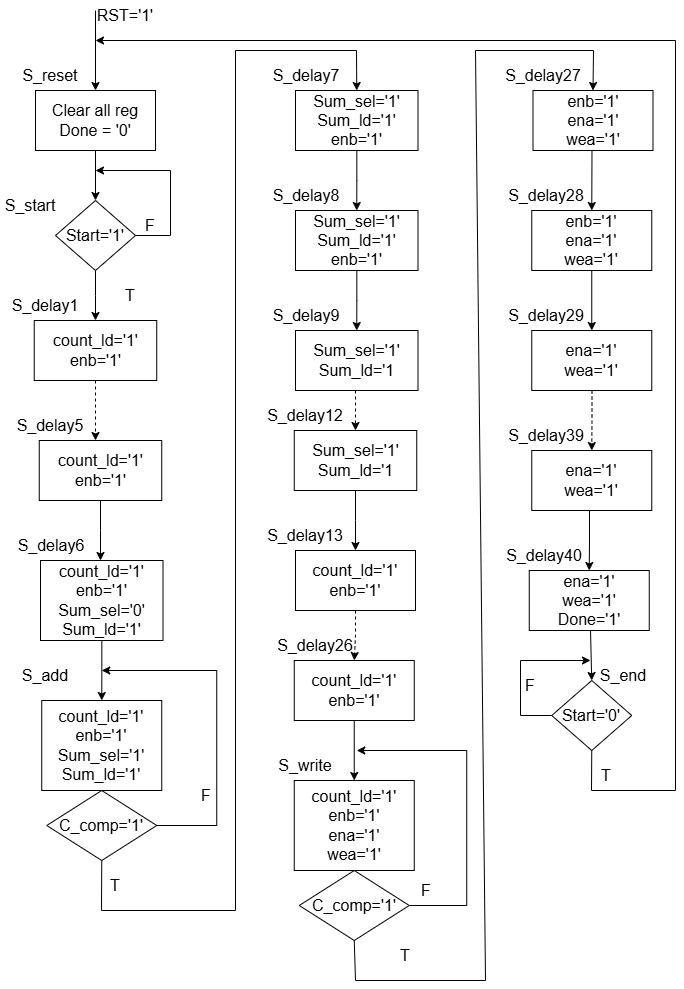
\includegraphics[width=0.65\textwidth]{Image/Softmax_controller.png}
    \label{fig:Softmax_FSM}
\end{figure}
\begin{itemize}
    \item FSM gồm 45 trạng thái, chia thành 4 giai đoạn:

    \item \textbf{Giai đoạn 1 — Nạp pipeline exp}
    (\texttt{S\_delay1..S\_delay6}): 6 chu kỳ đọc dữ liệu từ BRAM
    và đẩy vào pipeline exp (2 chu kỳ BRAM + 4 chu kỳ exp).
    \texttt{S\_delay6} reset \texttt{Sum} về 0
    (\texttt{Sum\_sel = '0'}).

    \item \textbf{Giai đoạn 2 — Tích lũy tổng exp}
    (\texttt{S\_add}): cộng dồn $e^{x_i - x_{\max}}$ vào \texttt{Sum},
    lặp đến khi \texttt{C\_comp = '1'} (hết $C$ phần tử).
    \texttt{S\_delay7..S\_delay12} (6 chu kỳ) xả pipeline exp — các
    giá trị còn trong pipeline tiếp tục được cộng vào \texttt{Sum}.
    Sau giai đoạn này, \texttt{Sum} chứa tổng đầy đủ.

    \item \textbf{Giai đoạn 3 — Nạp pipeline chia}
    (\texttt{S\_delay13..S\_delay26}): 14 chu kỳ khởi động lượt duyệt
    thứ hai. Bộ đếm \texttt{C\_c} chạy lại từ 0, dữ liệu đọc lại từ BRAM,
    tính lại $e^{x_i - x_{\max}}$ rồi đẩy vào bộ chia (chia cho
    \texttt{Sum} cố định).

    \item \textbf{Giai đoạn 4 — Ghi kết quả}
    (\texttt{S\_write}): bật \texttt{ena}, \texttt{wea}, ghi kết quả
    softmax ra BRAM đầu ra, lặp đến khi \texttt{C\_comp = '1'}.
    \texttt{S\_delay27..S\_delay40} (14 chu kỳ) xả pipeline chia,
    tiếp tục ghi các kết quả còn lại. Tại \texttt{S\_delay40}, bật
    \texttt{Done\_o = '1'}.

    \item \texttt{S\_end}: chờ \texttt{Start\_i} hạ rồi quay về
    \texttt{S\_reset}.
\end{itemize}

Do cần hai lượt duyệt (tính tổng rồi chia), Softmax có số trạng thái
FSM lớn nhất trong các mô-đun kích hoạt dù chỉ xử lý $C = 16$ phần
tử. Tổng thời gian: $C + 6 + 6$ (lượt 1) $+ 14 + C + 14$ (lượt 2)
$= 2C + 40$ chu kỳ.

\section{Tính toán chú ý}
\subsection{Element-wise Multiply}
Element-wise Multiply (ElemMul) thực hiện phép nhân phần tử giữa bản đồ đặc trưng
đầu vào $\text{input}[C, H, W]$ với hai bản đồ chú ý sau sigmoid:
$\text{sig\_h}[C, H, 1]$ và $\text{sig\_w}[C, 1, W]$:
\begin{equation}
    x_1[c][h][w] = \text{input}[c][h][w] \times
    \text{sig\_h}[c][h] \times \text{sig\_w}[c][w]
\end{equation}

Mô-đun đọc đồng thời từ \textbf{3 BRAM}: BRAM1 chứa $\text{sig\_h}$
(kích thước $C \times H$), BRAM2 chứa $\text{sig\_w}$
(kích thước $C \times W$), BRAM3 chứa $\text{input}$
(kích thước $C \times H \times W$). Kết quả ghi vào BRAM đầu ra.

Tại giai đoạn 3: $C = 16$, $H = W = 16$, tổng $C \times HW = 4096$
phần tử.

Mã giả:
\begin{Verbatim}[frame=single]
Input:
    sig_h[C * H]
    sig_w[C * W]
    input[C * H * W]
    C, H, W

Output:
    output[C * H * W]

HW = H * W

For C_c = 0 to C - 1:
    For H_c = 0 to H - 1:
        For W_c = 0 to W - 1:

            addrb1 = C_c * H + H_c
            doutb1 = sig_h[addrb1]

            addrb2 = C_c * W + W_c
            doutb2 = sig_w[addrb2]

            addrb3 = C_c * HW + H_c * W + W_c
            doutb3 = input[addrb3]

            Mul_out1 = doutb1 * doutb2
            Mul_out2 = Mul_out1 * doutb3

            dina = Mul_out2

            addra = C_c * HW + H_c * W + W_c
            output[addra] = dina

Return output
\end{Verbatim}

\begin{enumerate}
    \item \textbf{Datapath}
\end{enumerate}

\begin{itemize}
    \item Tín hiệu kết thúc:
    \texttt{CHW\_comp = W\_comp AND H\_comp AND C\_comp}.

    \item \textbf{Địa chỉ đọc}: ba BRAM có cách đánh địa chỉ khác
    nhau do kích thước khác nhau:
    \begin{itemize}
        \item $\texttt{addrb1} = \texttt{C\_c} \times H + \texttt{H\_c}$ — đọc
        $\text{sig\_h}[c][h]$
        \item $\texttt{addrb2} = \texttt{C\_c} \times W + \texttt{W\_c}$ — đọc
        $\text{sig\_w}[c][w]$
        \item $\texttt{addrb3} = \texttt{C\_c} \times HW + \texttt{H\_c} \times W + \texttt{W\_c}$
        — đọc $\text{input}[c][h][w]$
    \end{itemize}

    \item \textbf{Pipeline nhân 2 tầng}: phép nhân 3 toán hạng được
    tách thành 2 phép nhân Booth--Wallace nối tiếp:
    \begin{itemize}
        \item Tầng 1: $\texttt{doutb1} \times \texttt{doutb2}$
        (sig\_h $\times$ sig\_w), chốt qua thanh ghi
        \item Tầng 2: kết quả tầng 1 nhân với \texttt{doutb3}
        (đã qua 1 thanh ghi trễ để đồng bộ)
    \end{itemize}
    Tổng trễ pipeline: $2\ (\text{BRAM}) + 2\ (\text{2 tầng nhân})
    = 4$ chu kỳ.

    \item \textbf{Địa chỉ ghi}: \texttt{addra} đi qua \textbf{4 thanh
    ghi} pipeline (ký hiệu ``4x'' trên sơ đồ) để đồng bộ với trễ
    tính toán.
\end{itemize}

\begin{figure}[h]{Datapath của ElemMul}
    \centering
    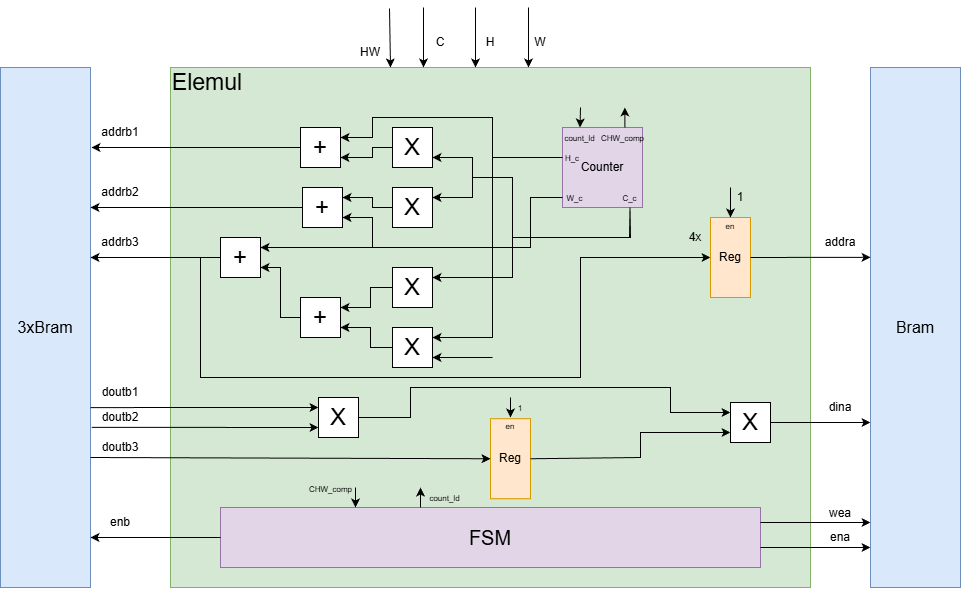
\includegraphics[width=\textwidth]{Image/Elemul_datapath.png}
    \label{fig:Elemul_datapath}
\end{figure}

\begin{enumerate}
    \setcounter{enumi}{1}
    \item \textbf{FSM}
\end{enumerate}
\begin{figure}[h]{FSM của ElemMul}
    \centering
    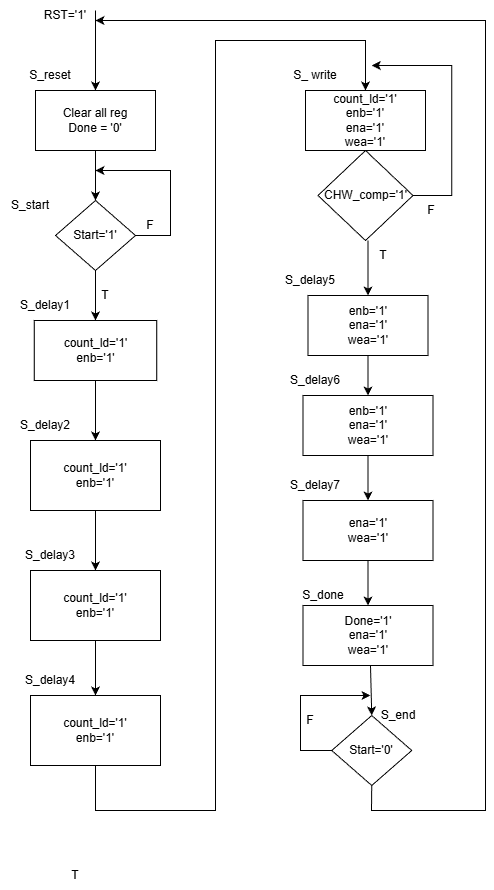
\includegraphics[width=0.55\textwidth]{Image/Elemul_controller.png}
    \label{fig:Elemul_FSM}
\end{figure}
\begin{itemize}
    \item FSM gồm 12 trạng thái, cấu trúc đơn giản tương tự Sigmoid:

    \item \textbf{Nạp pipeline} (\texttt{S\_delay1..S\_delay4}):
    4 chu kỳ đọc dữ liệu từ 3 BRAM và đẩy qua 2 tầng nhân.
    \texttt{count\_ld} và \texttt{enb} đều bật.

    \item \textbf{Ghi kết quả} (\texttt{S\_write}): bật thêm
    \texttt{ena}, \texttt{wea}; mỗi chu kỳ ghi một kết quả, đồng thời
    tiếp tục đọc và nhân phần tử tiếp theo. Lặp đến khi
    \texttt{CHW\_comp = '1'}.

    \item \textbf{Xả pipeline} (\texttt{S\_delay5..S\_delay7}):
    3 chu kỳ ghi nốt kết quả còn trong pipeline (\texttt{ena},
    \texttt{wea} vẫn bật). \texttt{S\_delay5}, \texttt{S\_delay6} vẫn
    bật \texttt{enb} để đẩy dữ liệu cuối qua bộ nhân.

    \item \texttt{S\_done}, \texttt{S\_end}: bật \texttt{Done\_o = '1'},
    \texttt{ena} và \texttt{wea} vẫn bật tại \texttt{S\_done} để ghi
    phần tử cuối cùng. Chờ \texttt{Start\_i} hạ rồi quay về
    \texttt{S\_reset}.
\end{itemize}

ElemMul là mô-đun đơn giản nhất trong nhóm tính toán chú ý: không
có bộ tích lũy hay bộ chia, chỉ gồm 2 bộ nhân pipeline. Throughput
đạt 1 phần tử/chu kỳ, tổng thời gian $C \times HW + 7$ chu kỳ.

\subsection{Matmul}
Matmul thực hiện phép nhân ma trận giữa vector softmax $[1, C]$ và
bản đồ đặc trưng đã reshape $[C, HW]$, cho ra kết quả $[1, HW]$:
\begin{equation}
    \text{out}[n] = \sum_{c=0}^{C-1}
    \text{softmax}[c] \times \text{feature}[c][n],
    \qquad n = 0, \ldots, HW{-}1
\end{equation}

Trong luồng EMA, phép matmul được gọi hai lần (cho cặp x11$\times$x12
và x21$\times$x22), mỗi lần là một instance riêng của mô-đun này.

Tại giai đoạn 3: $C = 16$, $HW = 256$. BRAM1 chứa vector softmax
$[1, C]$, BRAM2 chứa bản đồ đặc trưng $[C, HW]$.

Mã giả:
\begin{Verbatim}[frame=single]
Input:
    softmax[C]
    feature[C * H * W]
    C, H, W

Output:
    output[H * W]

HW = H * W

For HW_c = 0 to HW - 1:

    X_add = 0

    For C_c = 0 to C - 1:

        addrb1 = C_c
        doutb1 = softmax[addrb1]

        addrb2 = C_c * HW + HW_c
        doutb2 = feature[addrb2]

        Mul_out = doutb1 * doutb2

        X_add = X_add + Mul_out

    dina = X_add
    addra = HW_c

    output[addra] = dina

Return output
\end{Verbatim}

\begin{enumerate}
    \item \textbf{Datapath}
\end{enumerate}
\begin{figure}[h]{Datapath của Matmul}
    \centering
    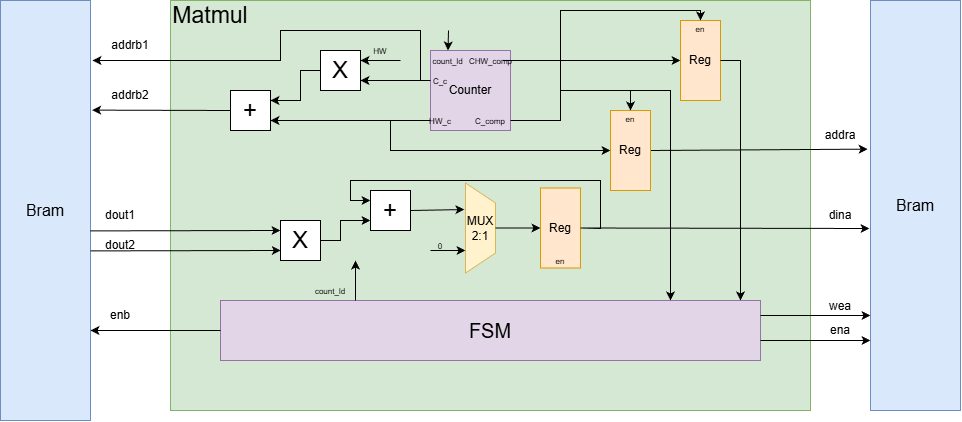
\includegraphics[width=\textwidth]{Image/Matmul_datapath.png}
    \label{fig:Matmul_datapath}
\end{figure}
\begin{itemize}
    \item Tín hiệu kết thúc:
    \texttt{CHW\_comp = C\_comp AND HW\_comp}.

    \item \textbf{Địa chỉ đọc}: hai BRAM có cách đánh địa chỉ khác
    nhau:
    \begin{itemize}
        \item $\texttt{addrb1} = \texttt{C\_c}$ — đọc $\text{softmax}[c]$
        (vector 1 chiều)
        \item $\texttt{addrb2} = \texttt{C\_c} \times HW + \texttt{HW\_c}$ — đọc
        $\text{feature}[c][n]$ (ma trận 2 chiều)
    \end{itemize}

    \item \textbf{MAC}: bộ nhân Booth--Wallace tính
    $\texttt{doutb1} \times \texttt{doutb2}$, kết quả qua thanh ghi
    rồi cộng tích lũy vào bộ tích lũy 16-bit. MUX 2:1 reset
    bộ tích lũy về 0 đầu mỗi điểm đầu ra mới.

    \item \textbf{Kết quả}: giá trị bộ tích lũy ghi trực tiếp ra
    \texttt{dina} của BRAM đầu ra (không cần dịch bit vì bộ nhân
    Booth--Wallace đã trả về kết quả Q8.8).

    \item \textbf{Địa chỉ ghi}: \texttt{addra} chốt từ \texttt{HW\_c}
    qua thanh ghi khi \texttt{C\_comp = '1'} (kết thúc tích lũy một điểm).
\end{itemize}

\newpage

\begin{enumerate}
    \setcounter{enumi}{1}
    \item \textbf{FSM}
\end{enumerate}
\begin{figure}[h]{FSM của Matmul}
    \centering
    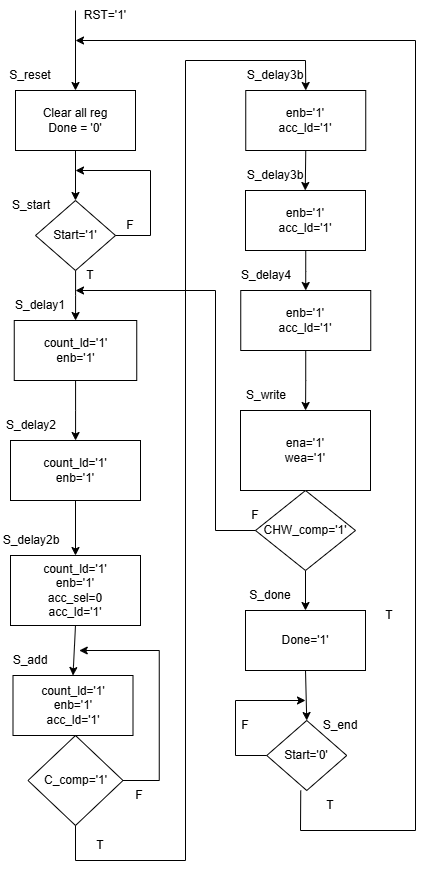
\includegraphics[width=0.5\textwidth]{Image/Matmul_controller.png}
    \label{fig:Matmul_FSM}
\end{figure}
\begin{itemize}
    \item FSM gồm 12 trạng thái, cấu trúc tương tự Conv1x1:

    \item \texttt{S\_delay1}, \texttt{S\_delay2}: 2 chu kỳ chờ BRAM
    trả dữ liệu.

    \item \texttt{S\_delay2b}: xóa bộ tích lũy về 0
    (\texttt{acc\_sel = '0'}), đồng thời chốt tích đầu tiên từ bộ
    nhân.

    \item \texttt{S\_add}: cộng dồn $\text{softmax}[c] \times
    \text{feature}[c][n]$ vào bộ tích lũy, lặp đến khi
    \texttt{C\_comp = '1'} (hết $C$ kênh).

    \item \texttt{S\_delay3b}, \texttt{S\_delay3}, \texttt{S\_delay4}:
    3 chu kỳ xả pipeline — chốt các tích còn trong thanh ghi bộ nhân
    vào bộ tích lũy.

    \item \texttt{S\_write}: bật \texttt{ena}, \texttt{wea}, ghi
    \texttt{acc} ra BRAM đầu ra. Kiểm tra \texttt{CHW\_comp}: nếu
    chưa xong quay về \texttt{S\_delay1} tính điểm tiếp; nếu xong
    chuyển sang \texttt{S\_done}.

    \item \texttt{S\_done}, \texttt{S\_end}: bật \texttt{Done\_o = '1'},
    chờ \texttt{Start\_i} hạ.
\end{itemize}

Matmul có cấu trúc FSM giống Conv1x1 (tích lũy MAC rồi ghi), nhưng
đơn giản hơn vì không cần bias. Tổng thời gian:
$HW \times (C + 6) + 1$ chu kỳ (mỗi điểm đầu ra cần $C$ chu kỳ
tích lũy + 6 chu kỳ pipeline/ghi).

\subsection{AddSigmoid}
AddSigmoid cộng hai kết quả matmul rồi áp sigmoid lên tổng, tạo ra
tensor trọng số chú ý $[1, H, W]$:
\begin{equation}
    \text{weights}[n] = \sigma\bigl(\text{matmul\_1}[n]
    + \text{matmul\_2}[n]\bigr)
    = \frac{1}{1 + e^{-(\text{doutb1}[n]\,+\,\text{doutb2}[n])}}
\end{equation}
trong đó $n = 0, \ldots, HW{-}1$ (mỗi phần tử tương ứng một vị trí
không gian).

Mô-đun có cấu trúc gần giống Sigmoid (mục \ref{fig:Sigmoid_datapath}),
chỉ khác ở đầu vào: thay vì đọc từ 1 BRAM, AddSigmoid đọc đồng thời
từ \textbf{2 BRAM} (hai kết quả matmul) với cùng địa chỉ, cộng chúng
lại trước khi đẩy vào pipeline sigmoid.

Tại giai đoạn 3: $H = W = 16$, $HW = 256$ phần tử.

Mã giả:
\begin{Verbatim}[frame=single]
Input:
    input1[H * W]
    input2[H * W]
    H, W

Output:
    output[H * W]

HW = H * W

For HW_c = 0 to HW - 1:

    addrb1 = HW_c
    doutb1 = input1[addrb1]

    addrb2 = HW_c
    doutb2 = input2[addrb2]

    X_add = doutb1 + doutb2

    Exp_out = exp(-X_add)

    Div_in = 1 + Exp_out
    Div_out = 1 / Div_in

    dina = Div_out
    addra = HW_c

    output[addra] = dina

Return output
\end{Verbatim}

\begin{enumerate}
    \item \textbf{Datapath}
\end{enumerate}
\begin{figure}[h]{Datapath của AddSigmoid}
    \centering
    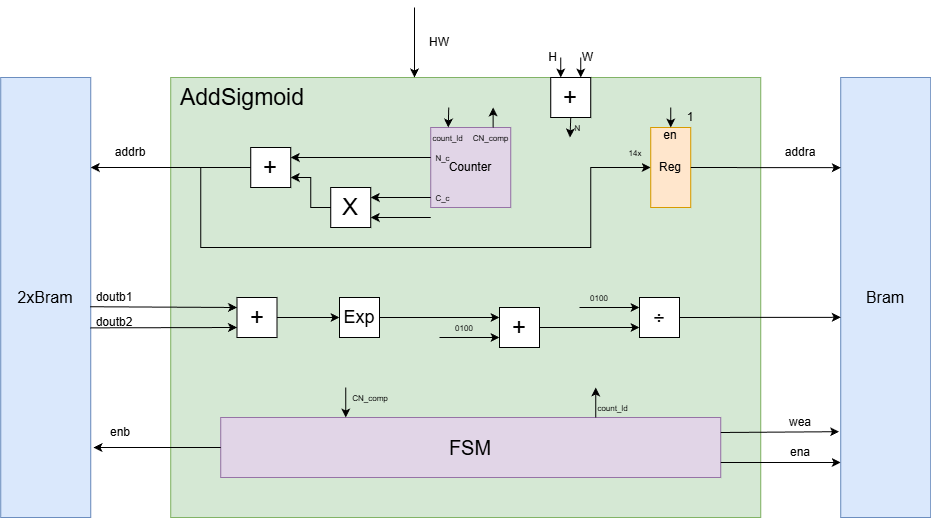
\includegraphics[width=\textwidth]{Image/AddSigmoid_datapath.png}
    \label{fig:AddSigmoid_datapath}
\end{figure}
\begin{itemize}
    \item Tín hiệu kết thúc: \texttt{HW\_comp}. Địa chỉ đọc
    $\texttt{addrb} = \texttt{HW\_c}$, dùng chung cho cả hai BRAM.

    \item \textbf{Bộ cộng đầu vào}: cộng tổ hợp
    $\texttt{doutb1} + \texttt{doutb2}$, không thêm trễ pipeline.
    Đây là điểm khác biệt duy nhất so với Sigmoid.

    \item \textbf{Pipeline sigmoid}: giống hệt Sigmoid — kết quả cộng
    đi vào \texttt{exp\_continuos} (4 chu kỳ), cộng \texttt{0x0100},
    rồi chia bởi \texttt{Div\_16bit\_continuos} (8 chu kỳ). Tổng trễ
    pipeline: $2\ (\text{BRAM}) + 4\ (\text{Exp}) + 8\ (\text{Div})
    = 14$ chu kỳ.

    \item \textbf{Địa chỉ ghi}: \texttt{addra} đi qua \textbf{14 thanh
    ghi} pipeline (ký hiệu ``14x'') để đồng bộ với trễ tính toán.
\end{itemize}

\begin{enumerate}
    \setcounter{enumi}{1}
    \item \textbf{FSM}
\end{enumerate}

FSM của AddSigmoid có cấu trúc \textbf{giống hệt} Sigmoid
(Hình~\ref{fig:Sigmoid_FSM}), gồm 31 trạng thái chia thành 3 giai
đoạn:
\begin{itemize}
    \item \textbf{Nạp pipeline} (\texttt{S\_delay1..S\_delay14}):
    14 chu kỳ đọc đồng thời từ 2 BRAM, cộng và đẩy vào pipeline.

    \item \textbf{Ghi kết quả} (\texttt{S\_write}): mỗi chu kỳ ghi
    một giá trị sigmoid ra BRAM đầu ra, lặp đến khi
    \texttt{HW\_comp = '1'}.

    \item \textbf{Xả pipeline} (\texttt{S\_delay15..S\_delay28}):
    14 chu kỳ ghi nốt kết quả còn trong pipeline. Tại
    \texttt{S\_delay28}, bật \texttt{Done\_o = '1'}.
\end{itemize}

Tổng thời gian: $HW + 28$ chu kỳ, throughput 1 phần tử/chu kỳ — giống
Sigmoid nhưng xử lý ít phần tử hơn ($HW = 256$ thay vì
$C \times HW = 4096$).

\subsection{FinalMul}
FinalMul là bước cuối cùng của mô-đun EMA, nhân từng phần tử bản đồ đặc trưng
đầu vào $\text{input}[C, H, W]$ với trọng số chú ý đã qua
sigmoid $\text{weights}[1, H, W]$ (broadcast theo chiều kênh):
\begin{equation}
    \text{output}[c][h][w] = \text{input}[c][h][w]
    \times \text{weights}[h][w]
\end{equation}

Mô-đun đọc đồng thời từ \textbf{2 BRAM}: BRAM1 chứa
$\text{weights}[1, HW]$ (256 phần tử), BRAM2 chứa
$\text{input}[C, HW]$ (4096 phần tử). Kết quả ghi vào BRAM đầu ra.

Tại giai đoạn 3: $C = 16$, $H = W = 16$, tổng $C \times HW = 4096$
phần tử.

Mã giả:
\begin{Verbatim}[frame=single]
Input:
    weights[H * W]
    input[C * H * W]
    C, H, W

Output:
    output[C * H * W]

HW = H * W

For C_c = 0 to C - 1:
    For HW_c = 0 to HW - 1:

        addrb1 = HW_c
        doutb1 = weights[addrb1]

        addrb2 = C_c * HW + HW_c
        doutb2 = input[addrb2]

        Mul_out = doutb1 * doutb2

        dina = Mul_out
        addra = C_c * HW + HW_c

        output[addra] = dina

Return output
\end{Verbatim}

\begin{enumerate}
    \item \textbf{Datapath}
\end{enumerate}
\begin{figure}[h]{Datapath của FinalMul}
    \centering
    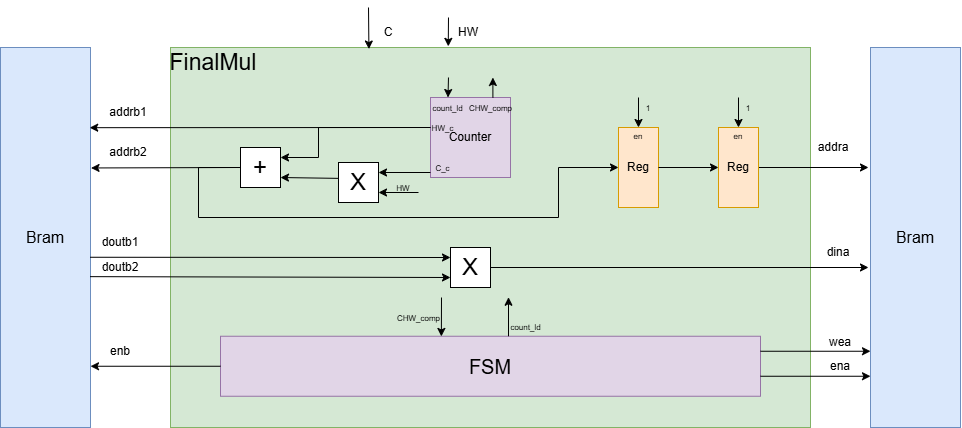
\includegraphics[width=\textwidth]{Image/FinalMul_datapath.png}
    \label{fig:FinalMul_datapath}
\end{figure}
\begin{itemize}
    \item Tín hiệu kết thúc:
    \texttt{CHW\_comp = HW\_comp AND C\_comp}.

    \item \textbf{Địa chỉ đọc}:
    \begin{itemize}
        \item $\texttt{addrb1} = HW\_c$ — đọc
        $\text{weights}[hw]$ (vector 1 chiều, lặp lại mỗi kênh)
        \item $\texttt{addrb2} = C\_c \times HW + HW\_c$ — đọc
        $\text{input}[c][hw]$
    \end{itemize}

    \item \textbf{Bộ nhân}: một bộ nhân Booth--Wallace duy nhất tính
    $\texttt{doutb1} \times \texttt{doutb2}$, kết quả Q8.8 chốt qua
    1 thanh ghi ra \texttt{dina}. Không cần bộ tích lũy vì mỗi phần
    tử đầu ra chỉ là một phép nhân đơn.

    \item \textbf{Địa chỉ ghi}: \texttt{addra} đi qua \textbf{2 thanh
    ghi} pipeline (tương ứng 2 chu kỳ BRAM + 1 chu kỳ nhân = 3 chu kỳ
    trễ tổng, trong đó 1 chu kỳ tính địa chỉ song song với BRAM).
\end{itemize}

\begin{enumerate}
    \setcounter{enumi}{1}
    \item \textbf{FSM}
\end{enumerate}
\begin{figure}[h]{FSM của FinalMul}
    \centering
    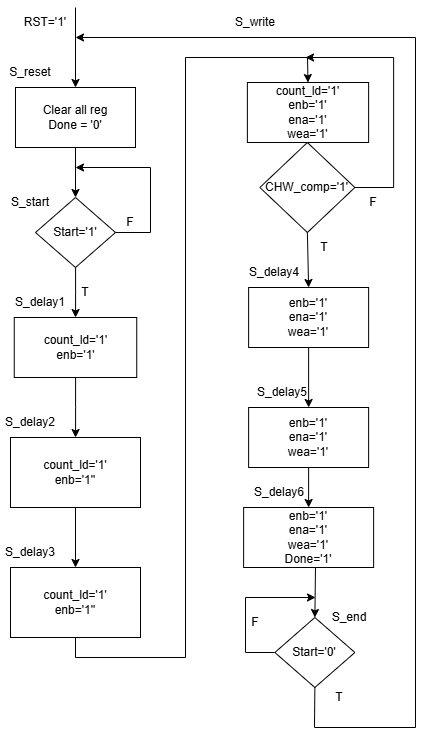
\includegraphics[width=0.55\textwidth]{Image/FinalMul_controller.png}
    \label{fig:FinalMul_FSM}
\end{figure}
\begin{itemize}
    \item FSM chỉ gồm 10 trạng thái — đơn giản nhất trong toàn bộ
    thiết kế:

    \item \textbf{Nạp pipeline} (\texttt{S\_delay1..S\_delay2}):
    2 chu kỳ chờ BRAM trả dữ liệu. \texttt{S\_delay3} thêm 1 chu kỳ
    cho bộ nhân chốt kết quả đầu tiên.

    \item \textbf{Ghi kết quả} (\texttt{S\_write}): bật \texttt{ena},
    \texttt{wea}; mỗi chu kỳ đọc--nhân--ghi một phần tử. Lặp đến khi
    \texttt{CHW\_comp = '1'}.

    \item \textbf{Xả pipeline} (\texttt{S\_delay3..S\_delay4}):
    2 chu kỳ ghi nốt các phần tử cuối còn trong pipeline.
    \texttt{S\_delay5} (\texttt{S\_delay6} trong code) ghi phần tử
    cuối cùng, bật \texttt{Done\_o = '1'}.

    \item \texttt{S\_end}: chờ \texttt{Start\_i} hạ rồi quay về
    \texttt{S\_reset}.
\end{itemize}

FinalMul có cấu trúc đơn giản nhất vì chỉ cần 1 phép nhân trên mỗi
phần tử, không tích lũy, không chia, không hàm kích hoạt. Throughput
đạt 1 phần tử/chu kỳ, tổng thời gian $C \times HW + 6$ chu kỳ.

\chapter{MÔ PHỎNG VÀ ĐÁNH GIÁ}
\section{Môi trường mô phỏng}

Toàn bộ quá trình mô phỏng chức năng được thực hiện trong
Xilinx Vivado 2018.3, sử dụng bộ mô phỏng tích hợp XSIM. Thiết bị được chọn
là FPGA Artix-7 XC7A200T-2FBG676C trên bo mạch AC701, tần số clock hệ thống
100\,MHz (chu kỳ 10\,ns).

Mô-đun EMA top-level được kiểm tra trọn vẹn như một hộp đen. Để giảm thời gian
mô phỏng và độ phức tạp của testbench, toàn bộ dữ liệu đầu vào -- bao gồm
bản đồ đặc trưng, weight, bias và tham số GroupNorm -- được nạp sẵn trong BRAM ROM
thông qua giá trị khởi tạo trong mã VHDL, bỏ qua bước ghi dữ liệu qua cổng
ngoài. Testbench chỉ cần kích hoạt tín hiệu \texttt{Start}, chờ tín hiệu
\texttt{Done} rồi đọc toàn bộ output qua BRAM Port~B.

Dữ liệu tham chiếu được khởi tạo từ mô hình PyTorch (ResNet50 + EMA, tệp trọng số \texttt{ema\_model\_best.pth}) với cùng cấu hình bộ trọng số đã được lượng tử hóa sang định dạng dấu phẩy tĩnh Q8.8. Giá trị đầu ra kỳ vọng của mô-đun EMA thuộc nhóm~0 (group~0) của khối đầu tiên trong giai đoạn 3 (Stage 3, tương ứng với tên gọi \texttt{layer2.0} trong mã nguồn PyTorch) được trích xuất ra tệp \texttt{q8\_8\_ema\_output.coe} dưới dạng 4096 số hex 16-bit (tương đương cấu trúc tensor $16 \times 16 \times 16$). Sai lệch giữa kết quả thực thi phần cứng và mô hình tham chiếu được đánh giá thông qua hiệu tuyệt đối tính theo đơn vị LSB (Least Significant Bit, tương ứng với giá trị $1/256 \approx 0{,}004$ trong định dạng Q8.8).
\begin{itemize}
    \item \textbf{Tạo dữ liệu tham chiếu:} Chạy mô hình PyTorch (ResNet50 + EMA, tệp trọng số \texttt{ema\_model\_best.pth}) với đầu vào dữ liệu CIFAR-100 đã được lượng tử hóa sang định dạng Q8.8. Giá trị đầu ra của mô-đun EMA thuộc nhóm~0 (group~0) của khối đầu tiên trong giai đoạn 3 (Stage 3, tương ứng với tên gọi \texttt{layer2.0} trong mã nguồn PyTorch) được trích xuất ra tệp định dạng \texttt{.coe} dưới dạng 4096 số nguyên 16-bit có dấu (tương đương cấu trúc tensor $16 \times 16 \times 16$).

    \item \textbf{Nạp dữ liệu vào testbench:} Tệp
    \texttt{fmap\_q8p8\_16bit\_4096.coe} được dùng làm input bản đồ đặc trưng. Các tham số
    weight, bias của Conv3$\times$3, Conv1$\times$1 và GroupNorm được nhúng sẵn trong
    BRAM ROM, đồng nhất với bộ trọng số Python. Testbench ghi 4096 giá trị vào BRAM
    Port~A, sau đó phát xung \texttt{Start} và quan sát toàn bộ pipeline chạy tự động
    qua 14 trạng thái FSM.
\end{itemize}

Kết quả đầu ra từ BRAM Port~B được so sánh với tệp tham chiếu Python. Sai lệch
được đánh giá bằng hiệu tuyệt đối tính theo đơn vị LSB (Least Significant Bit,
tương ứng $1/256 \approx 0{,}004$ trong Q8.8).

\section{Thời gian xử lý các mô-đun}

\begin{figure}[h]{Dạng sóng thời gian chạy mô-đun EMA trong mô phỏng}
    \centering
    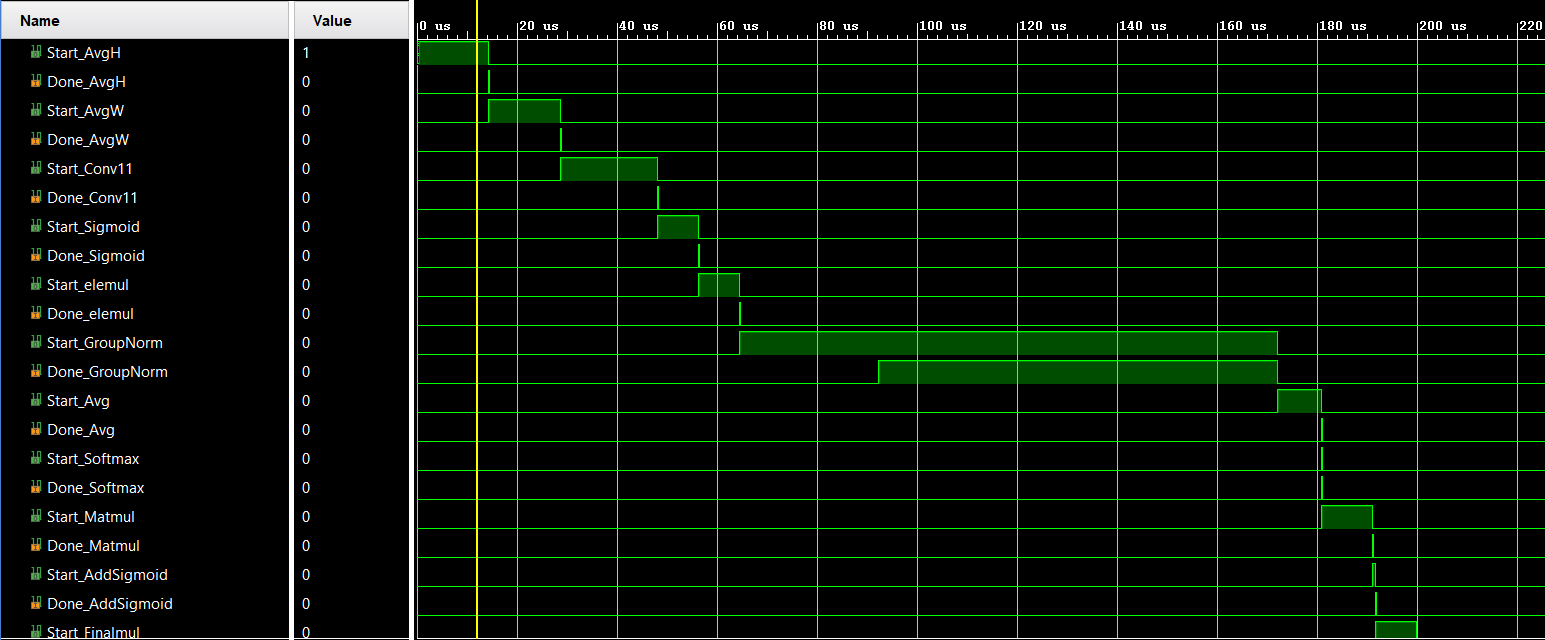
\includegraphics[width=\textwidth]{Image/Runtime.png}
    \label{fig:runtime}
\end{figure}

Mô phỏng sử dụng clock chu kỳ 2\,ns (tần số 500\,MHz) để rút ngắn thời gian mô
phỏng. Mỗi cạnh lên tương ứng một chu kỳ xử lý.

\begin{table}[h]{Thời gian xử lý từng khối trong mô-đun EMA}
    \centering
    \begin{tabular}{|l|r|r|r|}
        \hline
        \textbf{Mô-đun} & \textbf{Bắt đầu (ns)} & \textbf{Kết thúc (ns)}
            & \textbf{Số chu kỳ} \\
        \hline
        Conv3$\times$3   & 21      & 172{,}055  & 86{,}017 \\
        AvgPoolH         & 31      & 14{,}359   & 7{,}164  \\
        AvgPoolW          & 14{,}361  & 28{,}699   & 7{,}169  \\
        Conv1$\times$1   & 28{,}701  & 48{,}159   & 9{,}729  \\
        Sigmoid          & 48{,}161  & 56{,}381   & 4{,}110  \\
        ElemMul          & 56{,}383  & 64{,}583   & 4{,}100  \\
        GroupNorm        & 64{,}585  & 92{,}235   & 13{,}825 \\
        AvgPool          & 172{,}057 & 180{,}827  & 4{,}385  \\
        Softmax          & 180{,}829 & 180{,}933  & 52       \\
        Matmul           & 180{,}935 & 191{,}177  & 5{,}121  \\
        AddSigmoid       & 191{,}179 & 191{,}791  & 306      \\
        FinalMul         & 191{,}721 & 199{,}919  & 4{,}099  \\
        \hline
        \textbf{EMA tổng} & \textbf{21} & \textbf{199{,}921}
            & \textbf{99{,}950} \\
        \hline
    \end{tabular}
    \label{tab:runtime}
\end{table}

Nhờ thiết kế song song trong FSM top-level (Hình~\ref{fig:EMA_FSM}), Conv3$\times$3
chạy đồng thời với toàn bộ nhánh~1 (AvgPoolH $\to$ AvgPoolW $\to$ Conv1$\times$1
$\to$ Sigmoid $\to$ ElemMul $\to$ GroupNorm). Nhánh~1 hoàn thành sau 46{,}097 chu kỳ,
trong khi Conv3$\times$3 cần 86{,}017 chu kỳ --- do đó Conv3$\times$3 là nút thắt
cổ chai và FSM phải chờ tại trạng thái \texttt{S\_GroupNorm} thêm
39{,}920 chu kỳ trước khi chuyển sang giai đoạn AvgPool. Tương tự, hai instance
AvgPool, Softmax và Matmul chạy song song với nhau, giúp giảm gần một nửa thời gian
cho giai đoạn chú ý so với xử lý tuần tự.

\section{Đánh giá độ chính xác}

Testbench nạp bản đồ đặc trưng đầu vào \texttt{fmap\_q8p8\_16bit\_4096.coe} (4096 giá
trị Q8.8) qua BRAM Port~A, phát xung \texttt{Start} và chờ tín hiệu \texttt{Done}.
Sau khi mô-đun hoàn tất, toàn bộ 4096 giá trị đầu ra được đọc từ BRAM Port~B và
xuất ra tệp \texttt{ema\_output.txt} dưới dạng hex 16-bit thông qua lệnh
\texttt{hwrite} của thư viện \texttt{IEEE.STD\_LOGIC\_TEXTIO}.

Kết quả phần cứng được so sánh với tệp tham chiếu
\texttt{q8\_8\_ema\_output.coe} --- đầu ra của mô hình Python sử dụng cùng bộ
trọng số Q8.8 và cùng bản đồ đặc trưng đầu vào. Sai lệch được đo bằng hiệu tuyệt đối
tính theo đơn vị LSB ($1\,\text{LSB} = 1/256 \approx 0{,}004$).

\begin{table}[h]{Phân bố sai số giữa phần cứng và Python tham chiếu}
    \centering
    \begin{tabular}{|c|r|r|r|}
        \hline
        \textbf{Sai số (LSB)} & \textbf{Số điểm} & \textbf{Tỷ lệ}
            & \textbf{Tích lũy} \\
        \hline
        0           & 1{,}504 & 36{,}73\% & 36{,}73\% \\
        1           & 806     & 19{,}68\% & 56{,}41\% \\
        2           & 814     & 19{,}88\% & 76{,}29\% \\
        3           & 842     & 20{,}56\% & 96{,}85\% \\
        4--5        & 74      & 1{,}81\%  & 98{,}66\% \\
        6--8        & 51      & 1{,}25\%  & 99{,}90\% \\
        9--11       & 4       & 0{,}10\%  & 100\%     \\
        \hline
    \end{tabular}
    \label{tab:error_dist}
\end{table}
Trong đó:
\begin{itemize}
    \item \textbf{Sai số (LSB)}: độ lệch tuyệt đối giữa kết quả phần cứng và Python tham chiếu, tính theo đơn vị LSB (Least Significant Bit). Với định dạng Q8.8, 1 LSB tương ứng $1/256 \approx 0{,}0039$.
    \item \textbf{Số điểm}: số lượng điểm đầu ra (trong tổng 4096) có mức sai số tương ứng.
    \item \textbf{Tỷ lệ}: phần trăm số điểm ở mức sai số đó so với tổng số điểm.
    \item \textbf{Tích lũy}: tỷ lệ phần trăm cộng dồn, cho biết bao nhiêu phần trăm điểm có sai số nhỏ hơn hoặc bằng mức đó.
\end{itemize}
Kết quả cho thấy:
\begin{itemize}
    \item \textbf{76{,}29\%} giá trị đầu ra có sai số $\leq 2$\,LSB
    (tương ứng $\leq 0{,}008$ trong Q8.8).

    \item \textbf{96{,}85\%} giá trị có sai số $\leq 3$\,LSB. Sai lệch 3\,LSB
    chủ yếu đến từ hiệu ứng tích lũy qua nhiều tầng tính toán: mỗi phép dịch bit
    \texttt{>>8} sau nhân Q8.8 gây mất phần lẻ, sai số này cộng dồn qua
    chuỗi Conv3$\times$3 $\to$ GroupNorm $\to$ Softmax $\to$ Matmul $\to$ Sigmoid.

    \item Sai số tối đa là 11\,LSB ($\approx 0{,}043$), xuất hiện tại vị trí
    \texttt{[0][15][0]} (phần cứng: \texttt{0x0025}, Python: \texttt{0x001A}).
    Các điểm có sai số lớn ($\geq 6$\,LSB) tập trung ở
    cột \texttt{ow=0} của hàng cuối (\texttt{oh=15}), nơi hiệu ứng biên
    (zero-padding) kết hợp với sai số xấp xỉ LUT trong Sigmoid và Exp gây
    lệch lớn nhất.

    \item Sai số trung bình toàn bộ tensor:
    \begin{align*}
                &\frac{0 \times 1504 + 1 \times 806 + 2 \times 814
                       + 3 \times 842 + \frac{4+5}{2} \times 74
                       + \frac{6+7+8}{3} \times 51 + \frac{9+10+11}{3} \times 4}{4096} \\
                \approx\; & 1{,}389\,\text{LSB} \Leftrightarrow 0{,}005
    \end{align*}
    cho thấy thiết kế phần cứng tái tạo chính xác
    hành vi của mô-đun EMA phần mềm trong phạm vi sai số lượng tử hóa Q8.8
    chấp nhận được.
\end{itemize}
Cần lưu ý rằng mô-đun EMA thực hiện cơ chế chú ý --- đầu ra là tích của
bản đồ đặc trưng đầu vào với trọng số chú ý qua sigmoid, nên các giá trị output
có biên độ rất nhỏ (phần lớn nằm trong khoảng $0$--$0{,}012$ ở Q8.8). Trong
ngữ cảnh này, vai trò của trọng số chú ý là xác định \textit{thứ tự ưu tiên}
giữa các vị trí không gian, không yêu cầu chính xác tuyệt đối về giá trị. Sai
số trung bình 1{,}38\,LSB ($\approx 0{,}005$) không làm thay đổi thứ tự này,
do đó thiết kế phần cứng đáp ứng yêu cầu chức năng của mô-đun EMA.

\chapter{THỰC NGHIỆM VÀ ĐÁNH GIÁ}

\section{Kết quả tổng hợp}

Thiết kế được tổng hợp và implementation trên thiết bị FPGA Artix-7 XC7A200T-2FBG676C
bằng Vivado 2018.3.

\begin{figure}[h]{Báo cáo tài nguyên sau implementation}
    \centering
    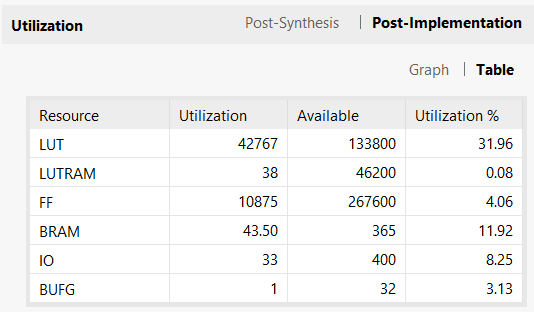
\includegraphics[width=0.6\textwidth]{Image/Resource.png}
    \label{fig:resource}
\end{figure}

Hình~\ref{fig:resource} cho thấy thiết kế sử dụng chủ yếu LUT (31{,}96\%) do
các phép nhân Booth-Wallace, adder tree và logic điều khiển FSM được ánh xạ hoàn
toàn bằng logic tổ hợp. BRAM chiếm 11{,}92\% để lưu
trữ bản đồ đặc trưng, weight, bias và các kết quả trung gian giữa các tầng. Số
flip-flop tương đối thấp (4{,}06\%) do thiết kế chủ yếu dùng BRAM làm bộ đệm
thay vì thanh ghi.

\begin{figure}[h]{Báo cáo timing sau implementation}
    \centering
    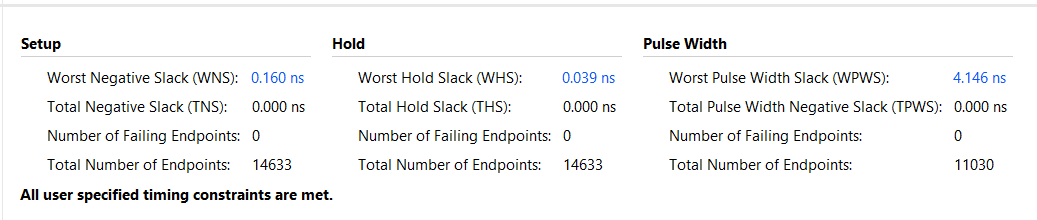
\includegraphics[width=0.8\textwidth]{Image/Timing.png}
    \label{fig:timing}
\end{figure}

Với chu kì xung nhịp 10ns trong tệp ràng buộc, báo cáo timing (Hình~\ref{fig:timing}) cho thấy thiết kế đạt tất cả ràng buộc
timing với WNS (Worst Negative Slack) = 0{,}160\,ns và WHS (Worst Hold Slack)
= 0{,}039\,ns, không có endpoint nào vi phạm. Điều này xác nhận thiết kế hoạt
động ổn định tại tần số 100\,MHz trên FPGA thực tế.

\begin{figure}[h]{Báo cáo công suất tiêu thụ ước tính}
    \centering
    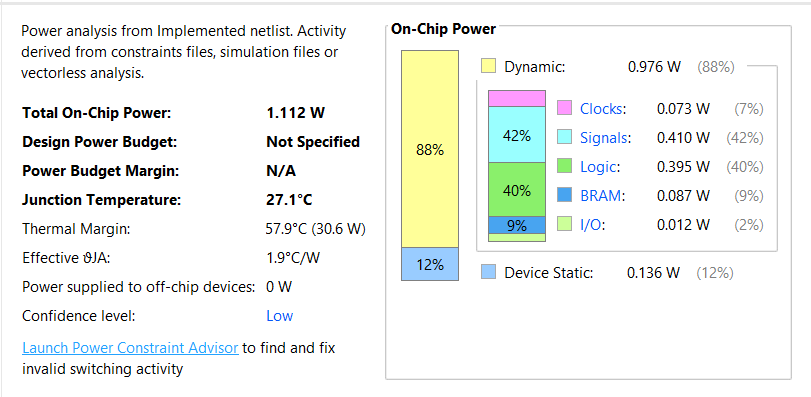
\includegraphics[width=0.6\textwidth]{Image/Power.png}
    \label{fig:power}
\end{figure}

Công suất tiêu thụ ước tính (Hình~\ref{fig:power}) là 1{,}112\,W tổng on-chip,
trong đó công suất động chiếm 0{,}976\,W (88\%) và công suất tĩnh 0{,}136\,W
(12\%). Phần lớn công suất động đến từ tín hiệu chuyển mạch (Signals: 0{,}410\,W)
và logic tổ hợp (Logic: 0{,}395\,W), phản ánh mật độ tính toán cao của các bộ nhân
và adder tree trong pipeline EMA. Nhiệt độ junction ước tính 27{,}1$^{\circ}$C,
nằm trong giới hạn an toàn của FPGA.

\section{Thiết lập và kiểm chứng trên phần cứng FPGA}
\subsection{Thiết lập thực nghiệm}

Sau khi tổng hợp chức năng thành công, thiết kế được tổng hợp và nạp xuống
FPGA Artix-7 XC7A200T trên bo mạch AC701 để kiểm chứng trên phần cứng thực tế.
Tương tự như trong mô phỏng, toàn bộ dữ liệu đầu vào (bản đồ đặc trưng, weight, bias,
tham số GroupNorm) được nạp sẵn trong BRAM ROM, bỏ qua bước ghi dữ liệu qua
cổng ngoài nhằm đơn giản hóa quá trình kiểm thử.

\begin{figure}[h]{Cấu trúc khối thiết kế trên FPGA: EMA + VIO + ILA}
    \centering
    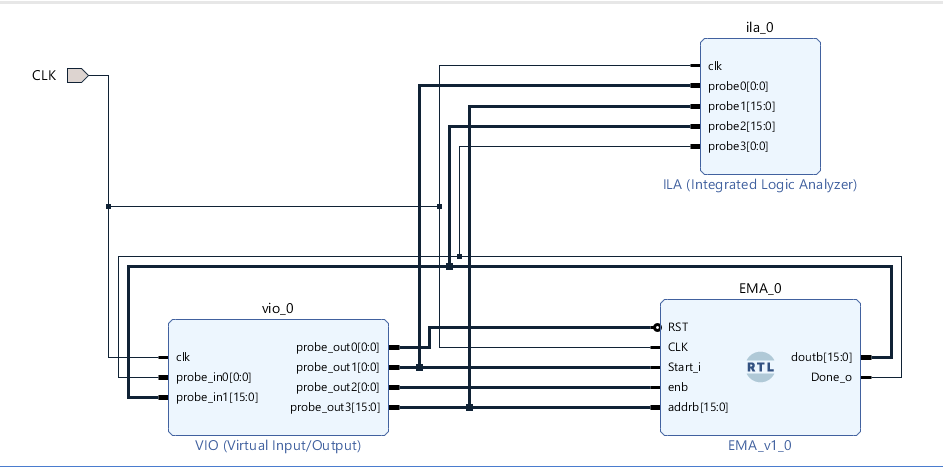
\includegraphics[width=0.9\textwidth]{Image/ILA_structure.png}
    \label{fig:ila_structure}
\end{figure}

Hình~\ref{fig:ila_structure} thể hiện cấu trúc khối kiểm thử gồm ba thành phần:
\begin{itemize}
    \item \textbf{EMA\_0:} Mô-đun EMA đã tổng hợp, với các cổng RST, CLK,
    Start\_i, enb, addrb[15:0] ở phía đầu vào và Done\_o, doutb[15:0] ở phía
    đầu ra.

    \item \textbf{VIO (Virtual Input/Output):} Cho phép điều khiển và quan sát
    tín hiệu từ máy tính qua cổng JTAG mà không cần thiết kế thêm logic giao
    tiếp. Bốn tín hiệu \texttt{probe\_out} điều khiển đầu vào của EMA:
    \texttt{probe\_out0} $\to$ RST, \texttt{probe\_out1} $\to$ Start\_i,
    \texttt{probe\_out2} $\to$ enb, \texttt{probe\_out3[15:0]} $\to$ addrb.
    Hai tín hiệu \texttt{probe\_in} đọc đầu ra: \texttt{probe\_in0} $\to$
    Done\_o, \texttt{probe\_in1[15:0]} $\to$ doutb.

    \item \textbf{ILA (Integrated Logic Analyzer):} Ghi lại dạng sóng các tín
    hiệu theo thời gian thực, bao gồm Done\_o, doutb, addrb và Start\_i. Dữ
    liệu được lưu trong BRAM nội bộ và hiển thị trên giao diện Vivado Hardware
    Manager.
\end{itemize}

Quy trình kiểm thử trên FPGA gồm bốn bước: (1)~Dùng VIO đặt RST~=~1 rồi
hạ về~0 để reset mô-đun; (2)~Đặt Start\_i~=~1 để khởi động tính toán;
(3)~Chờ Done\_o~=~1 báo hiệu hoàn tất; (4)~Bật enb~=~1 và lần lượt thay đổi
addrb từ 0 đến 4095 để đọc từng giá trị output qua doutb. ILA đồng thời ghi
lại toàn bộ dạng sóng trong quá trình chạy.

\section{Kiểm chứng trên phần cứng}

Sau khi nạp bitstream xuống bo mạch AC701, mô-đun EMA được kiểm thử theo quy trình
mô tả trong mục~5.1.

\begin{figure}[h]{Dạng sóng ILA1}
    \centering
    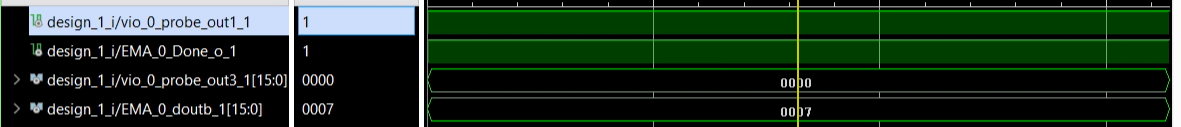
\includegraphics[width=\textwidth]{Image/ILA.png}
    \label{fig:ila1}
\end{figure}

\begin{figure}[h]{Dạng sóng ILA2}
    \centering
    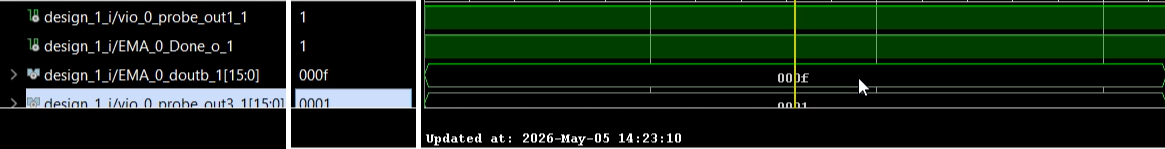
\includegraphics[width=\textwidth]{Image/ILA2.png}
    \label{fig:ila2}
\end{figure}

\begin{figure}[h]{Dạng sóng ILA3}
    \centering
    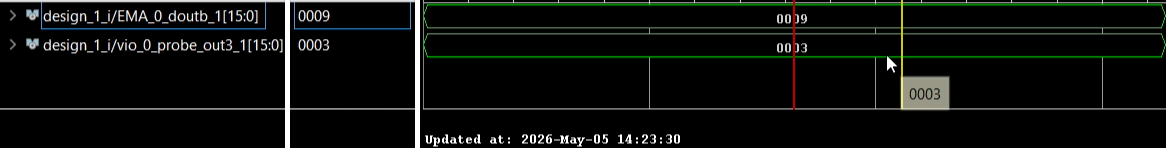
\includegraphics[width=\textwidth]{Image/ILA3.png}
    \label{fig:ila3}
\end{figure}

\newpage

Hình~\ref{fig:ila1}, \ref{fig:ila2} và \ref{fig:ila3} thể hiện dạng sóng ghi lại
bởi ILA tại ba vị trí output:
\begin{itemize}
    \item Hình~\ref{fig:ila1}: addrb = \texttt{0x0000}, doutb = \texttt{0x0007}
    --- khớp chính xác giá trị đầu tiên trong tệp tham chiếu Python.
    \item Hình~\ref{fig:ila2}: addrb = \texttt{0x0001}, doutb = \texttt{0x000F}
    --- tham chiếu Python là \texttt{0x000B}, sai lệch 4\,LSB, nằm trong phạm
    vi sai số đã phân tích ở mục~4.3.
    \item Hình~\ref{fig:ila3}: addrb = \texttt{0x0003}, doutb = \texttt{0x0009}
    --- tham chiếu Python là \texttt{0x0007}, sai lệch 2\,LSB.
\end{itemize}

Kết quả đầu ra trên FPGA thực tế nhất quán với kết quả mô phỏng hành vi trong
Vivado, xác nhận rằng thiết kế hoạt động đúng chức năng sau tổng hợp và
triển khai trên FPGA --- không xuất hiện sai lệch do tối ưu hóa logic hay timing.

\section{So sánh hiệu năng với phần mềm}

Để đánh giá hiệu năng thiết kế FPGA trong bối cảnh thực tế, mô-đun EMA được
benchmark trên nền tảng phần mềm PyTorch chạy trên CPU AMD Ryzen~7 6800H    . Mỗi benchmark chạy 4096 lần inference, lấy giá
trị trung bình. Đồ án sử dụng giá trị inf/s là số lượt suy luận trên mỗi giây---Chỉ số này đại diện cho số lượng khối dữ liệu đặc trưng mà kiến trúc phần cứng có thể xử lý hoàn chỉnh trong một giây(trong đồ án này là mảng đầu vào 4096 phần tử).

Do cửa sổ ghi của ILA có độ sâu hạn chế, không đủ bao phủ toàn bộ quá trình
xử lý từ khi Start tích cực đến khi Done tích cực, thời gian xử lý trên FPGA
được tính dựa trên tổng số chu kỳ đã xác định trong mô phỏng. Với 99.950 chu
kỳ cho một nhóm (16 kênh, không gian $16 \times 16$), tại tần số 100\,MHz
thời gian xử lý tương ứng khoảng 1{,}0\,ms.

\begin{table}[h]{So sánh thời gian xử lý 1 group EMA}
    \centering
    \begin{tabular}{|l|r|r|}
        \hline
        \textbf{Nền tảng} & \textbf{Thời gian} & \textbf{Throughput} \\
        \hline
        PyTorch CPU (4906 input)    & 340\,\textmu s  & 2{,}938 inf/s \\
        FPGA Artix-7 (1 group)         & 1{,}000\,\textmu s & 1{,}000 inf/s \\
        \hline
    \end{tabular}
    \label{tab:compare_1group}
\end{table}

Với 1 group ($C = 16$, $H = W = 16$), thiết kế FPGA chạy chậm hơn PyTorch CPU
khoảng 2{,}9 lần. Điều này là do PyTorch tận dụng thư viện MKL/OpenBLAS đã tối
ưu cao độ cho kiến trúc x86, trong khi thiết kế FPGA hiện tại xử lý Conv3$\times$3
chủ yếu tuần tự với chỉ 9 bộ nhân song song.

Tuy nhiên, mô-đun EMA trong ResNet50 hoạt động với $G = 32$ nhóm độc lập. Trên
FPGA, các group có thể được xử lý \textbf{song song hoàn toàn} bằng cách nhân bản
phần cứng, trong khi CPU phải xử lý tuần tự. Bảng~\ref{tab:compare_4group} so sánh
khi mở rộng sang 4 group song song:

\begin{table}[h]{So sánh khi mở rộng 4 group song song}
    \centering
    \begin{tabular}{|l|r|r|}
        \hline
        \textbf{Nền tảng} & \textbf{Thời gian} & \textbf{Throughput} \\
        \hline
        PyTorch CPU (16384 input)    & 1{,}780\,\textmu s  & 562 inf/s \\
        FPGA Artix-7 (4 group $\times$)& 1{,}000\,\textmu s  & 1{,}000 inf/s \\
        \hline
    \end{tabular}
    \label{tab:compare_4group}
\end{table}

Khi mở rộng sang 4 group song song, thời gian xử lý trên FPGA vẫn giữ nguyên
1{,}0\,ms (các group chạy đồng thời), trong khi PyTorch CPU tăng lên 1{,}78\,ms
do phải xử lý tuần tự qua 4 group với $C/G = 128$ kênh mỗi group. Ở cấu hình
này, FPGA đã \textbf{nhanh hơn CPU 1{,}78 lần}.

Ngoài tốc độ, FPGA còn có lợi thế lớn về công suất tiêu thụ: thiết kế 1 group
trên Artix-7 tiêu thụ khoảng 1\,W (theo ước tính từ Vivado), mở rộng 4 group
song song ước tính khoảng 3--4\,W. Trong khi đó CPU Ryzen~7 6800H có TDP 45\,W.
Với hiệu năng tương đương hoặc vượt trội, FPGA tiết kiệm năng lượng hơn hàng
chục lần so với CPU --- đây là ưu thế then chốt trong các ứng dụng inference AI
trên thiết bị biên, nơi ngân sách năng lượng bị giới hạn nghiêm ngặt.

\section{So sánh đối chứng với các công trình liên quan}
\label{sec:so_sanh}

Do số lượng các nghiên cứu hiện nay về việc tăng tốc phần cứng cơ chế chú ý chuyên biệt cho phân khúc thiết bị biên (Edge AI) còn tương đối hạn chế, phần này tiến hành chọn mẫu các kiến trúc tăng tốc tiên tiến nhất trên đa dạng phân khúc để làm rõ ràng ranh giới thiết kế, đồng thời định vị giá trị của lõi IP EMA được đề xuất.
Cụ thể, lõi IP EMA được đặt trong hệ quy chiếu so sánh với ba kiến trúc tiêu biểu:
\begin{itemize}
    \item \textbf{EfficientViT Accelerator (2024) \cite{efficientvit_acc}:} Kiến trúc tăng tốc mạng lai Convolution-Transformer sử dụng lượng tử hóa 8-bit trên mạch Edge cao cấp Zynq UltraScale+ ZCU102.
    \item \textbf{SWAT Accelerator (2024) \cite{swat_acc}:} Kiến trúc tăng tốc cơ chế chú ý cửa sổ sử dụng dấu phẩy động (FP16) trên card máy chủ dữ liệu khổng lồ Alveo U55C.
    \item \textbf{Sparse Attention (Peng và cộng sự, 2022) \cite{peng2022_sparse}:} Hệ thống tăng tốc chú ý bằng kỹ thuật xấp xỉ Top-K sử dụng dấu phẩy tĩnh 8-bit, triển khai trên card máy chủ Alveo U280.
\end{itemize}

\subsection{Tổng hợp các chỉ số hiệu năng và tài nguyên}

Bảng \ref{tab:so_sanh_tong_hop} trình bày chi tiết các thông số đo lường giữa lõi IP EMA và các công trình đối chứng.
% --- BẢNG SO SÁNH ĐÃ FIX TRÀN LỀ ---
\begin{table}[h]{So sánh tài nguyên, hiệu năng và công suất với các công trình liên quan}
\centering
\label{tab:so_sanh_tong_hop}
\renewcommand{\arraystretch}{1.3}
\footnotesize
\begin{tabular}{|p{2.6cm}|p{2.8cm}|p{3cm}|p{3cm}|p{3cm}|}
\hline
\textbf{Thông số / Tiêu chí} & \textbf{Đề xuất của đồ án} & \textbf{EfficientViT \cite{efficientvit_acc}} & \textbf{SWAT \cite{swat_acc}} & \textbf{Sparse Attn. \cite{peng2022_sparse}} \\ \hline
\textbf{Cơ chế tăng tốc} & EMA Attention & EfficientViT & Window Attn. & Sparse (Top-K) \\ \hline
\textbf{Nền tảng FPGA} & Artix-7 (XC7A200T) & UltraScale+ ZCU102 & Alveo U55C & Alveo U280 \\ \hline
\textbf{Định dạng dữ liệu} & Dấu phẩy tĩnh Q8.8 & Dấu phẩy tĩnh FIX8 & Dấu phẩy động FP16 & Dấu phẩy tĩnh 8-bit \\ \hline
\textbf{Tài nguyên LUT} & \textbf{42.767} & 104.463 & $\sim$494.000 & Chiếm phần lớn SLR0 \\ \hline
\textbf{Flip-Flop (FF)} & \textbf{10.875} & 249.473 & $\sim$286.000 & Rất lớn \\ \hline
\textbf{Khối nhân DSP} & \textbf{0} & 1.024 & Hàng ngàn khối & 3.000 \\ \hline
\textbf{Tần số xung nhịp} & \textbf{100 MHz} & 200 MHz & Tối ưu Pipeline & 200 MHz \\ \hline
\textbf{Công suất tiêu thụ} & \textbf{1,112 W} & 7,43 W & Hàng chục Watt & $\sim$35,3 W \\ \hline
\textbf{Phân khúc ứng dụng} & Edge AI & Edge AI & Trung tâm dữ liệu & Trung tâm dữ liệu \\ \hline
\end{tabular}
\end{table}

\subsection{Phân tích và thảo luận đánh giá}

Dựa trên dữ liệu từ Bảng \ref{tab:so_sanh_tong_hop}, các điểm ưu việt và sự đánh đổi (trade-off) trong thiết kế của đồ án được phân tích qua hai khía cạnh cốt lõi sau:

\textbf{Thứ nhất: Hiệu quả năng lượng và Tối ưu tài nguyên phần cứng (0 DSP).} 
Khi đặt cạnh các kiến trúc máy chủ dữ liệu lớn như SWAT \cite{swat_acc} hay hệ thống của Peng và cộng sự \cite{peng2022_sparse} – vốn phụ thuộc vào card Alveo đắt đỏ và tiêu thụ từ hàng chục đến hơn $35$ W điện – lõi IP EMA đề xuất chứng minh sự phù hợp tuyệt đối cho thiết bị biên với công suất siêu thấp chỉ $1,112$ W. 

Đặc biệt, khi so sánh cùng phân khúc thiết bị nhúng với công trình EfficientViT \cite{efficientvit_acc}, sự vượt trội về tài nguyên càng thể hiện rõ. Lõi IP của đồ án sử dụng định dạng \textbf{lượng tử hóa 16-bit (Q8.8)} – vốn đòi hỏi chi phí tính toán cao hơn – nhưng lại được thiết kế tối ưu tuyệt đối để sử dụng \textbf{0 DSP}. Trong khi đó, kiến trúc EfficientViT dù dùng chuẩn lượng tử hóa 8-bit thấp hơn vẫn tiêu tốn tới 1.024 khối DSP và $7,43$ W. Việc đồ án ánh xạ toàn bộ phép toán vào logic tổ hợp (LUT) mang lại tính linh hoạt (portability) tuyệt đối, cho phép triển khai mạch trên bất kỳ dòng FPGA phân khúc thấp nào mà không bị ràng buộc bởi phần cứng chuyên dụng (vendor lock-in).

\textbf{Thứ hai: Độ trễ thời gian thực và Năng lượng trên mỗi lượt suy luận.}
Công trình SWAT \cite{swat_acc} công bố khả năng xử lý chuỗi 4096 đầu vào trong khoảng $1$ ms trên phần cứng khổng lồ. Kết quả đo kiểm cho thấy lõi IP EMA của đồ án, dù chỉ hoạt động ở tần số 100 MHz, cũng hoàn thành xử lý khối 4096 phần tử đầu vào trong thời gian tương đương ($1$ ms). 

Quan trọng hơn, năng lượng tiêu hao cho mỗi lượt suy luận (Energy per Inference - $E_{inf}$) được xác định bằng tích của tổng công suất tiêu thụ on-chip ($P_{total} = 1,112$ W) với thời gian xử lý thực tế của một nhóm dữ liệu ($t_{inf} \approx 1,0$ ms):
\begin{equation}
    E_{inf} = P_{total} \times t_{inf} = 1,112 \text{ W} \times 1,0 \text{ ms} = 1,112 \text{ mJ}
\end{equation}
Nhờ vào việc duy trì mức công suất on-chip siêu thấp, chỉ số tiêu thụ năng lượng này của mạch thấp hơn hàng chục lần so với các hệ thống GPU hay FPGA máy chủ, tối ưu hóa triệt để cho bài toán triển khai Edge AI.

\subsection{Đánh giá khả năng mở rộng (Scalability)}

Mặc dù kiến trúc hiện tại (xử lý 1 cụm Channel/Group) đạt mức tối ưu tuyệt đối về năng lượng, việc mở rộng quy mô (ví dụ: nhân 4 lần luồng xử lý song song để tăng thông lượng) sẽ vấp phải rào cản vật lý. Việc nhân 4 lần tài nguyên logic tổ hợp sẽ đẩy lượng LUT ước tính lên mức $\sim$171.000 LUT, vượt quá giới hạn phần cứng của dòng chip Artix-7 XC7A200T (134.600 LUT). 

Tuy nhiên, điều này mở ra định hướng cho các nghiên cứu tiếp theo: (1) Nâng cấp lên các SoC FPGA có diện tích lớn hơn; hoặc (2) Cho phép công cụ tổng hợp tái kích hoạt và khai thác 740 khối DSP nhàn rỗi trên Artix-7 để giảm tải cho LUT. Dù ở kịch bản nào, công suất ước tính của phiên bản 4x vẫn chỉ nằm ở ngưỡng $\sim 4,5$ W, tiếp tục duy trì lợi thế lớn về tiết kiệm điện năng so với mức $7,43$ W của hệ thống EfficientViT (vốn chỉ chạy 8-bit) hiện hành.

\chapter{KẾT LUẬN}
\section{Tổng kết}

Đồ án đã hoàn thành mục tiêu đề ra: thiết kế, mô phỏng và tổng hợp thành công
lõi IP mức RTL cho mô-đun EMA (Efficient Multi-Scale Attention) bằng ngôn ngữ VHDL,
triển khai trên FPGA Artix-7 XC7A200T (bo mạch AC701). Đây là triển khai phần cứng
đầu tiên cho mô-đun chú ý EMA --- một cơ chế chú ý tiên tiến được công bố tại
ICASSP 2023, vốn chỉ tồn tại dưới dạng phần mềm PyTorch.

Thiết kế bao gồm 12 khối chức năng theo phương pháp FSMD (Finite State Machine with
Datapath) với biểu diễn số thực dấu phẩy tĩnh Q8.8 xuyên suốt: 3 bộ gộp
(AvgPoolH, AvgPoolW, AvgPool), 2 bộ tích chập (Conv1$\times$1, Conv3$\times$3 với
9 bộ nhân Booth-Wallace song song), 3 bộ chuẩn hóa và kích hoạt (GroupNorm, Sigmoid,
Softmax), 4 bộ tính toán chú ý (ElemMul, Matmul, AddSigmoid, FinalMul), cùng các
toán tử cơ bản hỗ trợ: bộ nhân Booth-Wallace, bộ chia Goldschmidt, bộ SQRT
Newton-Raphson và bộ Exponential pipeline. Toàn bộ được kết nối qua
mô-đun top-level EMA\_controller (FSM 14 trạng thái) và EMA\_datapath, giao tiếp qua
hệ thống BRAM nội bộ.

Các kết quả chính đạt được:

\begin{itemize}
    \item \textbf{Chức năng:} Mô-đun hoạt động đúng cả trong mô phỏng behavioral lẫn
    trên FPGA thực tế. So với mô hình Python tham chiếu (cùng bộ trọng số Q8.8 từ
    ResNet50+CIFAR-100, Top-1 = 80{,}69\%), sai số trung bình đạt 1{,}38\,LSB
    ($\approx 0{,}005$), với 96{,}85\% giá trị sai lệch $\leq 3$\,LSB. Kết quả
    trên FPGA (kiểm chứng qua ILA và VIO) nhất quán hoàn toàn với thử nghiệm, xác nhận
    thiết kế không bị ảnh hưởng bởi tối ưu hóa logic hay timing.

    \item \textbf{Hiệu năng:} Tổng thời gian xử lý 1 group (16 kênh, $16 \times 16$)
    là 99{,}950 chu kỳ, tương ứng $\sim$1{,}0\,ms tại 100\,MHz. FSM top-level khai
    thác song song: Conv3$\times$3 chạy đồng thời với toàn bộ nhánh~1, hai instance
    AvgPool/Softmax/Matmul chạy song song. Khi mở rộng 4 group song song, FPGA đạt
    1{,}0\,ms --- nhanh hơn 1{,}78 lần so với PyTorch CPU trên AMD Ryzen~7 6800H
    (1{,}78\,ms).

    \item \textbf{Tài nguyên:} 42{,}767 LUT (31{,}96\%), 10{,}875 FF (4{,}06\%),
    43{,}5 BRAM (11{,}92\%) trên XC7A200T --- còn dư đáng kể cho mở rộng.

    \item \textbf{Timing:} Đạt tất cả ràng buộc timing. Với tần số ràng buộc 100\,MHz (chu kỳ 10\,ns) và WNS = 0{,}160\,ns, tần số hoạt động tối đa $f_{max} = 1/(10 - 0{,}160) \approx 101{,}6$\,MHz.

    \item \textbf{Công suất:} Tổng on-chip power ước tính 1{,}112\,W cho 1 group,
    ước tính 3--4\,W cho 4 group song song --- tiết kiệm hơn hàng chục lần so với
    CPU (TDP 45\,W) ở cùng mức throughput.
\end{itemize}

\section{Hạn chế}

\begin{itemize}
    \item Thiết kế hiện tại chỉ triển khai 1 trong 32 group của mô-đun EMA. Việc mở
    rộng ra toàn bộ 32 group song song đòi hỏi tài nguyên FPGA lớn hơn hoặc cơ chế
    chia sẻ thời gian.

    \item Conv3$\times$3 chiếm 86{,}017 trong tổng 99{,}950 chu kỳ (86\%), là nút
    thắt cổ chai rõ ràng. Nguyên nhân do vòng lặp IC ($C = 16$) xử lý tuần tự với
    chỉ 9 bộ nhân song song theo 9 vị trí kernel.

    \item Các khối chức năng hoạt động chủ yếu tuần tự (trừ song song giữa
    Conv3$\times$3 và nhánh~1), chưa có pipelining giữa các khối nên mỗi khối phải
    chờ khối trước hoàn tất hoàn toàn.
\end{itemize}

\section{Hướng phát triển}

\begin{itemize}
    \item \textbf{Tối ưu Conv3$\times$3:} Tăng số bộ nhân song song theo chiều IC
    (ví dụ: xử lý 2 hoặc 4 kênh IC đồng thời) hoặc áp dụng line buffer để tái sử
    dụng dữ liệu đầu vào, giảm số lần đọc BRAM và giảm bottleneck 86{,}017 chu kỳ
    hiện tại.

    \item \textbf{Pipelining giữa các khối:} Cho phép khối sau bắt đầu xử lý ngay
    khi khối trước xuất ra kết quả từng phần (ví dụ: GroupNorm bắt đầu khi ElemMul
    hoàn thành từng kênh), chuyển từ mô hình ``chờ hoàn tất'' sang mô hình
    ``streaming'', tăng throughput tổng thể.

    \item \textbf{Mở rộng đa group:} Nhân bản phần cứng 4--8 group song song trên
    XC7A200T (tài nguyên cho phép), hoặc thiết kế cơ chế chia sẻ thời gian (1 bộ
    phần cứng xử lý luân phiên 32 group) để cân bằng giữa tài nguyên và throughput.

\end{itemize}

\begin{thebibliography}{99}
\begin{bibsection}{Tiếng Anh}
\bibitem{swat_acc}
Z. Bai, P. Dangi, H. Li, and T. Mitra, ``SWAT: Scalable and Efficient Window Attention-based Transformers Acceleration on FPGAs,'' in \textit{Proceedings of the 61st ACM/IEEE Design Automation Conference (DAC)}, 2024, pp. 1--6.

\bibitem{fixedpoint_exp}
M. Chandra, ``On the Implementation of Fixed-point Exponential Function for Machine Learning and Signal Processing Accelerators,'' \textit{IEEE Design \& Test}, vol. 39, no. 2, 2022, pp. 44--51.

\bibitem{goldschmidt1964}
R. E. Goldschmidt, ``Applications of Division by Convergence,'' M.S. thesis, Massachusetts Institute of Technology, Cambridge, MA, USA, 1964.

\bibitem{resnet2016}
K. He, X. Zhang, S. Ren, and J. Sun, ``Deep Residual Learning for Image Recognition,'' in \textit{Proceedings of the IEEE Conference on Computer Vision and Pattern Recognition (CVPR)}, 2016, pp. 770--778.

\bibitem{ca2021}
Q. Hou, D. Zhou, and J. Feng, ``Coordinate Attention for Efficient Mobile Network Design,'' in \textit{Proceedings of the IEEE/CVF Conference on Computer Vision and Pattern Recognition (CVPR)}, 2021, pp. 13713--13722.

\bibitem{se2018}
J. Hu, L. Shen, and G. Sun, ``Squeeze-and-Excitation Networks,'' in \textit{Proceedings of the IEEE/CVF Conference on Computer Vision and Pattern Recognition (CVPR)}, 2018, pp. 7132--7141.

\bibitem{korzilius2023}
S. Korzilius and B. Schoenmakers, ``Divisions and Square Roots with Tight Error Analysis from Newton–Raphson Iteration in Secure Fixed-Point Arithmetic,'' \textit{Cryptography}, vol. 7, no. 4, 2023, p. 43.

\bibitem{cifar2009}
A. Krizhevsky, ``Learning Multiple Layers of Features from Tiny Images,'' University of Toronto, Toronto, ON, Canada, Tech. Rep., 2009.

\bibitem{booth_wallace}
A. S. N. Mokhtar, N. Zahari, C. S. Ping, N. Ismail, and A. S. Ismail, ``Implementation of Modified Booth-Wallace Tree Multiplier in FPGA,'' \textit{Zulfaqar Journal of Defence Science, Engineering \& Technology}, vol. 5, no. 2, 2022, pp. 59--69.

\bibitem{cnn_intro2015}
K. O'Shea and R. Nash, ``An Introduction to Convolutional Neural Networks,'' \textit{arXiv preprint arXiv:1511.08458}, 2015.

\bibitem{ema2023}
D. Ouyang, S. He, G. Zhang, M. Luo, H. Guo, J. Zhan, and Z. Huang, ``Efficient Multi-Scale Attention Module with Cross-Spatial Learning,'' in \textit{Proceedings of the IEEE International Conference on Acoustics, Speech and Signal Processing (ICASSP)}, 2023, pp. 1--5.

\bibitem{peng2022_sparse}
H. Peng, Shaoyi Huang, Shiyang Chen, B. Li, T. Geng, and Caiwen Ding, ``A Length Adaptive Algorithm-Hardware Co-design of Transformer on FPGA Through Sparse Attention and Dynamic Pipelining,'' in \textit{Proceedings of the 59th ACM/IEEE Design Automation Conference (DAC)}, 2022, pp. 1--6.

\bibitem{efficientvit_acc}
H. Shao, H. Shi, W. Mao, and Z. Wang, ``An FPGA-Based Reconfigurable Accelerator for Convolution-Transformer Hybrid EfficientViT,'' in \textit{Proceedings of the IEEE International Symposium on Circuits and Systems (ISCAS)}, 2024, pp. 1--5.

\bibitem{eca2020}
Q. Wang, B. Wu, P. Zhu, P. Li, W. Zuo, and Q. Hu, ``ECA-Net: Efficient Channel Attention for Deep Convolutional Neural Networks,'' in \textit{Proceedings of the IEEE/CVF Conference on Computer Vision and Pattern Recognition (CVPR)}, 2020, pp. 11534--11542.

\bibitem{cbam2018}
S. Woo, J. Park, J.-Y. Lee, and I. S. Kweon, ``CBAM: Convolutional Block Attention Module,'' in \textit{Proceedings of the European Conference on Computer Vision (ECCV)}, 2018, pp. 3--19.
\end{bibsection}
\end{thebibliography}
\end{document}
